% Options for packages loaded elsewhere
% Options for packages loaded elsewhere
\PassOptionsToPackage{unicode}{hyperref}
\PassOptionsToPackage{hyphens}{url}
\PassOptionsToPackage{dvipsnames,svgnames,x11names}{xcolor}
%
\documentclass[
  letterpaper,
  DIV=11,
  numbers=noendperiod]{scrreprt}
\usepackage{xcolor}
\usepackage[top=25mm,left=20mm,right=20mm]{geometry}
\usepackage{amsmath,amssymb}
\setcounter{secnumdepth}{5}
\usepackage{iftex}
\ifPDFTeX
  \usepackage[T1]{fontenc}
  \usepackage[utf8]{inputenc}
  \usepackage{textcomp} % provide euro and other symbols
\else % if luatex or xetex
  \usepackage{unicode-math} % this also loads fontspec
  \defaultfontfeatures{Scale=MatchLowercase}
  \defaultfontfeatures[\rmfamily]{Ligatures=TeX,Scale=1}
\fi
\usepackage{lmodern}
\ifPDFTeX\else
  % xetex/luatex font selection
  \setmainfont[]{Times New Roman}
\fi
% Use upquote if available, for straight quotes in verbatim environments
\IfFileExists{upquote.sty}{\usepackage{upquote}}{}
\IfFileExists{microtype.sty}{% use microtype if available
  \usepackage[]{microtype}
  \UseMicrotypeSet[protrusion]{basicmath} % disable protrusion for tt fonts
}{}
\makeatletter
\@ifundefined{KOMAClassName}{% if non-KOMA class
  \IfFileExists{parskip.sty}{%
    \usepackage{parskip}
  }{% else
    \setlength{\parindent}{0pt}
    \setlength{\parskip}{6pt plus 2pt minus 1pt}}
}{% if KOMA class
  \KOMAoptions{parskip=half}}
\makeatother
% Make \paragraph and \subparagraph free-standing
\makeatletter
\ifx\paragraph\undefined\else
  \let\oldparagraph\paragraph
  \renewcommand{\paragraph}{
    \@ifstar
      \xxxParagraphStar
      \xxxParagraphNoStar
  }
  \newcommand{\xxxParagraphStar}[1]{\oldparagraph*{#1}\mbox{}}
  \newcommand{\xxxParagraphNoStar}[1]{\oldparagraph{#1}\mbox{}}
\fi
\ifx\subparagraph\undefined\else
  \let\oldsubparagraph\subparagraph
  \renewcommand{\subparagraph}{
    \@ifstar
      \xxxSubParagraphStar
      \xxxSubParagraphNoStar
  }
  \newcommand{\xxxSubParagraphStar}[1]{\oldsubparagraph*{#1}\mbox{}}
  \newcommand{\xxxSubParagraphNoStar}[1]{\oldsubparagraph{#1}\mbox{}}
\fi
\makeatother


\usepackage{longtable,booktabs,array}
\usepackage{calc} % for calculating minipage widths
% Correct order of tables after \paragraph or \subparagraph
\usepackage{etoolbox}
\makeatletter
\patchcmd\longtable{\par}{\if@noskipsec\mbox{}\fi\par}{}{}
\makeatother
% Allow footnotes in longtable head/foot
\IfFileExists{footnotehyper.sty}{\usepackage{footnotehyper}}{\usepackage{footnote}}
\makesavenoteenv{longtable}
\usepackage{graphicx}
\makeatletter
\newsavebox\pandoc@box
\newcommand*\pandocbounded[1]{% scales image to fit in text height/width
  \sbox\pandoc@box{#1}%
  \Gscale@div\@tempa{\textheight}{\dimexpr\ht\pandoc@box+\dp\pandoc@box\relax}%
  \Gscale@div\@tempb{\linewidth}{\wd\pandoc@box}%
  \ifdim\@tempb\p@<\@tempa\p@\let\@tempa\@tempb\fi% select the smaller of both
  \ifdim\@tempa\p@<\p@\scalebox{\@tempa}{\usebox\pandoc@box}%
  \else\usebox{\pandoc@box}%
  \fi%
}
% Set default figure placement to htbp
\def\fps@figure{htbp}
\makeatother





\setlength{\emergencystretch}{3em} % prevent overfull lines

\providecommand{\tightlist}{%
  \setlength{\itemsep}{0pt}\setlength{\parskip}{0pt}}



 



% --- Fix Horizontal Rules (---) ---
% Save the original \rule command so we can still use it later
\let\oldrule\rule

% Redefine \rule to check if it's the specific one generated by Pandoc for '---'
\renewcommand{\rule}[2]{%
  % Check: Is the requested width exactly 50% of the line width?
  % (Pandoc converts markdown '---' to \rule{0.5\linewidth} by default)
  \ifdim#1=0.5\linewidth
    \hrule % If yes, replace it with a full-width horizontal rule
  \else
    \oldrule{#1}{#2} % If no, draw the rule exactly as requested originally
  \fi
}

% --- Force Equation Numbering ---
% Redefine standard display math \[ ... \] to use the numbered 'equation' environment
% This ensures $$...$$ in Markdown gets numbered in the PDF
\renewcommand{\[}{\begin{equation}}
\renewcommand{\]}{\end{equation}}

\usepackage[most]{tcolorbox}

% --- Color Definitions ---
% Theorem group (Theorem, Lemma, Corollary, Proposition)
\definecolor{thm-bg}{HTML}{F0F7FF}
\definecolor{thm-frame}{HTML}{CFE2FF}

% Definition
\definecolor{def-bg}{HTML}{F0FFF4}
\definecolor{def-frame}{HTML}{BADBCC}

% Example
\definecolor{ex-bg}{HTML}{FFFBF0}
\definecolor{ex-frame}{HTML}{FFEEBB}

% Proof
\definecolor{proof-bg}{HTML}{E2E3E5}
\definecolor{proof-frame}{HTML}{E2E3E5}

% Solution
\definecolor{sol-bg}{HTML}{F9F2F4}
\definecolor{sol-frame}{HTML}{D9534F}

% --- Box Environments ---

% Theorem
\tcolorboxenvironment{theorem}{
  colback=thm-bg,
  colframe=thm-frame,
  boxrule=0pt,
  sharp corners,
  left=5pt, right=5pt,
  top=5pt, bottom=5pt,
  breakable
}

\tcolorboxenvironment{algorithm}{
  colback=thm-bg,
  colframe=thm-frame,
  boxrule=0pt,
  sharp corners,
  left=5pt, right=5pt,
  top=5pt, bottom=5pt,
  breakable
}


% Lemma
\tcolorboxenvironment{lemma}{
  colback=thm-bg,
  colframe=thm-frame,
  boxrule=0pt,
  sharp corners,
  left=5pt, right=5pt,
  top=5pt, bottom=5pt,
  breakable
}

% Corollary
\tcolorboxenvironment{corollary}{
  colback=thm-bg,
  colframe=thm-frame,
  boxrule=0pt,
  sharp corners,
  left=5pt, right=5pt,
  top=5pt, bottom=5pt,
  breakable
}

% Proposition
\tcolorboxenvironment{proposition}{
  colback=thm-bg,
  colframe=thm-frame,
  boxrule=0pt,
  sharp corners,
  left=5pt, right=5pt,
  top=5pt, bottom=5pt,
  breakable
}

% Definition
\tcolorboxenvironment{definition}{
  colback=def-bg,
  colframe=def-frame,
  boxrule=0pt,
  sharp corners,
  left=5pt, right=5pt,
  top=5pt, bottom=5pt,
  breakable
}

% Example
\tcolorboxenvironment{example}{
  colback=ex-bg,
  colframe=ex-frame,
  boxrule=0pt,
  sharp corners,
  left=5pt, right=5pt,
  top=5pt, bottom=5pt,
  breakable
}

% Proof
\tcolorboxenvironment{proof}{
  colback=proof-bg,
  colframe=proof-frame,
  boxrule=0pt,
  sharp corners,
  left=5pt, right=5pt,
  top=5pt, bottom=5pt,
  breakable
}

% Solution
\tcolorboxenvironment{sol}{
  colback=sol-bg,
  colframe=sol-frame,
  boxrule=0pt,
  sharp corners,
  left=5pt, right=5pt,
  top=5pt, bottom=5pt,
  breakable
}
\KOMAoption{captions}{tableheading}
\makeatletter
\@ifpackageloaded{tcolorbox}{}{\usepackage[skins,breakable]{tcolorbox}}
\@ifpackageloaded{fontawesome5}{}{\usepackage{fontawesome5}}
\definecolor{quarto-callout-color}{HTML}{909090}
\definecolor{quarto-callout-note-color}{HTML}{0758E5}
\definecolor{quarto-callout-important-color}{HTML}{CC1914}
\definecolor{quarto-callout-warning-color}{HTML}{EB9113}
\definecolor{quarto-callout-tip-color}{HTML}{00A047}
\definecolor{quarto-callout-caution-color}{HTML}{FC5300}
\definecolor{quarto-callout-color-frame}{HTML}{acacac}
\definecolor{quarto-callout-note-color-frame}{HTML}{4582ec}
\definecolor{quarto-callout-important-color-frame}{HTML}{d9534f}
\definecolor{quarto-callout-warning-color-frame}{HTML}{f0ad4e}
\definecolor{quarto-callout-tip-color-frame}{HTML}{02b875}
\definecolor{quarto-callout-caution-color-frame}{HTML}{fd7e14}
\makeatother
\makeatletter
\@ifpackageloaded{bookmark}{}{\usepackage{bookmark}}
\makeatother
\makeatletter
\@ifpackageloaded{caption}{}{\usepackage{caption}}
\AtBeginDocument{%
\ifdefined\contentsname
  \renewcommand*\contentsname{Table of contents}
\else
  \newcommand\contentsname{Table of contents}
\fi
\ifdefined\listfigurename
  \renewcommand*\listfigurename{List of Figures}
\else
  \newcommand\listfigurename{List of Figures}
\fi
\ifdefined\listtablename
  \renewcommand*\listtablename{List of Tables}
\else
  \newcommand\listtablename{List of Tables}
\fi
\ifdefined\figurename
  \renewcommand*\figurename{Figure}
\else
  \newcommand\figurename{Figure}
\fi
\ifdefined\tablename
  \renewcommand*\tablename{Table}
\else
  \newcommand\tablename{Table}
\fi
}
\@ifpackageloaded{float}{}{\usepackage{float}}
\floatstyle{ruled}
\@ifundefined{c@chapter}{\newfloat{codelisting}{h}{lop}}{\newfloat{codelisting}{h}{lop}[chapter]}
\floatname{codelisting}{Listing}
\newcommand*\listoflistings{\listof{codelisting}{List of Listings}}
\usepackage{amsthm}
\theoremstyle{definition}
\newtheorem{example}{Example}[chapter]
\theoremstyle{plain}
\newtheorem{theorem}{Theorem}[chapter]
\theoremstyle{plain}
\newtheorem{algorithm}{Algorithm}[chapter]
\theoremstyle{plain}
\newtheorem{lemma}{Lemma}[chapter]
\theoremstyle{definition}
\newtheorem{definition}{Definition}[chapter]
\theoremstyle{plain}
\newtheorem{corollary}{Corollary}[chapter]
\theoremstyle{remark}
\AtBeginDocument{\renewcommand*{\proofname}{Proof}}
\newtheorem*{remark}{Remark}
\newtheorem*{solution}{Solution}
\newtheorem{refremark}{Remark}[chapter]
\newtheorem{refsolution}{Solution}[chapter]
\makeatother
\makeatletter
\makeatother
\makeatletter
\@ifpackageloaded{caption}{}{\usepackage{caption}}
\@ifpackageloaded{subcaption}{}{\usepackage{subcaption}}
\makeatother
\usepackage{bookmark}
\IfFileExists{xurl.sty}{\usepackage{xurl}}{} % add URL line breaks if available
\urlstyle{same}
\hypersetup{
  pdftitle={Theory of Linear Models},
  pdfauthor={Longhai Li},
  colorlinks=true,
  linkcolor={blue},
  filecolor={Maroon},
  citecolor={Blue},
  urlcolor={Blue},
  pdfcreator={LaTeX via pandoc}}


\title{Theory of Linear Models}
\author{Longhai Li}
\date{2026-01-25}
\begin{document}
\maketitle


\bookmarksetup{startatroot}

\chapter*{Preface}\label{preface}
\addcontentsline{toc}{chapter}{Preface}

\markboth{Preface}{Preface}

\section*{Key Features}\label{key-features}
\addcontentsline{toc}{section}{Key Features}

\markright{Key Features}

This text adopts a geometric approach to the statistical theory of
linear models, aiming to provide a deeper understanding than standard
algebraic treatments. Key features include:

\begin{itemize}
\item
  \textbf{Projection Perspective:} We prioritize the geometric
  interpretation of least squares, viewing estimation as a projection of
  the response vector onto a model subspace. This visual framework
  unifies diverse topics---from simple regression to complex ANOVA
  designs---under a single theoretical umbrella.
\item
  \textbf{Interactive Visualizations:} Abstract concepts are brought to
  life through interactive 3D plots. Readers can rotate and inspect
  vector spaces, residual planes, and projection geometries to build a
  tangible intuition for high-dimensional operations.
\item
  \textbf{Computational Integration:} Theory is seamlessly integrated
  with practice. The text provides implementation examples using R (and
  Python), demonstrating how theoretical matrix equations translate
  directly into computational code.
\item
  \textbf{Rigorous Foundations:} While visually driven, the text
  maintains mathematical rigor, covering essential topics such as
  spectral theory, the generalized inverseand the multivariate normal
  distribution to ensure a solid theoretical grounding.
\end{itemize}

\section*{\texorpdfstring{\textbf{Overview}}{Overview}}\label{overview}
\addcontentsline{toc}{section}{\textbf{Overview}}

\markright{\textbf{Overview}}

This course is a rigorous examination of the general linear models using
vector space theory, in particular the approach of regarding least
square as projection. The topics includes: vector space; projection;
matrix algebra; generalized inverses; quadratic forms; theory for point
estimation; theory for hypothesis test; theory for non-full-rank models.

\section*{\texorpdfstring{\textbf{Audience}}{Audience}}\label{audience}
\addcontentsline{toc}{section}{\textbf{Audience}}

\markright{\textbf{Audience}}

This book is designed for graduate students and advanced undergraduate
students in statistics, data science, and related quantitative fields.
It serves as a bridge between applied regression analysis and the
theoretical foundations of linear models. Researchers and practitioners
seeking a deeper geometric and algebraic understanding of the
statistical methods they use daily will also find this text valuable.

\section*{\texorpdfstring{\textbf{Prerequisites}}{Prerequisites}}\label{prerequisites}
\addcontentsline{toc}{section}{\textbf{Prerequisites}}

\markright{\textbf{Prerequisites}}

To get the most out of this book, readers should have a comfortable
grasp of the following topics:

\textbf{Linear Algebra}: An elementary understanding of matrix
operations is essential. You should be familiar with matrix
multiplication, determinants, inversion, and the basic concepts of
vector spaces (such as linear independence, basis vectors, and
subspaces). While we review key spectral theory concepts (like
eigenvalues and the singular value decomposition) in the early chapters,
prior exposure to these ideas is helpful.

\textbf{Probability and Statistics}: A standard introductory course in
probability and mathematical statistics is required. Readers should be
familiar with random variables, expectation, variance, covariance,
common probability distributions (especially the Normal distribution),
and fundamental concepts of hypothesis testing and estimation.

\bookmarksetup{startatroot}

\chapter{Introduction}\label{introduction}

\section{Multiple Linear Regression}\label{multiple-linear-regression}

Suppose we have observations on \(Y\) and \(X_j\). The data can be
represented in matrix form.

\[
\underset{n \times 1}{y} = \underset{n \times p}{X} \beta + \underset{n \times 1}{\epsilon}
\]

where the error terms are distributed as: \[
\epsilon \sim N_n(0, \sigma^2 I_n),
\]

in which \(I_n\) is the identity matrix: \[
I_n = \begin{pmatrix} 
1 & 0 & \dots & 0 \\ 
0 & 1 & \dots & 0 \\ 
\vdots & \vdots & \ddots & \vdots \\ 
0 & 0 & \dots & 1 
\end{pmatrix}
\] The scalar equation for a single observation is: \[
Y_i = \beta_0 + \beta_1 X_{i1} + \dots + \beta_p X_{ip} + \epsilon_i
\]

\section{Examples}\label{examples}

\subsection{Polynomial Regression}\label{polynomial-regression}

Polynomial regression fits a curved line to the data points but remains
linear in the parameters (\(\beta\)).

The model equation is: \[
y_i = \beta_0 + \beta_1 x_i + \beta_2 x_i^2 + \dots + \beta_{p-1} x_i^{p-1}
\]

\subsection{Design Matrix
Construction}\label{design-matrix-construction}

The design matrix \(X\) is constructed by taking powers of the input
variable.

\[
y = \begin{pmatrix} y_1 \\ \vdots \\ y_n \end{pmatrix} = 
\begin{pmatrix} 
1 & x_1 & x_1^2 & \dots & x_1^{p-1} \\ 
1 & x_2 & x_2^2 & \dots & x_2^{p-1} \\ 
\vdots & \vdots & \vdots & \ddots & \vdots \\ 
1 & x_n & x_n^2 & \dots & x_n^{p-1} 
\end{pmatrix} 
\begin{pmatrix} \beta_0 \\ \beta_1 \\ \vdots \\ \beta_{p-1} \end{pmatrix} + 
\begin{pmatrix} \epsilon_1 \\ \epsilon_2 \\ \vdots \\ \epsilon_n \end{pmatrix}
\]

\subsection{One-Way ANOVA}\label{one-way-anova}

ANOVA can be expressed as a linear model using categorical predictors
(dummy variables).

Suppose we have 3 groups (\(G_1, G_2, G_3\)) with observations: \[
Y_{ij} = \mu_i + \epsilon_{ij}, \quad \epsilon_{ij} \sim N(0, \sigma^2)
\]

\[
\overset{G_1}{
  \boxed{
    \begin{matrix} Y_{11} \\ Y_{12} \end{matrix}
  }
}
\quad
\overset{G_2}{
  \boxed{
    \begin{matrix} Y_{21} \\ Y_{22} \end{matrix}
  }
}
\quad
\overset{G_3}{
  \boxed{
    \begin{matrix} Y_{31} \\ Y_{32} \end{matrix}
  }
}
\]

We construct the matrix \(X\) to select the group mean (\(\mu\))
corresponding to the observation:

\[
\underset{6 \times 1}{y} = \underset{6 \times 3}{X} \begin{pmatrix} \mu_1 \\ \mu_2 \\ \mu_3 \end{pmatrix} + \epsilon
\]

\[
\begin{bmatrix}
Y_{11} \\ Y_{12} \\ Y_{21} \\ Y_{22} \\ Y_{31} \\ Y_{32}
\end{bmatrix} = 
\begin{bmatrix}
1 & 0 & 0 \\
1 & 0 & 0 \\
0 & 1 & 0 \\
0 & 1 & 0 \\
0 & 0 & 1 \\
0 & 0 & 1
\end{bmatrix}
\begin{bmatrix}
\mu_1 \\ \mu_2 \\ \mu_3
\end{bmatrix} + \epsilon
\]

\subsection{Analysis of Covariance
(ANCOVA)}\label{analysis-of-covariance-ancova}

ANCOVA combines continuous variables and categorical (dummy) variables
in the same design matrix.

\[
\begin{bmatrix}
Y_1 \\ \vdots \\ Y_n
\end{bmatrix} =
\begin{bmatrix}
X_{1,\text{cont}} & 1 & 0 \\
X_{2,\text{cont}} & 1 & 0 \\
\vdots & 0 & 1 \\
X_{n,\text{cont}} & 0 & 1
\end{bmatrix} \beta + \epsilon
\]

\section{Least Squares Estimation}\label{least-squares-estimation}

For the general linear model \(y = X\beta + \epsilon\), the Least
Squares estimator is:

\[
\hat{\beta} = (X'X)^{-1}X'y
\]

The predicted values (\(\hat{y}\)) are obtained via the Projection
Matrix (Hat Matrix) \(P_X\):

\[
\hat{y} = X\hat{\beta} = X(X'X)^{-1}X'y = P_X y
\]

The residuals and Sum of Squared Errors are:

\[
\hat{e} = y - \hat{y}
\] \[
\text{SSE} = ||\hat{e}||^2
\]

The coefficient of determination is: \[
R^2 = \frac{\text{SST} - \text{SSE}}{\text{SST}}
\] where \(\text{SST} = \sum (y_i - \bar{y})^2\).

\section{Geometric Perspective of Least Square
Estimation}\label{geometric-perspective-of-least-square-estimation}

We align the coordinate system to the models for clarity:

\begin{enumerate}
\def\labelenumi{\arabic{enumi}.}
\tightlist
\item
  \textbf{Reduced Model (}\(M_0\)): Represented by the \textbf{X-axis}
  (labeled \(j_3\)).

  \begin{itemize}
  \tightlist
  \item
    \(\hat{y}_0\) is the projection of \(y\) onto this axis.
  \end{itemize}
\item
  \textbf{Full Model (}\(M_1\)): Represented by the \textbf{XY-plane}
  (the floor).

  \begin{itemize}
  \tightlist
  \item
    \(\hat{y}_1\) is the projection of \(y\) onto this plane (\(z=0\)).
  \end{itemize}
\item
  \textbf{Observed Data (}\(y\)): A point in 3D space.
\end{enumerate}

The ``improvement'' due to adding predictors is the distance between
\(\hat{y}_0\) and \(\hat{y}_1\).

\begin{figure}

\centering{

\includegraphics[width=0.9\linewidth,height=\textheight,keepaspectratio]{figs/3d-lm.png}

}

\caption{\label{fig-geometry-simple}Geometric Interpretation: Projection
onto Axis (M0) vs Plane (M1)}

\end{figure}%

The geometric perspective is not merely for intuition, but as the most
robust framework for mastering linear models. This approach offers three
distinct advantages:

\begin{itemize}
\tightlist
\item
  \textbf{Statistical Clarity:} Geometry provides the most natural path
  to understanding the properties of estimators. By viewing least square
  estimation as an orthogonal projection, the decomposition of sums of
  squares into independent components becomes visually obvious,
  demystifying how degrees of freedom relate to subspace dimensions
  rather than abstract algebraic constants. The sampling distribution of
  the sum squares become straightforward.
\item
  \textbf{Computational Stability:} A geometric understanding is
  essential for implementing efficient and numerically stable
  algorithms. While the algebraic ``Normal Equations''
  (\((X'X)^{-1}X'y\)) are theoretically valid, they are often
  computationally hazardous. The geometric approach leads directly to
  superior methods---such as QR and Singular Value Decompositions---that
  are the backbone of modern statistical software.
\item
  \textbf{Generalizability:} The principles of projection and
  orthogonality extend far beyond the Gaussian linear model. These
  geometric insights provide the foundational intuition needed for
  tackling non-Gaussian optimization problems, including Generalized
  Linear Models (GLMs) and convex optimization, where solutions can
  often be viewed as projections onto convex sets.
\end{itemize}

\bookmarksetup{startatroot}

\chapter{Projection in Vector Space}\label{projection-in-vector-space}

\section{Vector and Projection onto a
Line}\label{vector-and-projection-onto-a-line}

\subsection{Vectors and Operations}\label{vectors-and-operations}

The concept of a vector is fundamental to linear algebra and linear
models. We begin by formally defining what a vector is in the context of
Euclidean space.

\begin{definition}[Vector]\protect\hypertarget{def-vector}{}\label{def-vector}

A \textbf{vector} \(x\) is defined as a point in \(n\)-dimensional space
(\(\mathbb{R}^n\)). It is typically represented as a column vector
containing \(n\) real-valued components: \[
x = \begin{pmatrix} x_1 \\ x_2 \\ \vdots \\ x_n \end{pmatrix}
\]

\end{definition}

Vectors are not just static points; they can be combined and
manipulated. The two most basic geometric operations are addition and
subtraction.

\textbf{Vector Arithmetic:} Vectors can be manipulated geometrically:

\begin{definition}[Vector
Addition]\protect\hypertarget{def-vector-addition}{}\label{def-vector-addition}

The sum of two vectors \(x\) and \(y\) creates a new vector. The
operation is performed component-wise, adding corresponding elements
from each vector. Geometrically, this follows the ``parallelogram rule''
or the ``head-to-tail'' method, where you place the tail of \(y\) at the
head of \(x\). \[
x + y = \begin{pmatrix} x_1 + y_1 \\ \vdots \\ x_n + y_n \end{pmatrix}
\]

\end{definition}

\begin{definition}[Vector
Subtraction]\protect\hypertarget{def-vector-subtraction}{}\label{def-vector-subtraction}

The difference \(d = y - x\) is the vector that ``closes the triangle''
formed by \(x\) and \(y\). It represents the displacement vector that
connects the tip of \(x\) to the tip of \(y\), such that \(x + d = y\).

\end{definition}

\subsection{Scalar Multiplication and
Distance}\label{scalar-multiplication-and-distance}

In addition to combining vectors with each other, we can modify a single
vector using a real number, known as a scalar.

\begin{definition}[Scalar
Multiplication]\protect\hypertarget{def-scalar-mult}{}\label{def-scalar-mult}

Multiplying a vector by a scalar \(c\) scales its magnitude (length)
without changing its line of direction. If \(c\) is positive, the
direction remains the same; if \(c\) is negative, the direction is
reversed. \[
c x = \begin{pmatrix} c x_1 \\ \vdots \\ c x_n \end{pmatrix}
\]

\end{definition}

We often need to quantify the ``size'' of a vector. This is done using
the concept of length, or norm.

\begin{definition}[Euclidean Distance
(Length)]\protect\hypertarget{def-euclidean-distance}{}\label{def-euclidean-distance}

The length (or norm) of a vector \(x = (x_1, \dots, x_n)^T\) corresponds
to the straight-line distance from the origin to the point defined by
\(x\). It is defined as the square root of the sum of squared
components: \[
||x||^2 = \sum_{i=1}^n x_i^2
\]

\[
||x|| = \sqrt{\sum_{i=1}^n x_i^2}
\]

\end{definition}

\subsection{Angle and Inner Product}\label{angle-and-inner-product}

To understand the relationship between two vectors \(x\) and \(y\)
beyond just their lengths, we must look at the angle between them.
Consider the triangle formed by the vectors \(x\), \(y\), and their
difference \(y-x\). By applying the classic \textbf{Law of Cosines} to
this triangle, we can relate the geometric angle to the vector lengths.

\begin{theorem}[Law of
Cosines]\protect\hypertarget{thm-law-of-cosines}{}\label{thm-law-of-cosines}

For a triangle with sides \(a, b, c\) and angle \(\theta\) opposite to
side \(c\): \[
c^2 = a^2 + b^2 - 2ab \cos \theta
\]

\end{theorem}

Translating this geometric theorem into vector notation where the side
lengths correspond to the norms of the vectors, we get: \[
||y - x||^2 = ||x||^2 + ||y||^2 - 2||x|| \cdot ||y|| \cos \theta
\]

This equation provides a critical link between the geometric angle
\(\theta\) and the algebraic norms of the vectors.

\textbf{Derivation of Inner Product}

We can express the squared distance term \(||y - x||^2\) purely
algebraically by expanding the components:

\[
||y - x||^2 = \sum_{i=1}^n (x_i - y_i)^2
\]

\[
= \sum_{i=1}^n (x_i^2 + y_i^2 - 2x_i y_i)
\]

\[
= ||x||^2 + ||y||^2 - 2 \sum_{i=1}^n x_i y_i
\]

By comparing this expanded form with the result from the Law of Cosines
derived previously, we can identify a corresponding interaction term.
This term is so important that we give it a special name: the
\textbf{Inner Product} (or dot product).

\begin{definition}[Inner
Product]\protect\hypertarget{def-inner-product}{}\label{def-inner-product}

The inner product of two vectors \(x\) and \(y\) is defined as the sum
of the products of their corresponding components: \[
x'y = \sum_{i=1}^n x_i y_i = \langle x, y \rangle
\]

\end{definition}

Thus, equating the geometric and algebraic forms yields the fundamental
relationship: \[
x'y = ||x|| \cdot ||y|| \cos \theta
\]

\subsection{Coordinate (Scalar)
Projection}\label{coordinate-scalar-projection}

The inner product allows us to calculate projections, which quantify how
much of one vector ``lies along'' another. If we rearrange the cosine
formula derived above, we can isolate the term that represents the
length of the ``shadow'' cast by vector \(y\) onto vector \(x\).

The length of this projection is given by:

\[
||y|| \cos \theta = \frac{x'y}{||x||}
\]

This expression can be interpreted as the inner product of \(y\) with
the normalized (unit) vector in the direction of \(x\):

\[
\text{Scalar Projection} = \left\langle \frac{x}{||x||}, y \right\rangle
\]

\subsection{Vector Projection Formula}\label{vector-projection-formula}

The scalar projection only gives us a magnitude (a number). To define
the projection as a vector in the same space, we need to multiply this
scalar magnitude by the direction of the vector we are projecting onto.

\begin{definition}[Vector
Projection]\protect\hypertarget{def-vector-projection}{}\label{def-vector-projection}

The projection of vector \(y\) onto vector \(x\), denoted \(\hat{y}\),
is calculated as: \[
\text{Projection Vector} = (\text{Length}) \cdot (\text{Direction})
\]

\[
\hat{y} = \left( \frac{x'y}{||x||} \right) \cdot \frac{x}{||x||}
\]

This is often written compactly by combining the denominators:

\[
\hat{y} = \frac{x'y}{||x||^2} x
\]

\end{definition}

\subsection{Perpendicularity
(Orthogonality)}\label{perpendicularity-orthogonality}

A special case of the angle between vectors arises when
\(\theta = 90^\circ\). This geometric concept of perpendicularity is
central to the theory of projections and least squares.

\begin{definition}[Perpendicularity]\protect\hypertarget{def-perpendicularity}{}\label{def-perpendicularity}

Two vectors are defined as \textbf{perpendicular} (or orthogonal) if the
angle between them is \(90^\circ\) (\(\pi/2\)).

Since \(\cos(90^\circ) = 0\), the condition for orthogonality simplifies
to the inner product being zero:

\[
x'y = 0 \iff x \perp y
\]

\end{definition}

\begin{example}[Orthogonal
Vectors]\protect\hypertarget{exm-orthogonal-vectors}{}\label{exm-orthogonal-vectors}

Consider two vectors in \(\mathbb{R}^2\): \(x = (1, 1)'\) and
\(y = (1, -1)'\). \[
x'y = 1(1) + 1(-1) = 1 - 1 = 0
\]

Since their inner product is zero, these vectors are orthogonal to each
other.

\end{example}

\subsection{Projection onto a Line
(Subspace)}\label{projection-onto-a-line-subspace}

We can generalize the concept of projecting onto a single vector to
projecting onto the entire line (a 1-dimensional subspace) defined by
that vector.

\begin{definition}[Line Spanned by a
Vector]\protect\hypertarget{def-line-space}{}\label{def-line-space}

The line space \(L(x)\), or the space spanned by a vector \(x\), is
defined as the set of all scalar multiples of \(x\): \[
L(x) = \{ cx \mid c \in \mathbb{R} \}
\]

\end{definition}

The projection of \(y\) onto \(L(x)\), denoted \(\hat{y}\), is defined
by the geometric property that it is the closest point on the line to
\(y\). This implies that the error vector (or residual) must be
perpendicular to the line itself.

\begin{definition}[Projection onto a
Line]\protect\hypertarget{def-projection-line}{}\label{def-projection-line}

A vector \(\hat{y}\) is the projection of \(y\) onto the line \(L(x)\)
if:

\begin{enumerate}
\def\labelenumi{\arabic{enumi}.}
\item
  \(\hat{y}\) lies on the line \(L(x)\) (i.e., \(\hat{y} = cx\) for some
  scalar \(c\)).
\item
  The residual vector \((y - \hat{y})\) is perpendicular to the
  direction vector \(x\).
\end{enumerate}

\end{definition}

\textbf{Derivation:} To find the value of the scalar \(c\), we apply the
orthogonality condition: \[
(y - \hat{y}) \perp x \implies x'(y - cx) = 0
\]

Expanding this inner product gives:

\[
x'y - c(x'x) = 0
\]

Solving for \(c\), we obtain:

\[
c = \frac{x'y}{||x||^2}
\]

This confirms the formula derived previously using the inner product
geometry. It shows that the least squares principle (shortest distance)
leads to the same result as the geometric projection.

\textbf{Alternative Forms of the Projection Formula}

We can express the projection vector \(\hat{y}\) in several equivalent
ways to highlight different geometric interpretations.

\begin{definition}[Forms of
Projection]\protect\hypertarget{def-projection-formulae}{}\label{def-projection-formulae}

The projection of \(y\) onto the vector \(x\) is given by: \[
\hat{y} = \frac{x'y}{||x||^2} x = \left\langle y, \frac{x}{||x||} \right\rangle \frac{x}{||x||}
\]

This second form separates the components into:

\[
\text{Projection} = (\text{Scalar Projection}) \times (\text{Unit Direction})
\]

\end{definition}

\subsection{\texorpdfstring{Projection Matrix
(\(P_x\))}{Projection Matrix (P\_x)}}\label{projection-matrix-p_x}

In linear models, it is often more convenient to view projection as a
linear transformation applied to the vector \(y\). This allows us to
define a \textbf{Projection Matrix}.

We can rewrite the formula for \(\hat{y}\) by factoring out \(y\):

\[
\hat{y} = \text{proj}(y|x) = x \frac{x'y}{||x||^2} = \frac{xx'}{||x||^2} y
\]

This leads to the definition of the projection matrix \(P_x\).

\begin{definition}[Projection Matrix onto a Single
Vector]\protect\hypertarget{def-projection-matrix}{}\label{def-projection-matrix}

The matrix \(P_x\) that projects any vector \(y\) onto the line spanned
by \(x\) is defined as: \[
P_x = \frac{xx'}{||x||^2}
\]

Using this matrix, the projection is simply:

\[
\hat{y} = P_x y
\]

If \(x \in \mathbb{R}^n\), then \(P_x\) is a \(n \times n\) symmetric
matrix.

\end{definition}

Let's apply these concepts to a concrete example.

\begin{example}[Numerical
Projection]\protect\hypertarget{exm-projection-r2}{}\label{exm-projection-r2}

Let \(y = (1, 3)'\) and \(x = (1, 1)'\). We want to find the projection
of \(y\) onto \(x\).

\textbf{Method 1: Using the Vector Formula} First, calculate the inner
products:

\[
x'y = 1(1) + 1(3) = 4
\] \[
||x||^2 = 1^2 + 1^2 = 2
\]

Now, apply the formula:

\[
\hat{y} = \frac{4}{2} \begin{pmatrix} 1 \\ 1 \end{pmatrix} = 2 \begin{pmatrix} 1 \\ 1 \end{pmatrix} = \begin{pmatrix} 2 \\ 2 \end{pmatrix}
\]

\textbf{Method 2: Using the Projection Matrix} Construct the matrix
\(P_x\):

\[
P_x = \frac{1}{2} \begin{pmatrix} 1 \\ 1 \end{pmatrix} \begin{pmatrix} 1 & 1 \end{pmatrix} = \frac{1}{2} \begin{pmatrix} 1 & 1 \\ 1 & 1 \end{pmatrix} = \begin{pmatrix} 0.5 & 0.5 \\ 0.5 & 0.5 \end{pmatrix}
\]

Multiply by \(y\):

\[
\hat{y} = P_x y = \begin{pmatrix} 0.5 & 0.5 \\ 0.5 & 0.5 \end{pmatrix} \begin{pmatrix} 1 \\ 3 \end{pmatrix} = \begin{pmatrix} 0.5(1) + 0.5(3) \\ 0.5(1) + 0.5(3) \end{pmatrix} = \begin{pmatrix} 2 \\ 2 \end{pmatrix}
\]

\end{example}

\textbf{Example: Projection onto the Ones Vector (}\(j_n\))

A very common operation in statistics is calculating the sample mean.
This can be viewed geometrically as a projection onto a specific vector.

\begin{example}[Projection onto the Ones
Vector]\protect\hypertarget{exm-mean-projection}{}\label{exm-mean-projection}

Let \(y = (y_1, \dots, y_n)'\) be a data vector. Let
\(j_n = (1, 1, \dots, 1)'\) be a vector of all ones.

The projection of \(y\) onto \(j_n\) is:

\[
\text{proj}(y|j_n) = \frac{j_n' y}{||j_n||^2} j_n
\]

Calculating the components:

\[
j_n' y = \sum_{i=1}^n y_i \quad \text{(Sum of observations)}
\] \[
||j_n||^2 = \sum_{i=1}^n 1^2 = n
\]

Substituting these back:

\[
\hat{y} = \frac{\sum y_i}{n} j_n = \bar{y} j_n = \begin{pmatrix} \bar{y} \\ \vdots \\ \bar{y} \end{pmatrix}
\]

Thus, replacing a data vector with its mean vector is geometrically
equivalent to projecting the data onto the line spanned by the vector of
ones.

\end{example}

\subsection{Pythagorean Theorem}\label{pythagorean-theorem}

The Pythagorean theorem generalizes from simple geometry to vector
spaces using the concept of orthogonality defined by the inner product.

\begin{theorem}[Pythagorean
Theorem]\protect\hypertarget{thm-pythagorean}{}\label{thm-pythagorean}

If two vectors \(x\) and \(y\) are orthogonal (i.e., \(x \perp y\) or
\(x'y = 0\)), then the squared length of their sum is equal to the sum
of their squared lengths: \[
||x + y||^2 = ||x||^2 + ||y||^2
\]

\end{theorem}

\begin{proof}
We expand the squared norm using the inner product: \[
\begin{aligned}
||x + y||^2 &= (x + y)' (x + y) \\
&= x'x + x'y + y'x + y'y \\
&= ||x||^2 + 2x'y + ||y||^2
\end{aligned}
\]

Since \(x \perp y\), the inner product \(x'y = 0\). Thus, the term
\(2x'y\) vanishes, leaving:

\[
||x + y||^2 = ||x||^2 + ||y||^2
\]
\end{proof}

The proof after defining inner product to represent \(\cos(\theta)\) is
trivival. Figure~\ref{fig-pythagoras-proof} shows a geometric proof of
the fundamental Pythagorean Theorem.

\begin{figure}

\centering{

\pandocbounded{
\includegraphics[keepaspectratio]{lec1-vecspace_files/figure-pdf/fig-pythagoras-proof-1.pdf}}

}

\caption{\label{fig-pythagoras-proof}Proof of Pythagorean Theorem using
Area Scaling}

\end{figure}%

\subsection{Least Square Property}\label{least-square-property}

One of the most important properties of the orthogonal projection is
that it minimizes the distance between the vector \(y\) and the subspace
(or line) onto which it is projected.

\begin{theorem}[Least Square
Property]\protect\hypertarget{thm-shortest-distance}{}\label{thm-shortest-distance}

Let \(\hat{y}\) be the projection of \(y\) onto the line \(L(x)\). For
any other vector \(y^*\) on the line \(L(x)\), the distance from \(y\)
to \(y^*\) is always greater than or equal to the distance from \(y\) to
\(\hat{y}\). \[
||y - y^*|| \ge ||y - \hat{y}||
\]

\end{theorem}

\begin{proof}
Since both \(\hat{y}\) and \(y^*\) lie on the line \(L(x)\), their
difference \((\hat{y} - y^*)\) also lies on \(L(x)\). From the
definition of projection, the residual \((y - \hat{y})\) is orthogonal
to the line \(L(x)\). Therefore: \[
(y - \hat{y}) \perp (\hat{y} - y^*)
\]

We can write the vector \((y - y^*)\) as:

\[
y - y^* = (y - \hat{y}) + (\hat{y} - y^*)
\]

Applying the Pythagorean Theorem:

\[
||y - y^*||^2 = ||y - \hat{y}||^2 + ||\hat{y} - y^*||^2
\]

Since \(||\hat{y} - y^*||^2 \ge 0\), it follows that:

\[
||y - y^*||^2 \ge ||y - \hat{y}||^2
\]
\end{proof}

\section{Vector Space}\label{vector-space}

We now generalize our discussion from lines to broader spaces.

\begin{definition}[Vector
Space]\protect\hypertarget{def-vector-space}{}\label{def-vector-space}

A set \(V \subseteq \mathbb{R}^n\) is called a \textbf{Vector Space} if
it is closed under vector addition and scalar multiplication:

\begin{enumerate}
\def\labelenumi{\arabic{enumi}.}
\tightlist
\item
  \textbf{Closed under Addition:} If \(x_1 \in V\) and \(x_2 \in V\),
  then \(x_1 + x_2 \in V\).
\item
  \textbf{Closed under Scalar Multiplication:} If \(x \in V\), then
  \(cx \in V\) for any scalar \(c \in \mathbb{R}\).
\end{enumerate}

\end{definition}

It follows that the zero vector \(0\) must belong to any subspace (by
choosing \(c=0\)).

\subsection{Spanned Vector Space}\label{spanned-vector-space}

The most common way to construct a vector space in linear models is by
spanning it with a set of vectors.

\begin{definition}[Spanned Vector
Space]\protect\hypertarget{def-spanned-space}{}\label{def-spanned-space}

Let \(x_1, \dots, x_p\) be a set of vectors in \(\mathbb{R}^n\). The
space spanned by these vectors, denoted \(L(x_1, \dots, x_p)\), is the
set of all possible linear combinations of them: \[
L(x_1, \dots, x_p) = \{ r \mid r = c_1 x_1 + \dots + c_p x_p, \text{ for } c_i \in \mathbb{R} \}
\]

\end{definition}

\subsection{Column Space and Row
Space}\label{column-space-and-row-space}

When vectors are arranged into a matrix, we define specific spaces based
on their columns and rows.

\begin{definition}[Column
Space]\protect\hypertarget{def-column-space}{}\label{def-column-space}

For a matrix \(X = (x_1, \dots, x_p)\), the \textbf{Column Space},
denoted \(\text{Col}(X)\), is the vector space spanned by its columns:
\[
\text{Col}(X) = L(x_1, \dots, x_p)
\]

\end{definition}

\begin{definition}[Row
Space]\protect\hypertarget{def-row-space}{}\label{def-row-space}

The \textbf{Row Space}, denoted \(\text{Row}(X)\), is the vector space
spanned by the rows of the matrix \(X\).

\end{definition}

\subsection{Linear Independence and
Rank}\label{linear-independence-and-rank}

Not all vectors in a spanning set contribute new dimensions to the
space. This concept is captured by linear independence.

\begin{definition}[Linear
Independence]\protect\hypertarget{def-linear-independence}{}\label{def-linear-independence}

A set of vectors \(x_1, \dots, x_p\) is said to be \textbf{Linearly
Independent} if the only solution to the linear combination equation
equal to zero is the trivial solution: \[
\sum_{i=1}^p c_i x_i = 0 \implies c_1 = c_2 = \dots = c_p = 0
\]

If there exist non-zero \(c_i\)'s such that sum is zero, the vectors are
\textbf{Linearly Dependent}.

\end{definition}

\section{Rank of Matrices and Dim of Vector
Space}\label{rank-of-matrices-and-dim-of-vector-space}

\begin{definition}[Rank]\protect\hypertarget{def-rank}{}\label{def-rank}

The \textbf{Rank} of a matrix \(X\), denoted \(\text{Rank}(X)\), is the
maximum number of linearly independent columns in \(X\). This is
equivalent to the dimension of the column space: \[
\text{Rank}(X) = \text{Dim}(\text{Col}(X))
\]

\end{definition}

There are several fundamental properties regarding the rank of a matrix.

\begin{example}[Example of the Equality of Row and Col
Rank]\protect\hypertarget{exm-row-rank-equal-col-rank}{}\label{exm-row-rank-equal-col-rank}

Consider the following \(3 \times 4\) matrix (\(n=3, p=4\)): \[
X = \begin{pmatrix} 
1 & 0 & 1 & 0 \\ 
0 & 1 & 0 & 1 \\ 
1 & 1 & 1 & 1 
\end{pmatrix}
\] Notice that the third row is the sum of the first two
(\(r_3 = r_1 + r_2\)).

\begin{enumerate}
\def\labelenumi{\arabic{enumi}.}
\tightlist
\item
  Row Rank and Basis \(U\) The first two rows are linearly independent.
  We set the row rank \(r=2\) and use these rows as our basis matrix
  \(U\) (\(2 \times 4\)):
\end{enumerate}

\[
U = \begin{pmatrix} 
1 & 0 & 1 & 0 \\ 
0 & 1 & 0 & 1 
\end{pmatrix}
\]

\begin{enumerate}
\def\labelenumi{\arabic{enumi}.}
\setcounter{enumi}{1}
\item
  Coefficient Matrix \(C\) We express every row of \(X\) as a linear
  combination of the rows of \(U\):

  \begin{itemize}
  \tightlist
  \item
    Row 1: \(1 \cdot u_1 + 0 \cdot u_2\)
  \item
    Row 2: \(0 \cdot u_1 + 1 \cdot u_2\)
  \item
    Row 3: \(1 \cdot u_1 + 1 \cdot u_2\)
  \end{itemize}
\end{enumerate}

These coefficients form the matrix \(C\) (\(3 \times 2\)):

\[
C = \begin{pmatrix} 
1 & 0 \\ 
0 & 1 \\ 
1 & 1 
\end{pmatrix}
\]

\begin{enumerate}
\def\labelenumi{\arabic{enumi}.}
\item
  The Decomposition \(X = CU\)) We verify that \(X\) is the product of
  \(C\) and \(U\): \[
  \underbrace{\begin{pmatrix} 1 & 0 & 1 & 0 \\ 0 & 1 & 0 & 1 \\ 1 & 1 & 1 & 1 \end{pmatrix}}_{X \ (3 \times 4)} 
  = 
  \underbrace{\begin{pmatrix} 1 & 0 \\ 0 & 1 \\ 1 & 1 \end{pmatrix}}_{C \ (3 \times 2)} 
  \underbrace{\begin{pmatrix} 1 & 0 & 1 & 0 \\ 0 & 1 & 0 & 1 \end{pmatrix}}_{U \ (2 \times 4)}
  \]
\item
  Conclusion on Column Rank The columns of \(X\) are linear combinations
  of the columns of \(C\). \[
  \text{Col}(X) \subseteq \text{Col}(C)
  \] Since \(C\) has only 2 columns, the dimension of its column space
  (and thus \(X\)'s column space) cannot exceed 2. \[
  \text{Dim}(\text{Col}(X)) \le 2
  \] This confirms that Row Rank (2) \(\ge\) Column Rank. (By symmetry,
  they are equal).
\end{enumerate}

\end{example}

\begin{theorem}[Row Rank equals Column
Rank]\protect\hypertarget{thm-rank-properties}{}\label{thm-rank-properties}

~

\begin{enumerate}
\def\labelenumi{\arabic{enumi}.}
\tightlist
\item
  \textbf{Row Rank equals Column Rank:} The dimension of the column
  space is equal to the dimension of the row space.
\end{enumerate}

\[
    \text{Dim}(\text{Col}(X)) = \text{Dim}(\text{Row}(X)) \implies \text{Rank}(X) = \text{Rank}(X')
    \]

\begin{enumerate}
\def\labelenumi{\arabic{enumi}.}
\setcounter{enumi}{1}
\tightlist
\item
  \textbf{Bounds:} For an \(n \times p\) matrix \(X\):
\end{enumerate}

\[
    \text{Rank}(X) \le \min(n, p)
    \]

\end{theorem}

\subsection{Orthogonality to a
Subspace}\label{orthogonality-to-a-subspace}

We can extend the concept of orthogonality from single vectors to entire
subspaces.

\begin{definition}[Orthogonality to a
Subspace]\protect\hypertarget{def-orth-subspace}{}\label{def-orth-subspace}

A vector \(y\) is orthogonal to a subspace \(V\) (denoted \(y \perp V\))
if \(y\) is orthogonal to \textbf{every} vector \(x\) in \(V\). \[
y \perp V \iff y'x = 0 \quad \forall x \in V
\]

\end{definition}

\begin{definition}[Orthogonal
Complement]\protect\hypertarget{def-orthogonal-complement}{}\label{def-orthogonal-complement}

The set of all vectors that are orthogonal to a subspace \(V\) is called
the \textbf{Orthogonal Complement} of \(V\), denoted \(V^\perp\). \[
V^\perp = \{ y \in \mathbb{R}^n \mid y \perp V \}
\]

\end{definition}

\subsection{Kernel (Null Space) and
Image}\label{kernel-null-space-and-image}

For a matrix transformation defined by \(X\), we define two key spaces:
the Image (Column Space) and the Kernel (Null Space).

\begin{definition}[Image and
Kernel]\protect\hypertarget{def-image-kernel}{}\label{def-image-kernel}

~

\begin{enumerate}
\def\labelenumi{\arabic{enumi}.}
\tightlist
\item
  \textbf{Image (Column Space):} The set of all possible outputs.
\end{enumerate}

\[
    \text{Im}(X) = \text{Col}(X) = \{ X\beta \mid \beta \in \mathbb{R}^p \}
    \]

\begin{enumerate}
\def\labelenumi{\arabic{enumi}.}
\setcounter{enumi}{1}
\tightlist
\item
  \textbf{Kernel (Null Space):} The set of all inputs mapped to the zero
  vector.
\end{enumerate}

\[
    \text{Ker}(X) = \{ \beta \in \mathbb{R}^p \mid X\beta = 0 \}
    \]

\end{definition}

\begin{theorem}[Relationship between Kernel and Row
Space]\protect\hypertarget{thm-kernel-rowspace}{}\label{thm-kernel-rowspace}

The kernel of \(X\) is the orthogonal complement of the row space of
\(X\): \[
\text{Ker}(X) = [\text{Row}(X)]^\perp
\]

\end{theorem}

\begin{proof}
Let \(x \in \mathbb{R}^p\). \(x \in \text{Ker}(X)\) if and only if
\(Xx = 0\). If we denote the rows of \(X\) as \(r_1', \dots, r_n'\),
then the equation \(Xx = 0\) is equivalent to the system of equations:
\[
\begin{pmatrix} r_1' \\ \vdots \\ r_n' \end{pmatrix} x = \begin{pmatrix} 0 \\ \vdots \\ 0 \end{pmatrix} \iff r_i' x = 0 \text{ for all } i = 1, \dots, n
\] This means \(x\) is orthogonal to every row of \(X\). Since the rows
span the row space \(\text{Row}(X)\), being orthogonal to every
generator \(r_i\) implies \(x\) is orthogonal to the entire space
\(\text{Row}(X)\). Thus,
\(\text{Ker}(X) = \{ x \mid x \perp \text{Row}(X) \} = [\text{Row}(X)]^\perp\).
\end{proof}

\subsection{Nullity Theorem}\label{nullity-theorem}

There is a fundamental relationship between the dimensions of these
spaces.

\begin{theorem}[Rank-Nullity
Theorem]\protect\hypertarget{thm-nullity}{}\label{thm-nullity}

For an \(n \times p\) matrix \(X\): \[
\text{Rank}(X) + \text{Nullity}(X) = p
\] where \(\text{Nullity}(X) = \text{Dim}(\text{Ker}(X))\).

\end{theorem}

\begin{proof}
From the previous theorem, we established that the kernel is the
orthogonal complement of the row space: \[
\text{Ker}(X) = [\text{Row}(X)]^\perp
\]

Since the row space is a subspace of \(\mathbb{R}^p\), the entire space
can be decomposed into the direct sum of the row space and its
orthogonal complement:

\[
\mathbb{R}^p = \text{Row}(X) \oplus [\text{Row}(X)]^\perp = \text{Row}(X) \oplus \text{Ker}(X)
\]

Taking the dimensions of these spaces:

\[
\text{Dim}(\mathbb{R}^p) = \text{Dim}(\text{Row}(X)) + \text{Dim}(\text{Ker}(X))
\]

Substituting the definitions of Rank (dimension of row/column space) and
Nullity:

\[
p = \text{Rank}(X) + \text{Nullity}(X)
\]
\end{proof}

\textbf{Comparing Ranks via Kernel Containment}

The Rank-Nullity Theorem provides a powerful and convenient tool for
comparing the ranks of two matrices \(A\) and \(B\) (with the same
number of columns) by inspecting their null spaces.

\begin{theorem}[Kernel Containment and Rank
Inequality]\protect\hypertarget{thm-rank-kernel}{}\label{thm-rank-kernel}

Let \(A\) and \(B\) be two matrices with \(p\) columns. If the kernel of
\(A\) is contained within the kernel of \(B\), then the rank of \(A\) is
greater than or equal to the rank of \(B\). \[
\text{Ker}(A) \subseteq \text{Ker}(B) \implies \text{Rank}(A) \ge \text{Rank}(B)
\]

\end{theorem}

\begin{proof}
From the subspace inclusion \(\text{Ker}(A) \subseteq \text{Ker}(B)\),
it follows that the dimension of the smaller space cannot exceed the
dimension of the larger space: \[
\text{Nullity}(A) \le \text{Nullity}(B)
\] Using the Rank-Nullity Theorem
(\(\text{Rank} = p - \text{Nullity}\)), we reverse the inequality: \[
p - \text{Nullity}(A) \ge p - \text{Nullity}(B)
\] \[
\text{Rank}(A) \ge \text{Rank}(B)
\]
\end{proof}

\subsection{Rank Inequalities}\label{rank-inequalities}

Understanding the bounds of the rank of matrix products is crucial for
deriving properties of linear estimators.

\begin{theorem}[Rank of a Matrix
Product]\protect\hypertarget{thm-rank-product}{}\label{thm-rank-product}

Let \(X\) be an \(n \times p\) matrix and \(Z\) be a \(p \times k\)
matrix. The rank of their product \(XZ\) is bounded by the rank of the
individual matrices: \[
\text{Rank}(XZ) \le \min(\text{Rank}(X), \text{Rank}(Z))
\]

\end{theorem}

\begin{proof}
The columns of \(XZ\) are linear combinations of the columns of \(X\).
Thus, the column space of \(XZ\) is a subspace of the column space of
\(X\): \[
\text{Col}(XZ) \subseteq \text{Col}(X) \implies \text{Rank}(XZ) \le \text{Rank}(X)
\] Similarly, the rows of \(XZ\) are linear combinations of the rows of
\(Z\). Thus, the row space of \(XZ\) is a subspace of the row space of
\(Z\): \[
\text{Row}(XZ) \subseteq \text{Row}(Z) \implies \text{Rank}(XZ) \le \text{Rank}(Z)
\]
\end{proof}

\textbf{Rank and Invertible Matrices}

Multiplying by an invertible (non-singular) matrix preserves the rank.
This is a very useful property when manipulating linear equations.

\begin{theorem}[Rank with Non-Singular
Multiplication]\protect\hypertarget{thm-rank-invertible}{}\label{thm-rank-invertible}

Let \(A\) be an \(n \times n\) invertible matrix (i.e.,
\(\text{Rank}(A) = n\)) and \(X\) be an \(n \times p\) matrix. Then: \[
\text{Rank}(AX) = \text{Rank}(X)
\]

Similarly, if \(B\) is a \(p \times p\) invertible matrix, then:

\[
\text{Rank}(XB) = \text{Rank}(X)
\]

\end{theorem}

\begin{proof}
From the previous theorem, we know
\(\text{Rank}(AX) \le \text{Rank}(X)\). Since \(A\) is invertible, we
can write \(X = A^{-1}(AX)\). Applying the theorem again: \[
\text{Rank}(X) = \text{Rank}(A^{-1}(AX)) \le \text{Rank}(AX)
\] Thus, \(\text{Rank}(AX) = \text{Rank}(X)\).
\end{proof}

\subsection{\texorpdfstring{Rank of \(X'X\) and
\(XX'\)}{Rank of X\textquotesingle X and XX\textquotesingle{}}}\label{rank-of-xx-and-xx}

The matrix \(X'X\) (the Gram matrix) appears in the normal equations for
least squares (\(X'X\beta = X'y\)). Its properties are closely tied to
\(X\).

\begin{theorem}[Rank of Gram
Matrix]\protect\hypertarget{thm-rank-gram}{}\label{thm-rank-gram}

For any real matrix \(X\), the rank of \(X'X\) and \(XX'\) is the same
as the rank of \(X\) itself: \[
\text{Rank}(X'X) = \text{Rank}(X)
\] \[
\text{Rank}(XX') = \text{Rank}(X)
\]

\end{theorem}

\begin{proof}
We first show that the null space (kernel) of \(X\) is the same as the
null space of \(X'X\). If \(v \in \text{Ker}(X)\), then
\(Xv = 0 \implies X'Xv = 0 \implies v \in \text{Ker}(X'X)\). Conversely,
if \(v \in \text{Ker}(X'X)\), then \(X'Xv = 0\). Multiply by \(v'\): \[
v'X'Xv = 0 \implies (Xv)'(Xv) = 0 \implies ||Xv||^2 = 0 \implies Xv = 0
\] So \(\text{Ker}(X) = \text{Ker}(X'X)\). By the Rank-Nullity Theorem,
since they have the same number of columns and same nullity, they must
have the same rank.
\end{proof}

\textbf{Column Space of} \(XX'\)

Beyond just the rank, the column spaces themselves are related.

\begin{theorem}[Column Space
Equivalence]\protect\hypertarget{thm-colspace-gram}{}\label{thm-colspace-gram}

The column space of \(XX'\) is identical to the column space of \(X\):
\[
\text{Col}(XX') = \text{Col}(X)
\]

\end{theorem}

\begin{proof}
\leavevmode

\begin{enumerate}
\def\labelenumi{\arabic{enumi}.}
\item
  \textbf{Forward (}\(\subseteq\)): Let \(z \in \text{Col}(XX')\). Then
  \(z = XX'w\) for some vector \(w\). We can rewrite this as
  \(z = X(X'w)\). Since \(z\) is a linear combination of columns of
  \(X\) (with coefficients \(X'w\)), \(z \in \text{Col}(X)\). Thus,
  \(\text{Col}(XX') \subseteq \text{Col}(X)\).
\item
  \textbf{Equality via Rank:} From the previous theorem, we know that
  \(\text{Rank}(XX') = \text{Rank}(X)\). Since \(\text{Col}(XX')\) is a
  subspace of \(\text{Col}(X)\) and they have the same finite dimension
  (Rank), the subspaces must be identical.
\end{enumerate}

\end{proof}

\textbf{Implication:} This property ensures that for any \(y\), the
projection of \(y\) onto \(\text{Col}(X)\) lies in the same space as the
projection onto \(\text{Col}(XX')\). This is vital for the existence of
solutions in generalized least squares.

\section{Orthogonal Projection onto a
Subspace}\label{orthogonal-projection-onto-a-subspace}

Let \(V\) be a subspace of \(\mathbb{R}^n\). For any vector
\(y \in \mathbb{R}^n\), there exists a \textbf{unique} vector
\(\hat{y} \in V\) such that the residual is orthogonal to the subspace:
\[
(y - \hat{y}) \perp V
\]

Equivalently:

\[
\langle y - \hat{y}, v \rangle = 0 \quad \forall v \in V
\]

\subsection{Equivalence to Least
Squares}\label{equivalence-to-least-squares}

The geometric definition of projection (orthogonality) is mathematically
equivalent to the optimization problem of minimizing distance (least
squares).

\begin{theorem}[Best Approximation Theorem (Least Squares
Property)]\protect\hypertarget{thm-best-approximation}{}\label{thm-best-approximation}

Let \(V\) be a subspace of \(\mathbb{R}^n\) and \(y \in \mathbb{R}^n\).
Let \(\hat{y}\) be the orthogonal projection of \(y\) onto \(V\). Then
\(\hat{y}\) is the closest point in \(V\) to \(y\). That is, for any
vector \(v \in V\) such that \(v \ne \hat{y}\): \[
\|y - \hat{y}\|^2 < \|y - v\|^2
\]

\end{theorem}

\begin{proof}
Let \(v\) be any vector in \(V\). We can rewrite the difference vector
\(y - v\) by adding and subtracting the projection \(\hat{y}\): \[
y - v = (y - \hat{y}) + (\hat{y} - v)
\]

Observe the properties of the two terms on the right-hand side:

\begin{enumerate}
\def\labelenumi{\arabic{enumi}.}
\tightlist
\item
  \textbf{Residual:} \((y - \hat{y})\) is orthogonal to \(V\) by
  definition.
\item
  \textbf{Difference in Subspace:} Since both \(\hat{y} \in V\) and
  \(v \in V\), their difference \((\hat{y} - v)\) is also in \(V\).
\end{enumerate}

Therefore, the two terms are orthogonal to each other:

\[
(y - \hat{y}) \perp (\hat{y} - v)
\]

Applying the Pythagorean Theorem:

\[
\|y - v\|^2 = \|y - \hat{y}\|^2 + \|\hat{y} - v\|^2
\]

Since squared norms are non-negative, and \(\|\hat{y} - v\|^2 > 0\)
(because \(v \ne \hat{y}\)):

\[
\|y - v\|^2 > \|y - \hat{y}\|^2
\] The projection \(\hat{y}\) minimizes the squared error distance (and
error distance itself).
\end{proof}

\begin{figure}

\centering{

\pandocbounded{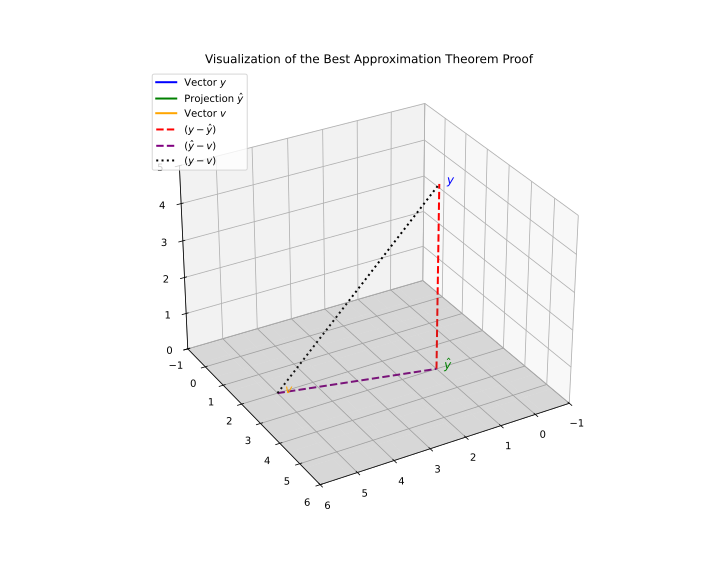
\includegraphics[keepaspectratio]{lec1-vecspace_files/figure-pdf/fig-3d-proof-1.pdf}}

}

\caption{\label{fig-3d-proof}Visualization of the Best Approximation
Theorem}

\end{figure}%

\subsection{Uniqueness of Projection}\label{uniqueness-of-projection}

While the existence of a least-squares solution is guaranteed, we must
also prove that there is only one such vector.

\begin{theorem}[Uniqueness of Orthogonal
Projection]\protect\hypertarget{thm-projection-uniqueness}{}\label{thm-projection-uniqueness}

For a given vector \(y\) and subspace \(V\), the projection vector
\(\hat{y}\) satisfying \((y - \hat{y}) \perp V\) is unique.

\end{theorem}

\begin{proof}
Assume there are two vectors \(\hat{y}_1 \in V\) and \(\hat{y}_2 \in V\)
that both satisfy the orthogonality condition. \[
(y - \hat{y}_1) \perp V \quad \text{and} \quad (y - \hat{y}_2) \perp V
\] This means that for any \(v \in V\), both inner products are zero: \[
\langle y - \hat{y}_1, v \rangle = 0
\] \[
\langle y - \hat{y}_2, v \rangle = 0
\]

Subtracting the second equation from the first:

\[
\langle y - \hat{y}_1, v \rangle - \langle y - \hat{y}_2, v \rangle = 0
\] Using the linearity of the inner product: \[
\langle (y - \hat{y}_1) - (y - \hat{y}_2), v \rangle = 0
\] \[
\langle \hat{y}_2 - \hat{y}_1, v \rangle = 0
\]

This equation holds for \textbf{all} \(v \in V\). Since \(\hat{y}_1\)
and \(\hat{y}_2\) are both in \(V\), their difference
\(d = \hat{y}_2 - \hat{y}_1\) must also be in \(V\). We can therefore
choose \(v = d = \hat{y}_2 - \hat{y}_1\).

\[
\langle \hat{y}_2 - \hat{y}_1, \hat{y}_2 - \hat{y}_1 \rangle = 0 \implies \|\hat{y}_2 - \hat{y}_1\|^2 = 0
\] The only vector with a norm of zero is the zero vector itself. \[
\hat{y}_2 - \hat{y}_1 = 0 \implies \hat{y}_1 = \hat{y}_2
\] Thus, the projection is unique.
\end{proof}

\section{\texorpdfstring{Projection via Orthonormal Basis
(\(Q\))}{Projection via Orthonormal Basis (Q)}}\label{projection-via-orthonormal-basis-q}

\subsection{Orthonomal Basis}\label{orthonomal-basis}

Before discussing projections onto general subspaces, we must formally
define the coordinate system of a subspace, known as a basis.

\begin{definition}[Basis]\protect\hypertarget{def-basis}{}\label{def-basis}

A set of vectors \(\{x_1, \dots, x_k\}\) is a \textbf{Basis} for a
vector space \(V\) if:

\begin{enumerate}
\def\labelenumi{\arabic{enumi}.}
\tightlist
\item
  The vectors span the space: \(V = L(x_1, \dots, x_k)\).
\item
  The vectors are linearly independent.
\end{enumerate}

\end{definition}

The number of vectors in a basis is unique and is defined as the
\textbf{Dimension} of \(V\).

Calculations become significantly simpler if we choose a basis with
special geometric properties.

\begin{definition}[Orthonormal
Basis]\protect\hypertarget{def-orthonormal-basis}{}\label{def-orthonormal-basis}

A basis \(\{q_1, \dots, q_k\}\) is called an \textbf{Orthonormal Basis}
if:

\begin{enumerate}
\def\labelenumi{\arabic{enumi}.}
\tightlist
\item
  \textbf{Orthogonal:} Each pair of vectors is perpendicular.
\end{enumerate}

\[
    q_i'q_j = 0 \quad \text{for } i \ne j
    \]

\begin{enumerate}
\def\labelenumi{\arabic{enumi}.}
\setcounter{enumi}{1}
\tightlist
\item
  \textbf{Normalized:} Each vector has unit length.
\end{enumerate}

\[
    ||q_i||^2 = q_i'q_i = 1
    \]

Combining these, we write \(q_i'q_j = \delta_{ij}\) (Kronecker delta).

\end{definition}

We now generalize the projection problem. Instead of projecting \(y\)
onto a single line, we project it onto a subspace \(V\) of dimension
\(k\).

If we have an orthonormal basis \(\{q_1, \dots, q_k\}\) for \(V\), the
projection \(\hat{y}\) is simply the sum of the projections onto the
individual basis vectors.

\begin{definition}[Projection Defined with Orthonormal
Basis]\protect\hypertarget{def-proj-orthonormal}{}\label{def-proj-orthonormal}

The projection of \(y\) onto the subspace \(V = L(q_1, \dots, q_k)\) is:
\[
\hat{y} = \sum_{i=1}^k \text{proj}(y|q_i) = \sum_{i=1}^k (q_i'y) q_i
\]

Since the basis vectors are normalized, we do not need to divide by
\(||q_i||^2\).

\end{definition}

\begin{theorem}[Projection via Orthonormal
Basis]\protect\hypertarget{thm-orthonormal-basis-proj}{}\label{thm-orthonormal-basis-proj}

Let \(\{q_1, \dots, q_k\}\) be an orthonormal basis for the subspace
\(V \subseteq \mathbb{R}^n\). The vector defined by the sum of
individual projections: \[
\hat{y} = \sum_{i=1}^k \langle y, q_i \rangle q_i
\] is indeed the orthogonal projection of \(y\) onto \(V\). That is, it
satisfies \((y - \hat{y}) \perp V\).

\end{theorem}

\begin{proof}
To prove this, we must check two conditions:

\begin{enumerate}
\def\labelenumi{\arabic{enumi}.}
\item
  \(\hat{y} \in V\): This is immediate because \(\hat{y}\) is a linear
  combination of the basis vectors \(\{q_1, \dots, q_k\}\).
\item
  \((y - \hat{y}) \perp V\): It suffices to show that the error vector
  \(e = y - \hat{y}\) is orthogonal to every basis vector \(q_j\) (for
  \(j = 1, \dots, k\)).

  Let's calculate the inner product
  \(\langle y - \hat{y}, q_j \rangle\):

  \[
  \begin{aligned}
  \langle y - \hat{y}, q_j \rangle &= \langle y, q_j \rangle - \langle \hat{y}, q_j \rangle \\
  &= \langle y, q_j \rangle - \left\langle \sum_{i=1}^k \langle y, q_i \rangle q_i, q_j \right\rangle \\
  &= \langle y, q_j \rangle - \sum_{i=1}^k \langle y, q_i \rangle \underbrace{\langle q_i, q_j \rangle}_{\delta_{ij}}
  \end{aligned}
  \]

  Since the basis is orthonormal, \(\langle q_i, q_j \rangle\) is 1 if
  \(i=j\) and 0 otherwise. Thus, the summation collapses to a single
  term where \(i=j\):

  \[
  \begin{aligned}
  \langle y - \hat{y}, q_j \rangle &= \langle y, q_j \rangle - \langle y, q_j \rangle \cdot 1 \\
  &= 0
  \end{aligned}
  \]

  Since \((y - \hat{y})\) is orthogonal to every basis vector \(q_j\),
  it is orthogonal to the entire subspace \(V\). Thus, \(\hat{y}\) is
  the unique orthogonal projection.
\end{enumerate}

\end{proof}

\subsection{\texorpdfstring{Projection Matrix via Orthonomal Basis
(\(Q\))}{Projection Matrix via Orthonomal Basis (Q)}}\label{projection-matrix-via-orthonomal-basis-q}

\textbf{Matrix Form with Orthonormal Basis}

We can express the summation formula for \(\hat{y}\) compactly using
matrix notation.

Let \(Q\) be an \(n \times k\) matrix whose columns are the orthonormal
basis vectors \(q_1, \dots, q_k\).

\[
Q = \begin{pmatrix} q_1 & q_2 & \dots & q_k \end{pmatrix}
\]

Properties of \(Q\):

\begin{itemize}
\tightlist
\item
  \(Q'Q = I_k\) (Identity matrix of size \(k \times k\)).
\item
  \(QQ'\) is \textbf{not} necessarily \(I_n\) (unless \(k=n\)).
\end{itemize}

\begin{definition}[Projection Matrix in Terms of
\(Q\)]\protect\hypertarget{def-proj-matrix-orthonormal}{}\label{def-proj-matrix-orthonormal}

The projection \(\hat{y}\) can be written as: \[
\hat{y} = \begin{pmatrix} q_1 & \dots & q_k \end{pmatrix} \begin{pmatrix} q_1'y \\ \vdots \\ q_k'y \end{pmatrix} = Q (Q'y) = (QQ') y
\]

Thus, the projection matrix \(P\) onto the subspace \(V\) is:

\[
P = QQ'
\]

\end{definition}

\textbf{Properties of Projection Matrices}

We have defined the projection matrix as \(P = X(X'X)^{-1}X'\) (or
\(P=QQ'\) for orthonormal bases). All orthogonal projection matrices
share two fundamental algebraic properties.

\begin{theorem}[Symmeticity and
Idempotence]\protect\hypertarget{thm-projection-properties}{}\label{thm-projection-properties}

A square matrix \(P\) represents an orthogonal projection onto some
subspace if and only if it satisfies:

\begin{enumerate}
\def\labelenumi{\arabic{enumi}.}
\tightlist
\item
  \textbf{Idempotence:} \(P^2 = P\) (Applying the projection twice is
  the same as applying it once).
\item
  \textbf{Symmetry:} \(P' = P\).
\end{enumerate}

\end{theorem}

\begin{proof}
If \(\hat{y} = Py\) is already in the subspace \(\text{Col}(X)\), then
projecting it again should not change it. \[
P(Py) = Py \implies P^2 y = Py \quad \forall y
\] Thus, \(P^2 = P\).
\end{proof}

\textbf{Example: ANOVA (Analysis of Variance)}

One of the most common applications of projection is in Analysis of
Variance (ANOVA). We can view the calculation of group means as a
projection onto a subspace defined by group indicator variables.

\begin{example}[Finding Projection for One-way
ANOVA]\protect\hypertarget{exm-anova-projection}{}\label{exm-anova-projection}

Consider a one-way ANOVA model with \(k\) groups: \[
y_{ij} = \mu_i + \epsilon_{ij}
\] where \(i \in \{1, \dots, k\}\) represents the group and
\(j \in \{1, \dots, n_i\}\) represents the observation within the group.
Let \(N = \sum_{i=1}^k n_i\) be the total number of observations.

\begin{enumerate}
\def\labelenumi{\arabic{enumi}.}
\item
  \textbf{Matrix Definitions}

  We define the data vector \(y\) and the design matrix \(X\) as
  follows:

  \begin{itemize}
  \tightlist
  \item
    \textbf{Data Vector} (\(y\)): An \(N \times 1\) vector containing
    all observations by group:
  \end{itemize}

  \[
      y = \begin{pmatrix} y_{11} \\ \vdots \\ y_{1n_1} \\ y_{21} \\ \vdots \\ y_{kn_k} \end{pmatrix}
      \]

  \begin{itemize}
  \tightlist
  \item
    \textbf{Design Matrix} (\(X\)): An \(N \times k\) matrix constructed
    from \(k\) column vectors, \(X = (x_1, x_2, \dots, x_k)\). Each
    vector \(x_g\) is an \textbf{indicator} (dummy variable) for group
    \(g\):
  \end{itemize}

  \[
      x_g = \begin{pmatrix} 0 \\ \vdots \\ 1 \\ \vdots \\ 0 \end{pmatrix} \quad \leftarrow \text{Entries are 1 if observation belongs to group } g
      \]
\item
  \textbf{Orthogonality}

  These column vectors \(x_1, \dots, x_k\) are mutually orthogonal
  because no observation can belong to two groups at once. The dot
  product of any two distinct columns is zero:

  \[
  \langle x_g, x_h \rangle = 0 \quad \text{for } g \neq h
  \] This allows us to find the projection onto the column space of
  \(X\) by simply summing the projections onto each column individually.
\item
  \textbf{Calculating Individual Projections}

  For a specific group vector \(x_g\), the projection is:

  \[
  \text{proj}(y|x_g) = \frac{\langle y, x_g \rangle}{\langle x_g, x_g \rangle} x_g
  \]

  We calculate the two scalar terms:

  \begin{itemize}
  \tightlist
  \item
    \textbf{Denominator} (\(\langle x_g, x_g \rangle\)): The sum of
    squared elements of \(x_g\). Since \(x_g\) contains \(n_g\) ones and
    zeros elsewhere:
  \end{itemize}

  \[
      \langle x_g, x_g \rangle = \sum \mathbb{1}_{\{i=g\}}^2 = n_g
      \]

  \begin{itemize}
  \tightlist
  \item
    \textbf{Numerator} (\(\langle y, x_g \rangle\)): The dot product
    sums only the \(y\) values belonging to group \(g\):
  \end{itemize}

  \[
      \langle y, x_g \rangle = \sum_{i,j} y_{ij} \cdot \mathbb{1}_{\{i=g\}} = \sum_{j=1}^{n_g} y_{gj} = y_{g.} \quad (\text{Group Total})
      \]
\item
  \textbf{The Resulting Projection}

  Substituting these back into the formula gives the coefficient for the
  vector \(x_g\):

  \[
  \text{proj}(y|x_g) = \frac{y_{g.}}{n_g} x_g = \bar{y}_{g.} x_g
  \]

  The total projection \(\hat{y}\) is the sum over all groups:

  \[
  \hat{y} = \sum_{g=1}^k \bar{y}_{g.} x_g
  \] This confirms that the fitted value for any specific observation
  \(y_{ij}\) is simply its group mean \(\bar{y}_{i.}\).
\end{enumerate}

\end{example}

\subsection{Gram-Schmidt Process}\label{gram-schmidt-process}

To use the simplified formula \(P = QQ'\), we need an orthonormal basis.
The Gram-Schmidt process provides a method to construct such a basis
from any set of linearly independent vectors.

\textbf{Gram-Schmidt Process} Given linearly independent vectors
\(x_1, \dots, x_p\):

\begin{enumerate}
\def\labelenumi{\arabic{enumi}.}
\tightlist
\item
  \textbf{Step 1:} Normalize the first vector.
\end{enumerate}

\[
    q_1 = \frac{x_1}{||x_1||}
    \]

\begin{enumerate}
\def\labelenumi{\arabic{enumi}.}
\setcounter{enumi}{1}
\tightlist
\item
  \textbf{Step 2:} Project \(x_2\) onto \(q_1\) and subtract it to find
  the orthogonal component.
\end{enumerate}

\[
    v_2 = x_2 - (x_2'q_1)q_1
    \] Then normalize: \[
    q_2 = \frac{v_2}{||v_2||}
    \]

\begin{enumerate}
\def\labelenumi{\arabic{enumi}.}
\setcounter{enumi}{2}
\tightlist
\item
  \textbf{Step k:} Subtract the projections onto all previous \(q\)
  vectors.
\end{enumerate}

\[
    v_k = x_k - \sum_{j=1}^{k-1} (x_k'q_j)q_j
    \] \[
    q_k = \frac{v_k}{||v_k||}
    \]

\begin{figure}

\centering{

\pandocbounded{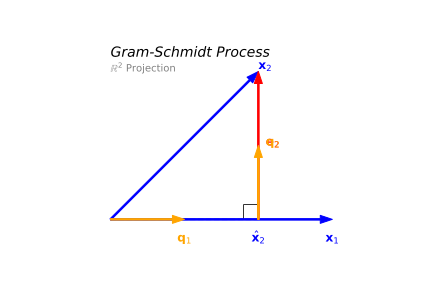
\includegraphics[keepaspectratio]{lec1-vecspace_files/figure-pdf/fig-gram-schmidt-python-3.pdf}}

}

\caption{\label{fig-gram-schmidt-python}Gram-Schmidt Process: Projecting
\(x_2\) onto \(x_1\)}

\end{figure}%

This process leads to the \textbf{QR Decomposition} of a matrix:
\(X = QR\), where \(Q\) is orthogonal and \(R\) is upper triangular.

\section{\texorpdfstring{Hat Matrix (Projection Matrix via
\(X\))}{Hat Matrix (Projection Matrix via X)}}\label{hat-matrix-projection-matrix-via-x}

\subsection{Norm Equations}\label{norm-equations}

Let \(X = (x_1, \dots, x_p)\) be an \(n \times p\) matrix, where each
column \(x_j\) is a predictor vector.

We want to project the target vector \(y\) onto the column space
\(\text{Col}(X)\). This is equivalent to finding a coefficient vector
\(\beta \in \mathbb{R}^p\) such that the error vector (residual) is
orthogonal to the entire subspace \(\text{Col}(X)\).

\[
y - X\beta \perp \text{Col}(X)
\]

Since the columns of \(X\) span the subspace, the residual must be
orthogonal to \textbf{every} column vector \(x_j\) individually:

\[
y - X\beta \perp x_j \quad \text{for } j = 1, \dots, p
\]

Writing this geometric condition as an algebraic dot product (where
\(x_j'\) denotes the transpose):

\[
x_j'(y - X\beta) = 0 \quad \text{for each } j
\]

We can stack these \(p\) separate linear equations into a single matrix
equation. Since the rows of \(X'\) are the columns of \(X\), this
becomes:

\[
\begin{pmatrix} x_1' \\ \vdots \\ x_p' \end{pmatrix} (y - X\beta) = \mathbf{0}
\implies X'(y - X\beta) = 0
\]

Finally, we distribute the matrix transpose and rearrange terms to solve
for \(\beta\):

\[
\begin{aligned}
X'y - X'X\beta &= 0 \\
X'X\beta &= X'y
\end{aligned}
\]

This system is known as the \textbf{Normal Equations}.

\begin{theorem}[Least Squares
Estimator]\protect\hypertarget{thm-least-squares-estimator}{}\label{thm-least-squares-estimator}

If \(X'X\) is invertible (i.e., \(X\) has full column rank), the unique
solution for \(\beta\) is: \[
\hat{\beta} = (X'X)^{-1}X'y
\]

\end{theorem}

\subsection{Hat Matrix}\label{hat-matrix}

Substituting the estimator \(\hat{\beta}\) back into the equation for
\(\hat{y}\) gives us the projection matrix.

\begin{definition}[Hat
Matrix]\protect\hypertarget{def-projection-matrix-general}{}\label{def-projection-matrix-general}

The projection of \(y\) onto \(\text{Col}(X)\) is given by: \[
\hat{y} = X\hat{\beta} = X(X'X)^{-1}X'y
\]

Thus, the hat matrix \(H\) is defined as:

\[
H = X(X'X)^{-1}X'
\]

\end{definition}

\subsection{\texorpdfstring{Equivalence of Hat Matrix and
\(QQ'\)}{Equivalence of Hat Matrix and QQ\textquotesingle{}}}\label{equivalence-of-hat-matrix-and-qq}

If we use the QR decomposition such that \(X = QR\), where the columns
of \(Q\) form an orthonormal basis for \(\text{Col}(X)\), the formula
simplifies significantly.

Recall that for orthonormal columns, \(Q'Q = I\). Substituting \(X=QR\)
into the general formula:

\[
\begin{aligned}
H &= QR((QR)'(QR))^{-1}(QR)' \\
  &= QR(R'Q'QR)^{-1}R'Q' \\
  &= QR(R' \underbrace{Q'Q}_{I} R)^{-1}R'Q' \\
  &= QR(R'R)^{-1}R'Q' \\
  &= QR R^{-1} (R')^{-1} R' Q' \\
  &= Q \underbrace{R R^{-1}}_{I} \underbrace{(R')^{-1} R'}_{I} Q' \\
  &= Q Q'
\end{aligned}
\]

This confirms that \(H = QQ'\) is consistent with the general formula
\(H = X(X'X)^{-1}X'\).

\subsection{Properties of Hat Matrix}\label{properties-of-hat-matrix}

We revisit the properties of projection matrices in this general
context.

\begin{theorem}[Properties of Hat
Matrix]\protect\hypertarget{thm-projection-properties-revisited}{}\label{thm-projection-properties-revisited}

The matrix \(H = X(X'X)^{-1}X'\) satisfies:

\begin{enumerate}
\def\labelenumi{\arabic{enumi}.}
\tightlist
\item
  \textbf{Symmetric:} \(H' = H\)
\item
  \textbf{Idempotent:} \(H^2 = H\)
\item
  \textbf{Trace:} The trace of a projection matrix equals the dimension
  of the subspace it projects onto. \[
  \text{tr}(H) = \text{tr}(X(X'X)^{-1}X') = \text{tr}((X'X)^{-1}X'X) = \text{tr}(I_p) = p
  \]
\end{enumerate}

\end{theorem}

\section{Projection Defined with Orthogonal Projection
Matrix}\label{projection-defined-with-orthogonal-projection-matrix}

Projection don't have to be defined with a subspace or a matrix \(X\) as
we discussed before. Projection matrix is a self-contained definition of
the subspace it projects onto.

\subsection{Orthogonal Projection
Matrix}\label{orthogonal-projection-matrix}

\begin{definition}[Orthogonal Projection
Matrix]\protect\hypertarget{def-proj-matrix}{}\label{def-proj-matrix}

A square matrix \(P\) is called an \textbf{orthogonal projection matrix}
if it satisfies two conditions:

\begin{enumerate}
\def\labelenumi{\arabic{enumi}.}
\tightlist
\item
  \textbf{Symmetry:} \(P^\top = P\)
\item
  \textbf{Idempotency:} \(P^2 = P\)
\end{enumerate}

\end{definition}

\begin{theorem}[Projection onto Column
Space]\protect\hypertarget{thm-proj-col}{}\label{thm-proj-col}

Let \(P\) be a \(p \times p\) symmetric (\(P^\top = P\)) and idempotent
(\(P^2 = P\)) matrix in \(\mathbb{R}^p\). Then \(P\) represents the
orthogonal projection onto its column space, \(\text{Col}(P)\).

Specifically, for any vector \(y \in \mathbb{R}^p\), the vector
\(\hat{y} = Py\) satisfies the definition of orthogonal projection:

\begin{enumerate}
\def\labelenumi{\arabic{enumi}.}
\tightlist
\item
  \(\hat{y} \in \text{Col}(P)\)
\item
  \(y - \hat{y} \perp \text{Col}(P)\)
\end{enumerate}

\end{theorem}

\begin{proof}
To prove that \(P\) is the orthogonal projector onto \(\text{Col}(P)\),
we verify the two conditions for an arbitrary vector
\(y \in \mathbb{R}^p\).

\begin{enumerate}
\def\labelenumi{\arabic{enumi}.}
\item
  Condition: \(\hat{y} \in \text{Col}(P)\)

  By the definition of matrix-vector multiplication, \(\hat{y} = Py\) is
  a linear combination of the columns of \(P\). Therefore, \(\hat{y}\)
  is, by definition, an element of \(\text{Col}(P)\).
\item
  Condition: \(y - \hat{y} \perp \text{Col}(P)\)

  Let \(e = y - \hat{y} = (I_n - P)y\). To verify that \(e\) is
  orthogonal to \(\text{Col}(P)\), it suffices to show that \(e\) is
  orthogonal to every column of \(P\). In matrix notation, this is
  equivalent to showing \(e^\top P = 0\). We compute this directly:
\end{enumerate}

\[
\begin{aligned}
e^\top P &= [(I_p - P)y]^\top P \\
&= y^\top (I_p - P)^\top P \\
&= y^\top (I_p - P) P & (\text{Symmetry: } P^\top = P) \\
&= y^\top (P - P^2) \\
&= y^\top (P - P) & (\text{Idempotency: } P^2 = P) \\
&= 0
\end{aligned}
\]

Since \(e^\top P = 0\), the residual \(e\) is orthogonal to every column
of \(P\). Consequently, \(e\) is orthogonal to the space spanned by
those columns, \(\text{Col}(P)\).
\end{proof}

\begin{lemma}[0-1
Projection]\protect\hypertarget{lem-projection-props}{}\label{lem-projection-props}

Let \(P\) be a \(n \times n\) matrix. \(P\) is the orthogonal projection
matrix onto \(\text{Col}(P)\) if and only if:

\begin{enumerate}
\def\labelenumi{\arabic{enumi})}
\tightlist
\item
  \(Pv = v\) for all \(v \in \text{Col}(P)\).
\item
  \(Pv = 0\) for all \(v \perp \text{Col}(P)\).
\end{enumerate}

\end{lemma}

\begin{proof}
\textbf{Forward Implication (\(\implies\)):} Given \(P\) is an
orthogonal projection (\(P^2=P, P^\top=P\)).

\begin{enumerate}
\def\labelenumi{(\arabic{enumi})}
\tightlist
\item
  \textbf{Proof of (1):} Let \(v \in \text{Col}(P)\). Then \(v = Px\)
  for some \(x\). \[
     Pv = P(Px) = P^2 x = Px = v
     \]
\item
  \textbf{Proof of (2):} Let \(v \perp \text{Col}(P)\). Then \(v\) is
  orthogonal to every column of \(P\), so \(v^\top P = 0\). Since \(P\)
  is symmetric:
\end{enumerate}

\[
   Pv = (v^\top P^\top)^\top = (v^\top P)^\top = 0^\top = 0
   \]

\textbf{Reverse Implication (\(\impliedby\)):} Given conditions (1) and
(2) hold.

We must show that \(P\) is idempotent (\(P^2=P\)) and symmetric
(\(P^\top=P\)).

\begin{enumerate}
\def\labelenumi{(\arabic{enumi})}
\item
  \textbf{Proof of Idempotence (\(P^2 = P\)):} For any vector
  \(x \in \mathbb{R}^n\), let \(y = Px\). By definition,
  \(y \in \text{Col}(P)\). Applying condition (1) to the vector \(y\):
  \[
     Py = y \implies P(Px) = Px \implies P^2 x = Px
     \] Since this holds for all \(x\), \(P^2 = P\).
\item
  \textbf{Proof of Symmetry (\(P^\top = P\)):} We decompose any two
  vectors \(x, y \in \mathbb{R}^n\) into components inside and
  orthogonal to \(\text{Col}(P)\). Let \(x = x_1 + x_2\) and
  \(y = y_1 + y_2\), where \(x_1, y_1 \in \text{Col}(P)\) and
  \(x_2, y_2 \perp \text{Col}(P)\). Using conditions (1) and (2): \[
     Px = P(x_1 + x_2) = Px_1 + Px_2 \stackrel{(1),(2)}{=} x_1 + 0 = x_1
     \]\\
  \[
     Py = P(y_1 + y_2) = Py_1 + Py_2 \stackrel{(1),(2)}{=} y_1 + 0 = y_1
     \] Now we compare the inner products \(\langle Px, y \rangle\) and
  \(\langle x, Py \rangle\): \[
     \langle Px, y \rangle = \langle x_1, y_1 + y_2 \rangle = \langle x_1, y_1 \rangle + \underbrace{\langle x_1, y_2 \rangle}_{0} = \langle x_1, y_1 \rangle
     \]
\end{enumerate}

\[
   \langle x, Py \rangle = \langle x_1 + x_2, y_1 \rangle = \langle x_1, y_1 \rangle + \underbrace{\langle x_2, y_1 \rangle}_{0} = \langle x_1, y_1 \rangle
   \] Since \(\langle Px, y \rangle = \langle x, Py \rangle\) implies
\(x^\top P^\top y = x^\top P y\) for all \(x, y\), we conclude
\(P^\top = P\).

Since \(P\) is symmetric and idempotent, it is the orthogonal projection
matrix.
\end{proof}

\subsection{Projection onto Complement
Space}\label{projection-onto-complement-space}

\begin{theorem}[Projection onto Orthogonal
Complement]\protect\hypertarget{thm-complement-proj}{}\label{thm-complement-proj}

Let \(P\) be a \(n \times n\) orthogonal projection matrix operating in
the space \(\mathbb{R}^n\). The matrix \(M\) defined as: \[
M = I_p - P
\] is the orthogonal projection matrix onto the orthogonal complement of
the column space of \(P\), denoted
\(\text{Col}(P)^\perp \subseteq \mathbb{R}^n\).

\end{theorem}

\begin{proof}
\leavevmode

\begin{enumerate}
\def\labelenumi{(\arabic{enumi})}
\item
  \textbf{Symmetry and Idempotency} Since \(P\) is a projection matrix,
  \(P^\top = P\) and \(P^2 = P\). We verify these properties for \(M\):
  \begin{equation}\phantomsection\label{eq-m-sym}{
     M^\top = (I_p - P)^\top = I_p - P^\top = I_p - P = M
     }\end{equation} \begin{equation}\phantomsection\label{eq-m-idemp}{
     M^2 = (I_p - P)(I_p - P) = I_p - 2P + P^2 = I_p - 2P + P = I_p - P = M
     }\end{equation} By Equation~\ref{eq-m-sym} and
  Equation~\ref{eq-m-idemp}, \(M\) is symmetric and idempotent, so it is
  an orthogonal projection matrix.
\item
  \textbf{Identifying the Subspace} We now show that
  \(\text{Col}(M) = \text{Col}(P)^\perp\) by mutual inclusion.

  \begin{enumerate}
  \def\labelenumii{(\arabic{enumii})}
  \item
    \textbf{Direction 1}:
    \(\text{Col}(M) \subseteq \text{Col}(P)^\perp\) Let
    \(v \in \text{Col}(M)\). Then \(v = Mx\) for some vector \(x\).
    Multiplying by \(P\): \[
      Pv = P(I_p - P)x = (P - P^2)x = 0
      \] Since \(P\) is symmetric (\(P = P'\)), taking the transpose of
    \(Pv=0\) gives \(v'P = 0\). This means \(v\) is orthogonal to every
    column of \(P\). Therefore, \(v \in \text{Col}(P)^\perp\).
  \item
    \textbf{Direction 2}:
    \(\text{Col}(P)^\perp \subseteq \text{Col}(M)\) Let
    \(v \in \text{Col}(P)^\perp\). By definition, \(v\) is orthogonal to
    the columns of \(P\), so \(v'P = 0\). Taking the transpose and using
    symmetry (\(P' = P\)), we get \(Pv = 0\).\\
    Now applying \(M\) to \(v\): \[
      Mv = (I_p - P)v = v - Pv = v
      \] Since \(Mv = v\), \(v\) lies in the column space of \(M\).
    Therefore, \(v \in \text{Col}(M)\).
  \end{enumerate}
\end{enumerate}

Since both inclusions hold, \(\text{Col}(M) = \text{Col}(P)^\perp\).
\end{proof}

\subsection{Projections onto Nested
Subspaces}\label{projections-onto-nested-subspaces}

\subsubsection{Iterative Projections}\label{iterative-projections}

\begin{theorem}[Iterative
Projections]\protect\hypertarget{thm-nested-projections}{}\label{thm-nested-projections}

Let \(P_0\) and \(P_1\) be \(n \times n\) orthogonal projection matrices
such that \(\text{Col}(P_0) \subseteq \text{Col}(P_1)\). Then:

\begin{enumerate}
\def\labelenumi{(\arabic{enumi})}
\tightlist
\item
  \(P_1 P_0 = P_0\)
\item
  \(P_0 P_1 = P_0\)
\end{enumerate}

\end{theorem}

\begin{proof}
\textbf{Method 1}:

Proof of \(P_1 P_0 = P_0\):

Let \(y \in \mathbb{R}^n\) be an arbitrary vector. By definition, the
vector \(v = P_0 y\) lies in \(\text{Col}(P_0)\). Given
\(\text{Col}(P_0) \subseteq \text{Col}(P_1)\), it follows that
\(v \in \text{Col}(P_1)\).

Using \textbf{Lemma Lemma~\ref{lem-projection-props}}, since
\(v \in \text{Col}(P_1)\), \(P_1\) acts as the identity on \(v\), so
\(P_1 v = v\). Substituting \(v = P_0 y\):

\[
P_1 (P_0 y) = P_0 y
\]

Since \(P_1 P_0 y = P_0 y\) holds for all \(y \in \mathbb{R}^n\), we
conclude \(P_1 P_0 = P_0\).

Proof of \(P_0 P_1 = P_0\):

Taking the transpose of the result from part 1 and applying the symmetry
property (\(P' = P\)):

\[
(P_1 P_0)' = P_0' \implies P_0' P_1' = P_0' \implies P_0 P_1 = P_0
\]

\textbf{Method 2}:

To prove \(P_0 P_1 = P_0\), for any \(y \in \mathbb{R}^n\), let
\(\hat{y}_1 = P_1 y\), \(\hat{y}_0 = P_0 y\), \(e_1 = y - \hat{y}_1\),
and \(e_0 = y - \hat{y}_0\). Note that both \(e_0\) and \(e_1\) are
orthogonal to \(\text{Col}(P_0)\) (since
\(\text{Col}(P_0) \subseteq \text{Col}(P_1)\)).

We have:

\[
P_0(P_1 - P_0)y = P_0(\hat{y}_1 - \hat{y}_0) = P_0 (e_0 - e_1) = 0
\]

This implies \(P_0 P_1 - P_0 = 0\), so \(P_0 P_1 = P_0\).
\end{proof}

\subsubsection{Difference of
Projections}\label{difference-of-projections}

\begin{theorem}[Difference
Projection]\protect\hypertarget{thm-diff-projection}{}\label{thm-diff-projection}

The matrix \(P_{\Delta} = P_1 - P_0\) is an orthogonal projection matrix
onto the subspace \(\text{Col}(P_1) \cap \text{Col}(P_0)^\perp\). This
subspace represents the ``extra'' information in the full model that is
orthogonal to the reduced model. Additionally, the following column
space relationship holds: \[
\text{Col}(P_1 - P_0) = \text{Col}(P_0)^\perp \cap \text{Col}(P_1)
\]

\end{theorem}

\begin{proof}
\leavevmode

\begin{enumerate}
\def\labelenumi{\arabic{enumi}.}
\tightlist
\item
  \textbf{Symmetry:} Since \(P_1\) and \(P_0\) are symmetric:
\end{enumerate}

\[
(P_1 - P_0)' = P_1' - P_0' = P_1 - P_0
\]

\begin{enumerate}
\def\labelenumi{\arabic{enumi}.}
\setcounter{enumi}{1}
\tightlist
\item
  \textbf{Idempotency:}
\end{enumerate}

\[
\begin{aligned}
(P_1 - P_0)^2 &= (P_1 - P_0)(P_1 - P_0) \\
&= P_1^2 - P_1 P_0 - P_0 P_1 + P_0^2
\end{aligned}
\] Using the projection property (\(P^2=P\)) and the nested property
(\(P_1 P_0 = P_0\) and \(P_0 P_1 = P_0\)): \[
= P_1 - P_0 - P_0 + P_0 = P_1 - P_0
\]

\begin{enumerate}
\def\labelenumi{\arabic{enumi}.}
\setcounter{enumi}{2}
\tightlist
\item
  \textbf{Orthogonality to \(P_0\):}
\end{enumerate}

\[
(P_1 - P_0)P_0 = P_1 P_0 - P_0^2 = P_0 - P_0 = 0
\]

\begin{enumerate}
\def\labelenumi{\arabic{enumi}.}
\setcounter{enumi}{3}
\item
  \textbf{Column Space Identity:} We show
  \(\text{Col}(P_1 - P_0) = \text{Col}(P_0)^\perp \cap \text{Col}(P_1)\)
  via double containment.

  \textbf{\((\subseteq)\) Forward Containment:} Let
  \(y \in \text{Col}(P_1 - P_0)\). By definition, \(y = (P_1 - P_0)x\)
  for some \(x\).

  \begin{itemize}
  \tightlist
  \item
    Check \(y \in \text{Col}(P_1)\):
    \(P_1 y = P_1(P_1 - P_0)x = (P_1 - P_0)x = y\). Thus
    \(y \in \text{Col}(P_1)\).
  \item
    Check \(y \in \text{Col}(P_0)^\perp\):
    \(P_0 y = P_0(P_1 - P_0)x = (P_0 - P_0)x = 0\). Thus
    \(y \in \text{Col}(P_0)^\perp\).
  \item
    Therefore,
    \(\text{Col}(P_1 - P_0) \subseteq \text{Col}(P_0)^\perp \cap \text{Col}(P_1)\).
  \end{itemize}

  \textbf{\((\supseteq)\) Reverse Containment}: Let
  \(y \in \text{Col}(P_0)^\perp \cap \text{Col}(P_1)\).

  \begin{itemize}
  \tightlist
  \item
    Since \(y \in \text{Col}(P_1)\), \(P_1 y = y\).
  \item
    Since \(y \in \text{Col}(P_0)^\perp\), \(P_0 y = 0\).
  \item
    Observe \((P_1 - P_0)y = P_1 y - P_0 y = y - 0 = y\).
  \item
    This implies \(y\) is in the range of \((P_1 - P_0)\). Therefore,
    \(\text{Col}(P_0)^\perp \cap \text{Col}(P_1) \subseteq \text{Col}(P_1 - P_0)\).
  \end{itemize}
\end{enumerate}

\end{proof}

\begin{tcolorbox}[enhanced jigsaw, toprule=.15mm, titlerule=0mm, left=2mm, bottomrule=.15mm, opacityback=0, colback=white, leftrule=.75mm, coltitle=black, colbacktitle=quarto-callout-important-color!10!white, colframe=quarto-callout-important-color-frame, arc=.35mm, rightrule=.15mm, breakable, bottomtitle=1mm, toptitle=1mm, title=\textcolor{quarto-callout-important-color}{\faExclamation}\hspace{0.5em}{Important}, opacitybacktitle=0.6]

This is important as we can use \(P_2-P_1\) to construct the projection
matrix and the space that it projects onto.

\end{tcolorbox}

\textbf{Hat Matrix of Incremental Space}

\begin{theorem}[Hat Matrix of Incremental
Space]\protect\hypertarget{thm-hat-matrix-incremental}{}\label{thm-hat-matrix-incremental}

Let \(X_1\) be a design matrix of dimension \(n \times k_1\) and \(X_2\)
be a design matrix of dimension \(n \times k_2\), such that the combined
matrix \(X = [X_1, X_2]\) has full column rank. Let
\(V_1 = \text{Col}(X_1)\) and \(V_2 = \text{Col}([X_1, X_2])\). Let
\(P_1\) and \(P_2\) be the orthogonal projection matrices onto \(V_1\)
and \(V_2\), respectively.

Define the matrix of residuals \(\tilde{X}_2\) as:

\[
\tilde{X}_2 = (I - P_1) X_2
\]

Let \(W = \text{Col}(\tilde{X}_2)\). Let \(P_W\) be the \(n \times n\)
projection matrix onto \(W\), which is the hat matrix constructed from
\(\tilde{X}_2\):

\[
P_W = \tilde{X}_2 (\tilde{X}_2^T \tilde{X}_2)^{-1} \tilde{X}_2^T
\]

\begin{enumerate}
\def\labelenumi{(\alph{enumi})}
\tightlist
\item
  Let \(X^* = [X_1, \tilde{X}_2]\). Prove that the column space of the
  original design matrix \(X\) is identical to the column space of the
  modified design matrix \(X^*\):
\end{enumerate}

\[
\text{Col}([X_1, X_2]) = \text{Col}([X_1, \tilde{X}_2])
\]

\begin{enumerate}
\def\labelenumi{(\alph{enumi})}
\setcounter{enumi}{1}
\tightlist
\item
  Using the result from Part (a) and the definition of the Hat Matrix,
  prove that:
\end{enumerate}

\[
P_W = P_2 - P_1
\]

\end{theorem}

\begin{proof}
Assignment question.
\end{proof}

\subsection{Projection onto Three Multually Orthogonal
Subspaces}\label{projection-onto-three-multually-orthogonal-subspaces}

\begin{theorem}[Orthogonal
Decomposition]\protect\hypertarget{thm-nested-decomposition}{}\label{thm-nested-decomposition}

Let \(M_0 \subset M_1\) be two nested linear models associated with
orthogonal projection matrices \(P_0\) and \(P_1\), such that
\(\text{Col}(P_0) \subset \text{Col}(P_1)\).

For any observation vector \(y\), we have the decomposition:

\[
y = \underbrace{P_0 y}_{\hat{y}_0} + \underbrace{(P_1 - P_0) y}_{\hat{y}_1 - \hat{y}_0} + \underbrace{(I - P_1) y}_{y - \hat{y}_1}
\]

\textbf{Geometric Interpretation:}

\begin{enumerate}
\def\labelenumi{\arabic{enumi}.}
\tightlist
\item
  \(\hat{y}_0 \in \text{Col}(P_0)\): The fit of the reduced model.
\item
  \((\hat{y}_1 - \hat{y}_0) \in \text{Col}(P_0)^\perp \cap \text{Col}(P_1)\):
  The additional fit provided by \(M_1\) over \(M_0\).
\item
  \((y - \hat{y}_1) \in \text{Col}(P_1)^\perp\): The projection of \(y\)
  onto the \textbf{orthogonal complement} of \(\text{Col}(P_1)\).
\end{enumerate}

The three component vectors are mutually orthogonal. Consequently, their
squared norms sum to the total squared norm:

\[
\|y\|^2 = \|\hat{y}_0\|^2 + \|\hat{y}_1 - \hat{y}_0\|^2 + \|y - \hat{y}_1\|^2
\]

\end{theorem}

\begin{theorem}[Orthogonal
Decomposition]\protect\hypertarget{thm-nested-decomposition}{}\label{thm-nested-decomposition}

Let \(M_0 \subset M_1\) be two nested linear models associated with
orthogonal projection matrices \(P_0\) and \(P_1\), such that
\(\text{Col}(P_0) \subset \text{Col}(P_1)\).

For any observation vector \(y\), we have the decomposition:

\[
y = \underbrace{P_0 y}_{\hat{y}_0} + \underbrace{(P_1 - P_0) y}_{\hat{y}_1 - \hat{y}_0} + \underbrace{(I - P_1) y}_{y - \hat{y}_1}
\]

\textbf{Geometric Interpretation:}

\begin{enumerate}
\def\labelenumi{\arabic{enumi}.}
\tightlist
\item
  \(\hat{y}_0 \in \text{Col}(P_0)\): The fit of the reduced model.
\item
  \((\hat{y}_1 - \hat{y}_0) \in \text{Col}(P_0)^\perp \cap \text{Col}(P_1)\):
  The additional fit provided by \(M_1\) over \(M_0\).
\item
  \((y - \hat{y}_1) \in \text{Col}(P_1)^\perp\): The projection of \(y\)
  onto the \textbf{orthogonal complement} of \(\text{Col}(P_1)\).
\end{enumerate}

The three component vectors are mutually orthogonal. Consequently, their
squared norms sum to the total squared norm:

\[
\|y\|^2 = \|\hat{y}_0\|^2 + \|\hat{y}_1 - \hat{y}_0\|^2 + \|y - \hat{y}_1\|^2
\]

\end{theorem}

\begin{proof}
\leavevmode

\begin{enumerate}
\def\labelenumi{\arabic{enumi}.}
\item
  \textbf{Definition of Vectors and Nested Spaces}

  Let \(I\) be the identity matrix, which is the orthogonal projection
  onto the entire space \(\mathbb{R}^n\). We effectively have a
  three-level nested sequence of subspaces:

  \[
  \text{Col}(P_0) \subset \text{Col}(P_1) \subset \mathbb{R}^n
  \] We define the components of the decomposition using successive
  difference projections:

  \begin{itemize}
  \tightlist
  \item
    \(v_0 = P_0 y\)
  \item
    \(v_1 = (P_1 - P_0) y\)
  \item
    \(v_2 = (I - P_1) y\)
  \end{itemize}

  Summing these gives the identity: \(y = v_0 + v_1 + v_2\).
\item
  \textbf{Sequential Orthogonality via
  Theorem~\ref{thm-diff-projection}}

  We apply the Difference Projection Theorem
  (Theorem~\ref{thm-diff-projection}) to each successive pair of nested
  spaces to establish orthogonality.

  \begin{itemize}
  \tightlist
  \item
    \textbf{Step 1: Verify \(v_1 \perp v_0\)}

    \begin{itemize}
    \tightlist
    \item
      Consider the nested pair \(P_0\) and \(P_1\).
    \item
      By Theorem~\ref{thm-diff-projection}, the matrix \((P_1 - P_0)\)
      projects onto \(\text{Col}(P_0)^\perp \cap \text{Col}(P_1)\).
    \item
      Since \(v_0 \in \text{Col}(P_0)\) and \(v_1\) lies in the
      orthogonal complement \(\text{Col}(P_0)^\perp\), we have
      \textbf{\(v_1 \perp v_0\)}.
    \end{itemize}
  \item
    \textbf{Step 2: Verify \(v_2 \perp \{v_0, v_1\}\)}

    \begin{itemize}
    \tightlist
    \item
      Consider the nested pair \(P_1\) and \(I\) (where \(I\) projects
      onto \(\mathbb{R}^n\)).
    \item
      By Theorem~\ref{thm-diff-projection}, the matrix \((I - P_1)\)
      projects onto
      \(\text{Col}(P_1)^\perp \cap \mathbb{R}^n = \text{Col}(P_1)^\perp\).
    \item
      Since both \(v_0\) and \(v_1\) reside within \(\text{Col}(P_1)\)
      (as shown in Step 1), and \(v_2\) lies in the orthogonal
      complement \(\text{Col}(P_1)^\perp\), it follows that \(v_2\) is
      orthogonal to the entire subspace \(\text{Col}(P_1)\).
    \item
      Therefore, \textbf{\(v_2 \perp v_0\)} and
      \textbf{\(v_2 \perp v_1\)}.
    \end{itemize}
  \end{itemize}
\item
  \textbf{Conclusion}

  Since \(\{v_0, v_1, v_2\}\) are mutually orthogonal, the Pythagorean
  theorem applies:

  \[
  \|y\|^2 = \|v_0\|^2 + \|v_1\|^2 + \|v_2\|^2
  \] Substituting the original definitions back in: \[
  \|y\|^2 = \|\hat{y}_0\|^2 + \|\hat{y}_1 - \hat{y}_0\|^2 + \|y - \hat{y}_1\|^2
  \]
\end{enumerate}

\end{proof}

\begin{figure}[H]

\centering{

\pandocbounded{\includegraphics[keepaspectratio]{lec1-vecspace_files/figure-pdf/fig-anova-decomp-1.pdf}}

}

\caption{\label{fig-anova-decomp}Illustration of Projections onto Nested
Subspaces}

\end{figure}%

\begin{example}[ANOVA Sum
Squares]\protect\hypertarget{exm-anova-ss}{}\label{exm-anova-ss}

We apply the \textbf{Nested Model Theorem} (\(M_0 \subset M_1\)) to the
One-way ANOVA setting.

\begin{enumerate}
\def\labelenumi{\arabic{enumi}.}
\item
  Notation and Definitions

  Consider a dataset with \(k\) groups. Let \(i = 1, \dots, k\) index
  the groups, and \(j = 1, \dots, n_i\) index the observations within
  group \(i\).

  \begin{itemize}
  \item
    \(N\): Total number of observations, \(N = \sum_{i=1}^k n_i\).
  \item
    \(y_{ij}\): The \(j\)-th observation in the \(i\)-th group.
  \item
    \(\bar{y}_{i.}\): The sample mean of group \(i\).
  \end{itemize}

  \[ \bar{y}_{i.} = \frac{1}{n_i} \sum_{j=1}^{n_i} y_{ij} \]

  \begin{itemize}
  \tightlist
  \item
    \(\bar{y}_{..}\): The grand mean of all observations.
  \end{itemize}

  \[ \bar{y}_{..} = \frac{1}{N} \sum_{i=1}^k \sum_{j=1}^{n_i} y_{ij} \]
\item
  The Data and Projection Vectors

  \begin{longtable}[]{@{}
    >{\centering\arraybackslash}p{(\linewidth - 4\tabcolsep) * \real{0.3333}}
    >{\centering\arraybackslash}p{(\linewidth - 4\tabcolsep) * \real{0.3333}}
    >{\centering\arraybackslash}p{(\linewidth - 4\tabcolsep) * \real{0.3333}}@{}}
  \caption{ANOVA Vectors: Data, Null Model, and Full
  Model}\label{tbl-anova-vectors}\tabularnewline
  \toprule\noalign{}
  \begin{minipage}[b]{\linewidth}\centering
  Observation (\(y\))
  \end{minipage} & \begin{minipage}[b]{\linewidth}\centering
  Null Projection (\(\hat{y}_0\))
  \end{minipage} & \begin{minipage}[b]{\linewidth}\centering
  Full Projection (\(\hat{y}_1\))
  \end{minipage} \\
  \midrule\noalign{}
  \endfirsthead
  \toprule\noalign{}
  \begin{minipage}[b]{\linewidth}\centering
  Observation (\(y\))
  \end{minipage} & \begin{minipage}[b]{\linewidth}\centering
  Null Projection (\(\hat{y}_0\))
  \end{minipage} & \begin{minipage}[b]{\linewidth}\centering
  Full Projection (\(\hat{y}_1\))
  \end{minipage} \\
  \midrule\noalign{}
  \endhead
  \bottomrule\noalign{}
  \endlastfoot
  \(\begin{pmatrix} y_{11} \\ \vdots \\ y_{1 n_1} \\ \hline \vdots \\ \hline y_{k1} \\ \vdots \\ y_{k n_k} \end{pmatrix}\)
  &
  \(\begin{pmatrix} \bar{y}_{..} \\ \vdots \\ \bar{y}_{..} \\ \hline \vdots \\ \hline \bar{y}_{..} \\ \vdots \\ \bar{y}_{..} \end{pmatrix}\)
  &
  \(\begin{pmatrix} \bar{y}_{1.} \\ \vdots \\ \bar{y}_{1.} \\ \hline \vdots \\ \hline \bar{y}_{k.} \\ \vdots \\ \bar{y}_{k.} \end{pmatrix}\) \\
  \end{longtable}

  \begin{enumerate}
  \def\labelenumii{\arabic{enumii}.}
  \setcounter{enumii}{2}
  \tightlist
  \item
    Decomposition and Sum of Squares
  \end{enumerate}

  \begin{longtable}[]{@{}
    >{\raggedright\arraybackslash}p{(\linewidth - 8\tabcolsep) * \real{0.1918}}
    >{\centering\arraybackslash}p{(\linewidth - 8\tabcolsep) * \real{0.1918}}
    >{\centering\arraybackslash}p{(\linewidth - 8\tabcolsep) * \real{0.1918}}
    >{\raggedright\arraybackslash}p{(\linewidth - 8\tabcolsep) * \real{0.1918}}
    >{\raggedright\arraybackslash}p{(\linewidth - 8\tabcolsep) * \real{0.2329}}@{}}
  \toprule\noalign{}
  \begin{minipage}[b]{\linewidth}\raggedright
  Component
  \end{minipage} & \begin{minipage}[b]{\linewidth}\centering
  Notation
  \end{minipage} & \begin{minipage}[b]{\linewidth}\centering
  Definition
  \end{minipage} & \begin{minipage}[b]{\linewidth}\raggedright
  Vector Elements
  \end{minipage} & \begin{minipage}[b]{\linewidth}\raggedright
  Squared Norm (Sum of Squares)
  \end{minipage} \\
  \midrule\noalign{}
  \endhead
  \bottomrule\noalign{}
  \endlastfoot
  \textbf{Null Proj.} & \(\hat{y}_0\) & \(P_0 y\) & Grand Mean
  (\(\bar{y}_{..}\)) & \(\|\hat{y}_0\|^2 = N \bar{y}_{..}^2\) \\
  \textbf{Full Proj.} & \(\hat{y}_1\) & \(P_1 y\) & Group Means
  (\(\bar{y}_{i.}\)) &
  \(\|\hat{y}_1\|^2 = \sum_{i=1}^k n_i \bar{y}_{i.}^2\) \\
  \end{longtable}
\item
  Geometric Justification of Shortcut Formulas

  \textbf{A. Total Sum of Squares (SST)} Since
  \(\hat{y}_0 \perp (y - \hat{y}_0)\), we have
  \(\|y\|^2 = \|\hat{y}_0\|^2 + \|y - \hat{y}_0\|^2\):

  \[ \text{SST} = \|y - \hat{y}_0\|^2 = \|y\|^2 - \|\hat{y}_0\|^2 \]
  \[ \text{SST} = \sum_{i=1}^k \sum_{j=1}^{n_i} y_{ij}^2 - N\bar{y}_{..}^2 \]

  \textbf{B. Between Group Sum of Squares (SSB)} Since
  \(\hat{y}_0 \perp (\hat{y}_1 - \hat{y}_0)\), we have
  \(\|\hat{y}_1\|^2 = \|\hat{y}_0\|^2 + \|\hat{y}_1 - \hat{y}_0\|^2\):

  \[ \text{SSB} = \|\hat{y}_1 - \hat{y}_0\|^2 = \|\hat{y}_1\|^2 - \|\hat{y}_0\|^2 \]
  \[ \text{SSB} = \sum_{i=1}^k n_i\bar{y}_{i.}^2 - N\bar{y}_{..}^2 \]

  \textbf{C. Within Group Sum of Squares (SSW)} Since
  \(\hat{y}_1 \perp (y - \hat{y}_1)\), we have
  \(\|y\|^2 = \|\hat{y}_1\|^2 + \|y - \hat{y}_1\|^2\):

  \[ \text{SSW} = \|y - \hat{y}_1\|^2 = \|y\|^2 - \|\hat{y}_1\|^2 \]
  \[ \text{SSW} = \sum_{i=1}^k \sum_{j=1}^{n_i} y_{ij}^2 - \sum_{i=1}^k n_i\bar{y}_{i.}^2 \]

  \textbf{Conclusion:}

  \[ \underbrace{\|y\|^2 - N\bar{y}_{..}^2}_{\text{SST}} = \underbrace{(\sum n_i\bar{y}_{i.}^2 - N\bar{y}_{..}^2)}_{\text{SSB}} + \underbrace{(\sum \sum y_{ij}^2 - \sum n_i\bar{y}_{i.}^2)}_{\text{SSW}} \]
\item
  Visualizing ANOVA Components in Data Space
\end{enumerate}

\end{example}

\begin{figure}

\centering{

\pandocbounded{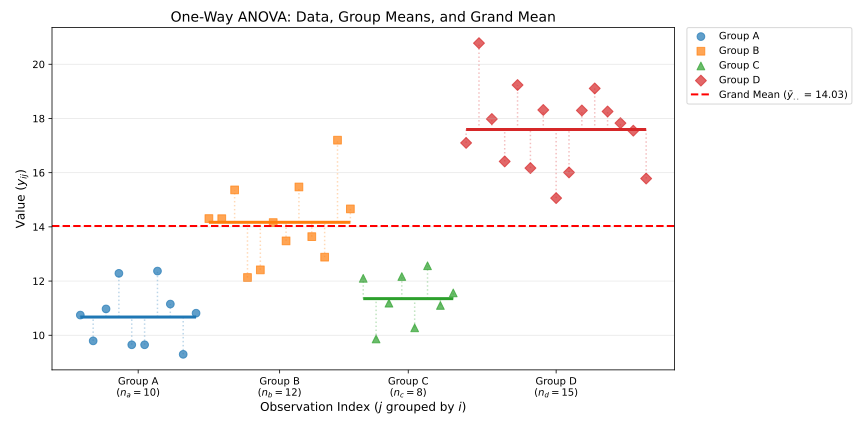
\includegraphics[keepaspectratio]{lec1-vecspace_files/figure-pdf/fig-anova-data-space-colored-7.pdf}}

}

\caption{\label{fig-anova-data-space-colored}Visualization of Group
Means vs.~Grand Mean}

\end{figure}%

\section{Projections onto More than Three Orthogonal
Subspaces}\label{projections-onto-more-than-three-orthogonal-subspaces}

Finally, we consider the case where the entire space \(\mathbb{R}^n\) is
decomposed into mutually orthogonal subspaces.

\begin{theorem}[General Orthogonal
Projections]\protect\hypertarget{thm-orth-decomposition}{}\label{thm-orth-decomposition}

If \(\mathbb{R}^n\) is the direct sum of orthogonal subspaces
\(V_1, V_2, \dots, V_k\): \[
\mathbb{R}^n = V_1 \oplus V_2 \oplus \dots \oplus V_k
\] where \(V_i \perp V_j\) for all \(i \ne j\).

Then any vector \(y\) can be uniquely written as:

\[
y = \hat{y}_1 + \hat{y}_2 + \dots + \hat{y}_k
\] where \(\hat{y}_i \in V_i\).

Furthermore, each component \(\hat{y}_i\) is simply the projection of
\(y\) onto the subspace \(V_i\):

\[
\hat{y}_i = P_i y
\]

\end{theorem}

\begin{proof}
\leavevmode

\begin{enumerate}
\def\labelenumi{\arabic{enumi}.}
\item
  Existence: Since \(\mathbb{R}^n\) is the direct sum of
  \(V_1, \dots, V_k\), by definition, any vector \(y \in \mathbb{R}^n\)
  can be written as a sum \(y = v_1 + \dots + v_k\) where
  \(v_i \in V_i\).
\item
  Uniqueness: Suppose there are two such representations:
  \(y = \sum v_i = \sum w_i\), with \(v_i, w_i \in V_i\). Then
  \(\sum (v_i - w_i) = 0\). Since subspaces in a direct sum are
  independent, the only way for the sum of elements to be zero is if
  each individual element is zero. Thus,
  \(v_i - w_i = 0 \implies v_i = w_i\). The representation is unique.
  Let \(\hat{y}_i = v_i\).
\item
  Projection Property: We claim that the \(i\)-th component
  \(\hat{y}_i\) is the orthogonal projection of \(y\) onto \(V_i\). We
  must show that the residual \((y - \hat{y}_i)\) is orthogonal to
  \(V_i\).

  \[
   y - \hat{y}_i = \sum_{j \ne i} \hat{y}_j
   \] Let \(z\) be any vector in \(V_i\). We calculate the inner
  product: \[
   \langle y - \hat{y}_i, z \rangle = \left\langle \sum_{j \ne i} \hat{y}_j, z \right\rangle = \sum_{j \ne i} \langle \hat{y}_j, z \rangle
   \] Since \(\hat{y}_j \in V_j\) and \(z \in V_i\), and the subspaces
  are mutually orthogonal (\(V_j \perp V_i\) for \(j \ne i\)), every
  term in the sum is zero. Therefore, \((y - \hat{y}_i) \perp V_i\). By
  the definition of orthogonal projection, \(\hat{y}_i = P_i y\).
\end{enumerate}

\end{proof}

This implies that the identity matrix can be decomposed into a sum of
projection matrices: \[
I_n = P_1 + P_2 + \dots + P_k
\]

\begin{figure}

\centering{

\pandocbounded{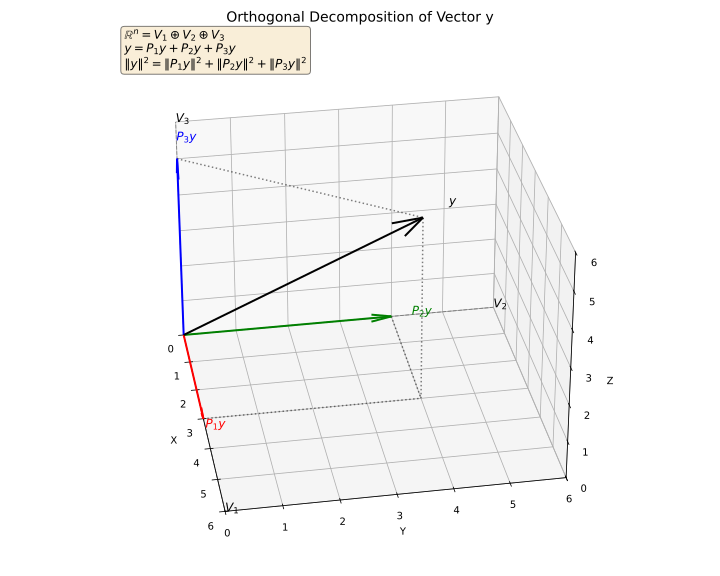
\includegraphics[keepaspectratio]{lec1-vecspace_files/figure-pdf/fig-orthogonal-decomp-rotated-9.pdf}}

}

\caption{\label{fig-orthogonal-decomp-rotated}Orthogonal decomposition
of vector y into subspaces}

\end{figure}%

\begin{theorem}[Complete Orthogonal Decomposition of
\(\mathbb{R}^n\)]\protect\hypertarget{thm-complete-decomposition}{}\label{thm-complete-decomposition}

Let \(P_0, P_1, \dots, P_k\) be a sequence of orthogonal projection
matrices with nested column spaces: \[
\text{Col}(P_0) \subseteq \text{Col}(P_1) \subseteq \dots \subseteq \text{Col}(P_k)
\]

Define the sequence of difference matrices \(\Delta P_i\) and their
column spaces \(V_i\) as follows:

\begin{align*}
\Delta P_0 &= P_0, & V_0 &= \text{Col}(\Delta P_0) \\
\Delta P_i &= P_i - P_{i-1} \quad (1 \le i \le k), & V_i &= \text{Col}(\Delta P_i) \\
\Delta P_{k+1} &= I - P_k, & V_{k+1} &= \text{Col}(\Delta P_{k+1})
\end{align*}

\textbf{Conclusion:}

\begin{enumerate}
\def\labelenumi{\arabic{enumi}.}
\item
  \textbf{Projection Property:} Each \(\Delta P_i\) is the orthogonal
  projection matrix onto \(V_i\) for \(i = 0, \dots, k+1\).
\item
  \textbf{Mutual Orthogonality:} The collection \(\{\Delta P_i\}\) are
  mutually orthogonal operators:
\end{enumerate}

\[ \Delta P_i \Delta P_j = 0 \quad \text{for all } i \ne j \]

\begin{enumerate}
\def\labelenumi{\arabic{enumi}.}
\setcounter{enumi}{2}
\tightlist
\item
  \textbf{Direct Sum Decomposition:} The vector space \(\mathbb{R}^n\)
  is the direct sum of these orthogonal subspaces:
\end{enumerate}

\[ \mathbb{R}^n = V_0 \oplus V_1 \oplus \dots \oplus V_{k+1} \]

\end{theorem}

\begin{proof}
\leavevmode

\begin{enumerate}
\def\labelenumi{\arabic{enumi}.}
\item
  Proof that \(\Delta P_i\) is the Projection onto \(V_i\)

  We must show each \(\Delta P_i\) is symmetric and idempotent.

  \begin{itemize}
  \tightlist
  \item
    For \(\Delta P_0 = P_0\): True by definition.
  \item
    For \(\Delta P_i\) (\(1 \le i \le k\)):

    \begin{itemize}
    \tightlist
    \item
      \textbf{Symmetry:} Difference of symmetric matrices (\$P\_i,
      P\_\{i-1\} \$) is symmetric.
    \item
      \textbf{Idempotency:}
      \((\Delta P_i)^2 = (P_i - P_{i-1})^2 = P_i^2    - P_i P_{i-1} - P_{i-1} P_i + P_{i-1}^2\).
      Using nested properties (\(P_i P_{i-1} = P_{i-1}\)), this
      simplifies to \(P_i -    P_{i-1} = \Delta P_i\).
    \end{itemize}
  \item
    For \(\Delta P_{k+1} = I - P_k\):

    \begin{itemize}
    \tightlist
    \item
      \textbf{Symmetry:} \((I - P_k)' = I - P_k\).
    \item
      \textbf{Idempotency:}
      \((I - P_k)^2 = I - 2P_k + P_k^2 = I - P_k\).
    \end{itemize}
  \end{itemize}
\item
  Proof of Mutual Orthogonality

  We show \(\Delta P_j \Delta P_i = 0\) for \(i < j\).

  \begin{itemize}
  \tightlist
  \item
    \textbf{Case 1: Both indices} \(\le k\) (i.e.,
    \(1 \le i < j \le k\)):
  \end{itemize}

  \[    (P_j - P_{j-1})(P_i - P_{i-1}) = P_j P_i - P_j P_{i-1} - P_{j-1} P_i    + P_{j-1} P_{i-1} \]
  Since \(\text{Col}(P_i) \subseteq \text{Col}(P_   {j-1})\), all terms
  reduce to \(P_i - P_{i-1} - P_i + P_{i-1} = 0\).

  \begin{itemize}
  \tightlist
  \item
    \textbf{Case 2: One index is the residual} (\(j = k+1\)): We check
    \(\Delta P_{k+1} \Delta P_i = (I - P_k)\Delta P_i\) for any
    \(i \le k\). Since \(V_i \subseteq \text{Col}(P_k)\), we have
    \(P_k \Delta P_i =    \Delta P_i\).
  \end{itemize}

  \[ (I - P_k)\Delta P_i = \Delta P_i - P_k \Delta P_i =    \Delta P_i - \Delta P_i = 0 \]
\item
  Proof of Direct Sum

  The sum of the difference matrices forms a telescoping series:

  \[    \sum_{j=0}^{k+1} \Delta P_j = P_0 + \sum_{i=1}^k (P_i - P_{i-1}) +    (I - P_k) \]
  \[ = P_k + (I - P_k) = I \] Since the identity operator \(I\) (which
  maps \(\mathbb{R}^n\) to itself) is the sum of mutually orthogonal
  projection operators, the space \(\mathbb{R}^n\) decomposes into the
  direct sum of their respective image subspaces \(V_i\).
\end{enumerate}

\end{proof}

\begin{figure}

\centering{

\pandocbounded{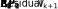
\includegraphics[keepaspectratio]{lec1-vecspace_files/figure-pdf/fig-venn-nested-projection-1.pdf}}

}

\caption{\label{fig-venn-nested-projection}Venn Diagram of Nested
Projections with Colored Increments}

\end{figure}%

\bookmarksetup{startatroot}

\chapter{Matrix Algebra}\label{matrix-algebra}

This chapter covers a review of matrix algebra concepts essential for
linear models, including eigenvalues, spectral decomposition, singular
value decomposition.

\section{Eigenvalues and
Eigenvectors}\label{eigenvalues-and-eigenvectors}

\begin{definition}[Eigenvalues and
Eigenvectors]\protect\hypertarget{def-eigen}{}\label{def-eigen}

For a square matrix \(A\) (\(n \times n\)), a scalar \(\lambda\) is an
\textbf{eigenvalue} and a non-zero vector \(x\) is the corresponding
\textbf{eigenvector} if:

\[
Ax = \lambda x \iff (A - \lambda I_n)x = 0
\]

The eigenvalues are found by solving the characteristic equation: \[
|A - \lambda I_n| = 0
\]

\end{definition}

\section{Spectral Theory for Symmetric
Matrices}\label{spectral-theory-for-symmetric-matrices}

\subsection{Spectral Decomposition}\label{spectral-decomposition}

For symmetric matrices, we have a powerful decomposition theorem.

\begin{theorem}[Spectral
Decomposition]\protect\hypertarget{thm-spectral}{}\label{thm-spectral}

If \(A\) is a symmetric \(n \times n\) matrix, all its eigenvalues
\(\lambda_1, \dots, \lambda_n\) are real. Furthermore, there exists an
orthogonal matrix \(Q\) such that:

\[
A = Q \Lambda Q' = \sum_{i=1}^n \lambda_i q_i q_i'
\]

where:

\begin{itemize}
\tightlist
\item
  \(\Lambda = \text{diag}(\lambda_1, \dots, \lambda_n)\) contains the
  eigenvalues.
\item
  \(Q = (q_1, \dots, q_n)\) contains the corresponding orthonormal
  eigenvectors (\(q_i'q_j = \delta_{ij}\)).
\end{itemize}

\end{theorem}

\textbf{Explantion}: This allows us to view the transformation \(Ax\) as
a rotation (\(Q'\)), a scaling (\(\Lambda\)), and a rotation back
(\(Q\)). For a symmetric matrix \(A\), we can write the spectral
decomposition as a product of the eigenvector matrix \(Q\) and
eigenvalue matrix \(\Lambda\):

\[
\begin{aligned}
A &= Q \Lambda Q' \\
  &= \begin{pmatrix} q_1 & q_2 & \cdots & q_n \end{pmatrix} 
     \begin{pmatrix} \lambda_1 & 0 & \cdots & 0 \\ 0 & \lambda_2 & \cdots & 0 \\ \vdots & \vdots & \ddots & \vdots \\ 0 & 0 & \cdots & \lambda_n \end{pmatrix} 
     \begin{pmatrix} q_1' \\ q_2' \\ \vdots \\ q_n' \end{pmatrix} \\
  &= \begin{pmatrix} \lambda_1 q_1 & \lambda_2 q_2 & \cdots & \lambda_n q_n \end{pmatrix} 
     \begin{pmatrix} q_1' \\ q_2' \\ \vdots \\ q_n' \end{pmatrix} \\
  &= \lambda_1 q_1 q_1' + \lambda_2 q_2 q_2' + \cdots + \lambda_n q_n q_n' \\
  &= \sum_{i=1}^n \lambda_i q_i q_i'
\end{aligned}
\]

where the eigenvectors \(q_i\) satisfy the orthogonality conditions: \[
q_i' q_j = \begin{cases} 1 & \text{if } i=j \\ 0 & \text{if } i \ne j \end{cases}
\] And \(Q\) is an orthogonal matrix: \(Q'Q = Q Q' = I_n\).

\begin{figure}

\centering{

\pandocbounded{\includegraphics[keepaspectratio]{lec2-matrix_files/figure-pdf/fig-eigen-1.pdf}}

}

\caption{\label{fig-eigen}}

\end{figure}%

\subsection{Quadratic Form}\label{quadratic-form}

\begin{definition}[]\protect\hypertarget{def-quadratic-form}{}\label{def-quadratic-form}

A \textbf{quadratic form} in \(n\) variables \(x_1, x_2, \dots, x_n\) is
a scalar function defined by a symmetric matrix \(A\): \[
Q(x) = x'Ax = \sum_{i=1}^n \sum_{j=1}^n a_{ij} x_i x_j
\]

\end{definition}

\subsection{Positive and Non-Negative Definite
Matrices}\label{positive-and-non-negative-definite-matrices}

\begin{definition}[Positive and Non-Negative Definite
Matrices]\protect\hypertarget{def-pos-def}{}\label{def-pos-def}

A symmetric matrix \(A\) is \textbf{positive definite (p.d.)} if: \[
x'Ax > 0 \quad \forall x \ne 0
\] It is \textbf{non-negative definite (n.n.d.)} if: \[
x'Ax \ge 0 \quad \forall x
\]

\end{definition}

\begin{theorem}[Properties of Definite
Matrices]\protect\hypertarget{thm-nnd-properties}{}\label{thm-nnd-properties}

Let \(A\) be a symmetric \(n \times n\) matrix with eigenvalues
\(\lambda_1, \dots, \lambda_n\).

\begin{enumerate}
\def\labelenumi{\arabic{enumi}.}
\item
  \textbf{Eigenvalue Characterization:}

  \begin{itemize}
  \tightlist
  \item
    \(A\) is p.d. \(\iff\) all \(\lambda_i > 0\).
  \item
    \(A\) is n.n.d. \(\iff\) all \(\lambda_i \ge 0\).
  \end{itemize}
\item
  \textbf{Determinant and Inverse:}

  \begin{itemize}
  \tightlist
  \item
    If \(A\) is p.d., then \(|A| > 0\) and \(A^{-1}\) exists.
  \item
    If \(A\) is n.n.d. and singular, then \(|A| = 0\) (at least one
    \(\lambda_i = 0\)).
  \end{itemize}
\item
  \textbf{Gram Matrices (\(B'B\)):} Let \(B\) be an \(n \times p\)
  matrix.

  \begin{itemize}
  \tightlist
  \item
    If \(\text{rank}(B) = p\), then \(B'B\) is p.d.
  \item
    If \(\text{rank}(B) < p\), then \(B'B\) is n.n.d.
  \end{itemize}
\end{enumerate}

\end{theorem}

\subsection{Properties of Symmetric
Matrices}\label{properties-of-symmetric-matrices}

\begin{theorem}[Properties of Symmetric
Matrices]\protect\hypertarget{thm-symmetric-properties}{}\label{thm-symmetric-properties}

Let \(A\) be a symmetric matrix with spectral decomposition
\(A = Q \Lambda Q'\). The following properties hold:

\begin{enumerate}
\def\labelenumi{\arabic{enumi}.}
\tightlist
\item
  \textbf{Trace:} \(\text{tr}(A) = \sum \lambda_i\).
\item
  \textbf{Determinant:} \(|A| = \prod \lambda_i\).
\item
  \textbf{Singularity:} \(A\) is singular if and only if at least one
  \(\lambda_i = 0\).
\item
  \textbf{Inverse:} If \(A\) is non-singular (\(\lambda_i \ne 0\)), then
  \(A^{-1} = Q \Lambda^{-1} Q'\).
\item
  \textbf{Powers:} \(A^k = Q \Lambda^k Q'\).

  \begin{itemize}
  \tightlist
  \item
    \emph{Square Root:} \(A^{1/2} = Q \Lambda^{1/2} Q'\) (if
    \(\lambda_i \ge 0\)).
  \end{itemize}
\item
  \textbf{Spectral Representation of Quadratic Forms:} The quadratic
  form \(x'Ax\) can be diagonalized using the eigenvectors of \(A\): \[
  x'Ax = x' Q \Lambda Q' x = y' \Lambda y = \sum_{i=1}^n \lambda_i y_i^2
  \] where \(y = Q'x\) represents a rotation of the coordinate system.
\end{enumerate}

\end{theorem}

\subsection{Spectral Representation of Projection
Matrices}\label{spectral-representation-of-projection-matrices}

We revisit projection matrices in the context of eigenvalues.

\begin{theorem}[Eigenvalues of Projection
Matrices]\protect\hypertarget{thm-proj-eigen}{}\label{thm-proj-eigen}

A symmetric matrix \(P\) is a projection matrix (idempotent, \(P^2=P\))
if and only if its eigenvalues are either 0 or 1.

\[
P^2 x = \lambda^2 x \quad \text{and} \quad Px = \lambda x \implies \lambda^2 = \lambda \implies \lambda \in \{0, 1\}
\]

\end{theorem}

For a projection matrix \(P\):

\begin{itemize}
\tightlist
\item
  If \(x \in \text{Col}(P)\), \(Px = x\) (Eigenvalue 1).
\item
  If \(x \perp \text{Col}(P)\), \(Px = 0\) (Eigenvalue 0).
\item
  \(\text{rank}(P) = \text{tr}(P) = \sum \lambda_i\) (Count of 1s).
\end{itemize}

\begin{example}[]\protect\hypertarget{exm-trace-P}{}\label{exm-trace-P}

For \(P = \frac{1}{n} J_n J_n'\), the rank is \(\text{tr}(P) = 1\).

\end{example}

\section{Singular Value Decomposition
(SVD)}\label{singular-value-decomposition-svd}

\begin{theorem}[Singular Value Decomposition
(SVD)]\protect\hypertarget{thm-svd}{}\label{thm-svd}

Let \(X\) be an \(n \times p\) matrix with rank \(r \le \min(n, p)\).
\(X\) can be decomposed into the product of three matrices:

\[
X = U \mathbf{D} V'
\]

\begin{enumerate}
\def\labelenumi{\arabic{enumi}.}
\tightlist
\item
  Partitioned Matrix Form
\end{enumerate}

\[
X = \underset{n \times n}{(U_1, U_2)}
\begin{pmatrix}
\Lambda_r & O_{r \times (p-r)} \\
O_{(n-r) \times r} & O_{(n-r) \times (p-r)}
\end{pmatrix}
\underset{p \times p}{
\begin{pmatrix}
V_1' \\
V_2'
\end{pmatrix}
}
\]

\begin{enumerate}
\def\labelenumi{\arabic{enumi}.}
\setcounter{enumi}{1}
\tightlist
\item
  Detailed Matrix Form
\end{enumerate}

Expanding the diagonal matrix explicitly:

\[
X = \underset{n \times n}{(u_1, \dots, u_n)}
\left(
\begin{array}{cccc|c}
\lambda_1 & 0 & \dots & 0 &  \\
0 & \lambda_2 & \dots & 0 & O_{12} \\
\vdots & \vdots & \ddots & \vdots &  \\
0 & 0 & \dots & \lambda_r &  \\
\hline
 & O_{21} & & & O_{22}
\end{array}
\right)
\underset{p \times p}{
\begin{pmatrix}
v_1' \\
\vdots \\
v_p'
\end{pmatrix}
}
\]

\begin{enumerate}
\def\labelenumi{\arabic{enumi}.}
\setcounter{enumi}{2}
\tightlist
\item
  Reduced Form
\end{enumerate}

\[
X = U_1 \Lambda_r V_1' = \sum_{i=1}^r \lambda_i u_i v_i'
\]

\textbf{Properties:}

\begin{enumerate}
\def\labelenumi{\arabic{enumi}.}
\tightlist
\item
  \textbf{Singular Values (\(\Lambda_r\)):}
  \(\Lambda_r = \text{diag}(\lambda_1, \dots, \lambda_r)\) contains the
  singular values (\(\lambda_i > 0\)), which are the square roots of the
  non-zero eigenvalues of \(X'X\).
\item
  \textbf{Orthogonality:}

  \begin{itemize}
  \tightlist
  \item
    \(U\) is \(n \times n\) orthogonal (\(U'U = I_n\)).
  \item
    \(V\) is \(p \times p\) orthogonal (\(V'V = I_p\)).
  \end{itemize}
\end{enumerate}

\end{theorem}

\subsubsection{Connection to Gram
Matrices}\label{connection-to-gram-matrices}

The matrices \(U\) and \(V\) provide the basis vectors (eigenvectors)
for the Gram matrices of \(X\).

\begin{enumerate}
\def\labelenumi{\arabic{enumi}.}
\item
  \textbf{Right Singular Vectors (\(V\)):} The columns of \(V\) are the
  eigenvectors of the Gram matrix \(X'X\). \[
  X'X = (U \Lambda V')' (U \Lambda V') = V \Lambda U' U \Lambda V' = V \Lambda^2 V'
  \]

  \begin{itemize}
  \tightlist
  \item
    The eigenvalues of \(X'X\) are the squared singular values
    \(\lambda_i^2\).
  \end{itemize}
\item
  \textbf{Left Singular Vectors (\(U\)):} The columns of \(U\) are the
  eigenvectors of the Gram matrix \(XX'\). \[
  XX' = (U \Lambda V') (U \Lambda V')' = U \Lambda V' V \Lambda U' = U \Lambda^2 U'
  \]

  \begin{itemize}
  \tightlist
  \item
    The eigenvalues of \(XX'\) are also \(\lambda_i^2\) (for non-zero
    values).
  \end{itemize}
\end{enumerate}

\begin{example}[Example of
SVD]\protect\hypertarget{exm-svd}{}\label{exm-svd}

Consider the matrix
\(X = \begin{pmatrix} 1 & 1 \\ 2 & 2 \end{pmatrix}\).

\begin{enumerate}
\def\labelenumi{\arabic{enumi}.}
\item
  \textbf{Compute \(X'X\) and find \(V\):} \[
  X'X = \begin{pmatrix} 1 & 2 \\ 1 & 2 \end{pmatrix} \begin{pmatrix} 1 & 1 \\ 2 & 2 \end{pmatrix} = \begin{pmatrix} 5 & 5 \\ 5 & 5 \end{pmatrix}
  \]

  \begin{itemize}
  \tightlist
  \item
    Eigenvalues of \(X'X\): Trace is 10, Determinant is 0. Thus,
    \(\mu_1 = 10, \mu_2 = 0\).
  \item
    \textbf{Singular Values:} \(\lambda_1 = \sqrt{10}, \lambda_2 = 0\).
  \item
    Eigenvector for \(\mu_1=10\): Normalized
    \(v_1 = \frac{1}{\sqrt{2}}\begin{pmatrix} 1 \\ 1 \end{pmatrix}\).
  \item
    Eigenvector for \(\mu_2=0\): Normalized
    \(v_2 = \frac{1}{\sqrt{2}}\begin{pmatrix} 1 \\ -1 \end{pmatrix}\).
  \item
    Therefore,
    \(V = \frac{1}{\sqrt{2}}\begin{pmatrix} 1 & 1 \\ 1 & -1 \end{pmatrix}\).
  \end{itemize}
\item
  \textbf{Compute \(XX'\) and find \(U\):} \[
  XX' = \begin{pmatrix} 1 & 1 \\ 2 & 2 \end{pmatrix} \begin{pmatrix} 1 & 2 \\ 1 & 2 \end{pmatrix} = \begin{pmatrix} 2 & 4 \\ 4 & 8 \end{pmatrix}
  \]

  \begin{itemize}
  \tightlist
  \item
    Eigenvalues are again 10 and 0.
  \item
    Eigenvector for \(\mu_1=10\): Normalized
    \(u_1 = \frac{1}{\sqrt{5}}\begin{pmatrix} 1 \\ 2 \end{pmatrix}\).
  \item
    Eigenvector for \(\mu_2=0\): Normalized
    \(u_2 = \frac{1}{\sqrt{5}}\begin{pmatrix} 2 \\ -1 \end{pmatrix}\).
  \item
    Therefore,
    \(U = \frac{1}{\sqrt{5}}\begin{pmatrix} 1 & 2 \\ 2 & -1 \end{pmatrix}\).
  \end{itemize}
\item
  \textbf{Verification:} \[
  X = \sqrt{10} u_1 v_1' = \sqrt{10} \begin{pmatrix} \frac{1}{\sqrt{5}} \\ \frac{2}{\sqrt{5}} \end{pmatrix} \begin{pmatrix} \frac{1}{\sqrt{2}} & \frac{1}{\sqrt{2}} \end{pmatrix} = \begin{pmatrix} 1 & 1 \\ 2 & 2 \end{pmatrix}
  \]
\end{enumerate}

\end{example}

\section{Cholesky Decomposition}\label{cholesky-decomposition}

A symmetric matrix \(A\) has a Cholesky decomposition if and only if it
is \textbf{non-negative definite} (i.e., \(x'Ax \ge 0\) for all \(x\)).

\[
A = B'B
\]

where \(B\) is an \textbf{upper triangular} matrix with non-negative
diagonal entries.

\subsection{Matrix Representation of the
Algorithm}\label{matrix-representation-of-the-algorithm}

To derive the algorithm, we equate the elements of \(A\) with the
product of the lower triangular matrix \(B'\) and the upper triangular
matrix \(B\).

For a \(3 \times 3\) matrix, this looks like:

\[
\underbrace{\begin{pmatrix}
a_{11} & a_{12} & a_{13} \\
a_{21} & a_{22} & a_{23} \\
a_{31} & a_{32} & a_{33}
\end{pmatrix}}_{A}
=
\underbrace{\begin{pmatrix}
b_{11} & 0 & 0 \\
b_{12} & b_{22} & 0 \\
b_{13} & b_{23} & b_{33}
\end{pmatrix}}_{B'}
\underbrace{\begin{pmatrix}
b_{11} & b_{12} & b_{13} \\
0 & b_{22} & b_{23} \\
0 & 0 & b_{33}
\end{pmatrix}}_{B}
\]

Multiplying the matrices on the right yields the system of equations:

\[
A = \begin{pmatrix}
\mathbf{b_{11}^2} & b_{11}b_{12} & b_{11}b_{13} \\
b_{12}b_{11} & \mathbf{b_{12}^2 + b_{22}^2} & b_{12}b_{13} + b_{22}b_{23} \\
b_{13}b_{11} & b_{13}b_{12} + b_{23}b_{22} & \mathbf{b_{13}^2 + b_{23}^2 + b_{33}^2}
\end{pmatrix}
\]

By solving for the bolded diagonal terms and substituting known values
from previous rows, we get the recursive algorithm.

\begin{algorithm}[Choleski
Decomposition]\protect\hypertarget{alg-chosk-decomp}{}\label{alg-chosk-decomp}

~

\begin{enumerate}
\def\labelenumi{\arabic{enumi}.}
\tightlist
\item
  \textbf{Row 1:} Solve for \(b_{11}\) using \(a_{11}\), then solve the
  rest of the row (\(b_{1j}\)) by division.

  \begin{itemize}
  \tightlist
  \item
    \(b_{11} = \sqrt{a_{11}}\)
  \item
    \(b_{1j} = a_{1j}/b_{11}\)
  \end{itemize}
\item
  \textbf{Row 2:} Solve for \(b_{22}\) using \(a_{22}\) and the known
  \(b_{12}\), then solve \(b_{2j}\).

  \begin{itemize}
  \tightlist
  \item
    \(b_{22} = \sqrt{a_{22} - b_{12}^2}\)
  \item
    \(b_{2j} = (a_{2j} - b_{12}b_{1j}) / b_{22}\)
  \end{itemize}
\item
  \textbf{Row 3:} Solve for \(b_{33}\) using \(a_{33}\) and the known
  \(b_{13}, b_{23}\).

  \begin{itemize}
  \tightlist
  \item
    \(b_{33} = \sqrt{a_{33} - b_{13}^2 - b_{23}^2}\)
  \end{itemize}
\end{enumerate}

\end{algorithm}

\begin{remark}
\textbf{Handling the Singular Case}

If \(A\) is positive semi-definite (singular), a diagonal element
\(b_{ii}\) may evaluate to 0 (or a very small number close to 0 due to
floating-point error). Standard algorithms often crash here because
calculating off-diagonal terms involves division by \(b_{ii}\).

To handle this robustly without pivoting:

\begin{itemize}
\tightlist
\item
  If \(b_{ii} \approx 0\), it implies that the entire remaining row
  \(b_{i, i:n}\) must be 0 for the matrix to remain consistent with
  being positive semi-definite.
\item
  The algorithm should explicitly set \(b_{ij} = 0\) for all \(j \ge i\)
  and proceed to the next row, rather than attempting division.
\end{itemize}

\end{remark}

\begin{example}[Example of Cholesky
Decomposition]\protect\hypertarget{exm-chol}{}\label{exm-chol}

Consider the positive definite matrix \(A\): \[
A = \begin{pmatrix}
4 & 2 & -2 \\
2 & 10 & 2 \\
-2 & 2 & 6
\end{pmatrix}
\]

We find \(B\) such that \(A = B'B\):

\begin{enumerate}
\def\labelenumi{\arabic{enumi}.}
\tightlist
\item
  \textbf{First Row of B (\(b_{11}, b_{12}, b_{13}\)):}

  \begin{itemize}
  \tightlist
  \item
    \(b_{11} = \sqrt{4} = 2\)
  \item
    \(b_{12} = 2 / 2 = 1\)
  \item
    \(b_{13} = -2 / 2 = -1\)
  \end{itemize}
\item
  \textbf{Second Row of B (\(b_{22}, b_{23}\)):}

  \begin{itemize}
  \tightlist
  \item
    \(b_{22} = \sqrt{10 - (1)^2} = \sqrt{9} = 3\)
  \item
    \(b_{23} = (2 - (1)(-1)) / 3 = 3/3 = 1\)
  \end{itemize}
\item
  \textbf{Third Row of B (\(b_{33}\)):}

  \begin{itemize}
  \tightlist
  \item
    \(b_{33} = \sqrt{6 - (-1)^2 - (1)^2} = \sqrt{4} = 2\)
  \end{itemize}
\end{enumerate}

\textbf{Result:} \[
B = \begin{pmatrix}
2 & 1 & -1 \\
0 & 3 & 1 \\
0 & 0 & 2
\end{pmatrix}
\]

\end{example}

\subsection{Applications in
Statistics}\label{applications-in-statistics}

Cholesky decomposition is preferred over other methods (like LU or SVD)
for symmetric positive-definite matrices because it is numerically
stable and roughly twice as fast.

\begin{enumerate}
\def\labelenumi{\arabic{enumi}.}
\item
  Solving Linear Equations

  In linear regression, we solve the normal equations
  \((X'X)\beta = X'y\). Since \(X'X\) is symmetric and positive
  definite, we can decompose it as \(B'B\). The system becomes: \[
   B'B\beta = X'y
   \] This allows us to solve for \(\beta\) using two efficient
  triangular substitutions (first solving \(B'z = X'y\) for \(z\), then
  \(B\beta = z\) for \(\beta\)) without explicitly inverting the matrix,
  which is computationally expensive and unstable.
\item
  Computing the Determinant

  The determinant of a triangular matrix is simply the product of its
  diagonal entries. Therefore, the determinant of \(A\) can be computed
  instantly from \(B\): \[
   \det(A) = \det(B'B) = \det(B')\det(B) = \left(\prod_{i=1}^n b_{ii}\right)^2
   \] This is widely used in Maximum Likelihood Estimation (e.g., REML
  in mixed models) where log-determinants of large covariance matrices
  are required.
\item
  Generating Multivariate Normal Random Variables

  To generate a random vector \(Y \sim N(\mu, \Sigma)\), we first
  generate a vector of independent standard normal variables
  \(Z \sim N(0, I)\). Using the Cholesky decomposition \(\Sigma = B'B\):
  \[
   Y = \mu + B'Z
   \] The covariance of \(Y\) is confirmed by
  \(\text{Cov}(Y) = B' \text{Cov}(Z) B = B' I B = B'B = \Sigma\). This
  is the standard method used by functions like \texttt{mvrnorm} in R.
\end{enumerate}

\bookmarksetup{startatroot}

\chapter{Multivariate Normal
Distribution}\label{multivariate-normal-distribution}

\section{Motivation}\label{motivation}

Consider the linear model: \[
y = X\beta + \epsilon, \quad \epsilon_i \sim N(0, \sigma^2)
\]

We are often interested in the distributional properties of the response
vector \(y\) and the residuals. Specifically, if
\(y = (y_1, \dots, y_n)'\), we need to understand its multivariate
distribution. \[
\hat{y} = Py, \quad e = y - \hat{y} = (I_n - P)y
\]

\section{Random Vectors and Matrices}\label{random-vectors-and-matrices}

\begin{definition}[Random Vector and
Matrix]\protect\hypertarget{def-random-vector}{}\label{def-random-vector}

A \textbf{Random Vector} is a vector whose elements are random
variables. E.g., \[
x_{k \times 1} = (x_1, x_2, \dots, x_k)^T
\] where \(x_1, \dots, x_k\) are each random variables.

A \textbf{Random Matrix} is a matrix whose elements are random
variables. E.g., \(X_{n \times k} = (x_{ij})\), where
\(x_{11}, \dots, x_{nk}\) are each random variables.

\end{definition}

\begin{definition}[Expected
Value]\protect\hypertarget{def-expected-value}{}\label{def-expected-value}

The expected value (population mean) of a random matrix (or vector) is
the matrix (or vector) of expected values of its elements.

For \(X_{n \times k}\): \[
E(X) = \begin{pmatrix}
E(x_{11}) & \dots & E(x_{1k}) \\
\vdots & \ddots & \vdots \\
E(x_{n1}) & \dots & E(x_{nk})
\end{pmatrix}
\]

\[
E\left(\begin{pmatrix} x_1 \\ \vdots \\ x_k \end{pmatrix}\right) = \begin{pmatrix} E(x_1) \\ \vdots \\ E(x_k) \end{pmatrix}
\]

\end{definition}

\begin{definition}[Variance-Covariance
Matrix]\protect\hypertarget{def-variance-covariance}{}\label{def-variance-covariance}

For a random vector \(x_{k \times 1} = (x_1, \dots, x_k)^T\), the matrix
is:

\[
\text{Var}(x) = \Sigma_x = \begin{pmatrix}
\sigma_{11} & \sigma_{12} & \dots & \sigma_{1k} \\
\sigma_{21} & \sigma_{22} & \dots & \sigma_{2k} \\
\vdots & \vdots & \ddots & \vdots \\
\sigma_{k1} & \sigma_{k2} & \dots & \sigma_{kk}
\end{pmatrix}
\]

Where:

\begin{itemize}
\tightlist
\item
  \(\sigma_{ij} = \text{Cov}(x_i, x_j) = E[(x_i - \mu_i)(x_j - \mu_j)]\)
\item
  \(\sigma_{ii} = \text{Var}(x_i) = E[(x_i - \mu_i)^2]\)
\end{itemize}

In matrix notation: \[
\text{Var}(x) = E[(x - \mu_x)(x - \mu_x)^T]
\] Note: \(\text{Var}(x)\) is symmetric.

\end{definition}

\subsection{Derivation of Covariance Matrix
Structure}\label{derivation-of-covariance-matrix-structure}

Expanding the vector multiplication for variance: \[
(x - \mu_x)(x - \mu_x)' \quad \text{where } \mu_x = (\mu_1, \dots, \mu_n)'
\] \[
= \begin{pmatrix} x_1 - \mu_1 \\ \vdots \\ x_n - \mu_n \end{pmatrix} (x_1 - \mu_1, \dots, x_n - \mu_n)
\] This results in the matrix \(A = (a_{ij})\) where
\(a_{ij} = (x_i - \mu_i)(x_j - \mu_j)\). Taking expectations yields the
covariance matrix elements \(\sigma_{ij}\).

\begin{definition}[Covariance Matrix (Two
Vectors)]\protect\hypertarget{def-covariance-matrix-two}{}\label{def-covariance-matrix-two}

For random vectors \(x_{k \times 1}\) and \(y_{n \times 1}\), the
covariance matrix is: \[
\text{Cov}(x, y) = E[(x - \mu_x)(y - \mu_y)^T] = \begin{pmatrix}
\text{Cov}(x_1, y_1) & \dots & \text{Cov}(x_1, y_n) \\
\vdots & \ddots & \vdots \\
\text{Cov}(x_k, y_1) & \dots & \text{Cov}(x_k, y_n)
\end{pmatrix}
\] Note that \(\text{Cov}(x, x) = \text{Var}(x)\).

\end{definition}

\begin{definition}[Correlation
Matrix]\protect\hypertarget{def-correlation-matrix}{}\label{def-correlation-matrix}

The correlation matrix of a random vector \(x\) is: \[
\text{corr}(x) = \begin{pmatrix}
1 & \rho_{12} & \dots & \rho_{1k} \\
\vdots & \ddots & \vdots \\
\rho_{k1} & \rho_{k2} & \dots & 1
\end{pmatrix}
\] where \(\rho_{ij} = \text{corr}(x_i, x_j)\).

\textbf{Relationships:} Let
\(V_x = \text{diag}(\text{Var}(x_1), \dots, \text{Var}(x_k))\). \[
\Sigma_x = V_x^{1/2} \rho_x V_x^{1/2} \quad \text{and} \quad \rho_x = (V_x^{1/2})^{-1} \Sigma_x (V_x^{1/2})^{-1}
\] Similarly for two vectors: \[
\Sigma_{xy} = V_x^{1/2} \rho_{xy} V_y^{1/2}
\]

\end{definition}

\section{Properties of Mean and
Variance}\label{properties-of-mean-and-variance}

We can derive several key algebraic properties for operations on random
vectors.

\begin{enumerate}
\def\labelenumi{\arabic{enumi}.}
\tightlist
\item
  \(E(X + Y) = E(X) + E(Y)\)
\item
  \(E(AXB) = A E(X) B\) (In particular, \(E(AX) = A\mu_x\))
\item
  \(\text{Cov}(x, y) = \text{Cov}(y, x)^T\)
\item
  \(\text{Cov}(x + c, y + d) = \text{Cov}(x, y)\)
\item
  \(\text{Cov}(Ax, By) = A \text{Cov}(x, y) B^T\)

  \begin{itemize}
  \tightlist
  \item
    Special case for scalars:
    \(\text{Cov}(ax, by) = ab \cdot \text{Cov}(x, y)\)
  \end{itemize}
\item
  \(\text{Cov}(x_1 + x_2, y_1) = \text{Cov}(x_1, y_1) + \text{Cov}(x_2, y_1)\)
\item
  \(\text{Var}(x + c) = \text{Var}(x)\)
\item
  \(\text{Var}(Ax) = A \text{Var}(x) A^T\)
\item
  \(\text{Var}(x_1 + x_2) = \text{Var}(x_1) + \text{Cov}(x_1, x_2) + \text{Cov}(x_2, x_1) + \text{Var}(x_2)\)
\item
  \(\text{Var}(\sum x_i) = \sum \text{Var}(x_i)\) if independent.
\end{enumerate}

\begin{proof}
\textbf{Property 5 (Covariance of Linear Transformation):} \[
\begin{aligned}
\text{Cov}(Ax, By) &= E[(Ax - A\mu_x)(By - B\mu_y)^T] \\
&= A E[(x - \mu_x)(y - \mu_y)^T] B^T \\
&= A \text{Cov}(x, y) B^T
\end{aligned}
\] \textbf{Property 2 (Expectation of Linear Transformation)}:

To prove \(E(AXB) = A E(X) B\): First consider \(E(Ax_j)\) where \(x_j\)
is a column of \(X\). \[
E(Ax_j) = E\begin{pmatrix} a_1' x_j \\ \vdots \\ a_n' x_j \end{pmatrix} = \begin{pmatrix} E(a_1' x_j) \\ \vdots \\ E(a_n' x_j) \end{pmatrix}
\] Since \(a_i\) are constants: \[
E(a_i' x_j) = E\left(\sum_{k=1}^p a_{ik} x_{kj}\right) = \sum_{k=1}^p a_{ik} E(x_{kj}) = a_i' E(x_j)
\] Thus \(E(Ax_j) = A E(x_j)\). Applying this to all columns of \(X\):
\[
E(AX) = [E(Ax_1), \dots, E(Ax_m)] = [AE(x_1), \dots, AE(x_m)] = A E(X)
\] Similarly, \(E(XB) = E(X)B\).

\textbf{Proof of Property 9 (Variance of Sum):}

\[
\text{Var}(x_1 + x_2) = E[(x_1 + x_2 - \mu_1 - \mu_2)(x_1 + x_2 - \mu_1 - \mu_2)^T]
\] Let centered variables be denoted by differences. \[
= E[((x_1 - \mu_1) + (x_2 - \mu_2))((x_1 - \mu_1) + (x_2 - \mu_2))^T]
\] Expanding terms: \[
= E[(x_1 - \mu_1)(x_1 - \mu_1)^T + (x_1 - \mu_1)(x_2 - \mu_2)^T + (x_2 - \mu_2)(x_1 - \mu_1)^T + (x_2 - \mu_2)(x_2 - \mu_2)^T]
\] \[
= \text{Var}(x_1) + \text{Cov}(x_1, x_2) + \text{Cov}(x_2, x_1) + \text{Var}(x_2)
\]
\end{proof}

\section{The Multivariate Normal
Distribution}\label{the-multivariate-normal-distribution}

\subsection{Definition and Density}\label{definition-and-density}

\begin{definition}[Independent Standard
Normal]\protect\hypertarget{def-standard-normal}{}\label{def-standard-normal}

Let \(z = (z_1, \dots, z_n)'\) where \(z_i \sim N(0, 1)\) are
independent. We say \(z \sim N_n(0, I_n)\). The joint PDF is the product
of marginals: \[
f(z) = \prod_{i=1}^n \frac{1}{\sqrt{2\pi}} e^{-\frac{z_i^2}{2}} = \frac{1}{(2\pi)^{n/2}} e^{-\frac{1}{2} z^T z}
\] Properties: \(E(z) = 0\) and \(\text{Var}(z) = I_n\) (Covariance is 0
for \(i \ne j\), Variance is 1).

\end{definition}

\begin{definition}[Multivariate Normal
Distribution]\protect\hypertarget{def-mvn}{}\label{def-mvn}

A random vector \(x\) (\(n \times 1\)) has a \textbf{multivariate normal
distribution} if it has the same distribution as: \[
x = A_{n \times p} z_{p \times 1} + \mu_{n \times 1}
\] where \(z \sim N_p(0, I_p)\), \(A\) is a matrix of constants, and
\(\mu\) is a vector of constants. The moments are:

\begin{itemize}
\tightlist
\item
  \(E(x) = \mu\)
\item
  \(\text{Var}(x) = AA^T = \Sigma\)
\end{itemize}

\end{definition}

\subsection{Geometric Interpretation}\label{geometric-interpretation}

Using Spectral Decomposition, \(\Sigma = Q \Lambda Q'\). We can view the
transformation \(x = Az + \mu\) as:

\begin{enumerate}
\def\labelenumi{\arabic{enumi}.}
\tightlist
\item
  Scaling by eigenvalues (\(\Lambda^{1/2}\)).
\item
  Rotation by eigenvectors (\(Q\)).
\item
  Shift by mean (\(\mu\)).
\end{enumerate}

\subsection{Probability Density
Function}\label{probability-density-function}

If \(\Sigma\) is positive definite, the PDF exists. We use the change of
variable formula for \(x = Az + \mu\): \[
f_x(x) = f_z(g^{-1}(x)) \cdot |J|
\] where \(z = A^{-1}(x - \mu)\) and \(J = \det(A^{-1}) = |A|^{-1}\).

\[
f_x(x) = (2\pi)^{-p/2} |A|^{-1} \exp \left\{ -\frac{1}{2} (A^{-1}(x-\mu))^T (A^{-1}(x-\mu)) \right\}
\]

Using \(|\Sigma| = |AA^T| = |A|^2\) and \(\Sigma^{-1} = (AA^T)^{-1}\),
we get: \[
f_x(x) = (2\pi)^{-p/2} |\Sigma|^{-1/2} \exp \left\{ -\frac{1}{2} (x-\mu)^T \Sigma^{-1} (x-\mu) \right\}
\]

\subsection{Moment Generating
Function}\label{moment-generating-function}

\begin{definition}[Moment Generating Function
(MGF)]\protect\hypertarget{def-mgf}{}\label{def-mgf}

The MGF of a random vector \(x\) is \(M_x(t) = E(e^{t^T x})\). For
\(x = Az + \mu\): \[
M_x(t) = E[e^{t^T(Az + \mu)}] = e^{t^T\mu} E[e^{(A^T t)^T z}] = e^{t^T\mu} M_z(A^T t)
\] Since \(M_z(u) = e^{u^T u / 2}\): \[
M_x(t) = e^{t^T\mu} \exp\left( \frac{1}{2} t^T (AA^T) t \right) = \exp \left( t^T\mu + \frac{1}{2} t^T \Sigma t \right)
\]

\end{definition}

Key Properties:

\begin{enumerate}
\def\labelenumi{\arabic{enumi}.}
\item
  \textbf{Uniqueness:} Two random vectors with the same MGF have the
  same distribution.
\item
  \textbf{Independence:} \(y_1\) and \(y_2\) are independent iff
  \(M_y(t) = M_{y_1}(t_1) M_{y_2}(t_2)\).
\end{enumerate}

\section{Construction and Linear
Transformations}\label{construction-and-linear-transformations}

\begin{theorem}[Constructing MVN Random
Vector]\protect\hypertarget{thm-construction}{}\label{thm-construction}

Let \(\mu \in \mathbb{R}^n\) and \(\Sigma\) be an \(n \times n\)
symmetric non-negative definitive (n.n.d) matrix. Then there exists a
multivariate normal distribution with mean \(\mu\) and covariance
\(\Sigma\).

\end{theorem}

\begin{proof}
Since \(\Sigma\) is n.n.d., there exists \(B\) such that
\(\Sigma = BB^T\) (e.g., via Cholesky or Spetral Decomposition). Let
\(z \sim N_n(0, I)\) and define \(x = Bz + \mu\).
\end{proof}

\begin{theorem}[Linear Transformation
Theorem]\protect\hypertarget{thm-linear-transform}{}\label{thm-linear-transform}

Let \(x \sim N_n(\mu, \Sigma)\). Let \(y = Cx + d\) where \(C\) is
\(r \times n\) and \(d\) is \(r \times 1\). Then: \[
y \sim N_r(C\mu + d, C \Sigma C^T)
\]

\end{theorem}

\begin{proof}
\(x = Az + \mu\) where \(AA^T = \Sigma\). \[
y = C(Az + \mu) + d = (CA)z + (C\mu + d)
\] This fits the definition of MVN with mean \(C\mu + d\) and variance
\(C \Sigma C^T\).
\end{proof}

\subsection{\texorpdfstring{Important Corollaries of
Theorem~\ref{thm-linear-transform}}{Important Corollaries of Theorem~}}\label{important-corollaries-of-thm-linear-transform}

\begin{corollary}[Marginals]\protect\hypertarget{cor-marginals}{}\label{cor-marginals}

Any subvector of a multivariate normal vector is also multivariate
normal.

\end{corollary}

\begin{proof}
If we partition \(x = (x_1', x_2')'\), we can use \(C = (I_r, 0)\) to
show \(x_1 \sim N(\mu_1, \Sigma_{11})\).
\end{proof}

\begin{corollary}[Univariate
Combinations]\protect\hypertarget{cor-univariate}{}\label{cor-univariate}

Any linear combination \(a^T x\) is univariate normal: \[
a^T x \sim N(a^T \mu, a^T \Sigma a)
\]

\end{corollary}

\begin{corollary}[Orthogonal
Transformations]\protect\hypertarget{cor-orthogonal}{}\label{cor-orthogonal}

If \(x \sim N(0, I_n)\) and \(Q\) is orthogonal (\(Q'Q = I\)), then
\(y = Q'x \sim N(0, I_n)\).

\end{corollary}

\begin{corollary}[Standardization]\protect\hypertarget{cor-standardization}{}\label{cor-standardization}

If \(y \sim N_n(\mu, \Sigma)\) and \(\Sigma\) is positive definite: \[
\Sigma^{-1/2}(y - \mu) \sim N_n(0, I_n)
\]

\end{corollary}

\begin{proof}
Let \(z = \Sigma^{-1/2}(y - \mu)\). Then
\(\text{Var}(z) = \Sigma^{-1/2} \Sigma \Sigma^{-1/2} = I_n\).
\end{proof}

\section{Independence}\label{independence}

\begin{theorem}[Independence in
MVN]\protect\hypertarget{thm-independence}{}\label{thm-independence}

Let \(y \sim N(\mu, \Sigma)\) be partitioned into \(y_1\) and \(y_2\).
\[
\Sigma = \begin{pmatrix} \Sigma_{11} & \Sigma_{12} \\ \Sigma_{21} & \Sigma_{22} \end{pmatrix}
\] Then \(y_1\) and \(y_2\) are independent if and only if
\(\Sigma_{12} = 0\) (zero covariance).

\end{theorem}

\begin{proof}
\leavevmode

\begin{enumerate}
\def\labelenumi{\arabic{enumi}.}
\item
  Independence \(\implies\) Covariance is 0: This holds generally for
  any distribution. \[
  \text{Cov}(y_1, y_2) = E[(y_1 - \mu_1)(y_2 - \mu_2)'] = 0
  \]
\item
  Covariance is 0 \(\implies\) Independence: This is specific to MVN. We
  use MGFs. If \(\Sigma_{12} = 0\), the quadratic form in the MGF
  splits: \[
  t^T \Sigma t = t_1^T \Sigma_{11} t_1 + t_2^T \Sigma_{22} t_2
  \] The MGF becomes: \[
  M_y(t) = \exp(t_1^T \mu_1 + \frac{1}{2} t_1^T \Sigma_{11} t_1) \times \exp(t_2^T \mu_2 + \frac{1}{2} t_2^T \Sigma_{22} t_2)
  \] \[
  M_y(t) = M_{y_1}(t_1) M_{y_2}(t_2)
  \] Thus, they are independent.
\end{enumerate}

\end{proof}

\section{Signal-Noise Decomposition for Multivariate Normal
Distribution}\label{signal-noise-decomposition-for-multivariate-normal-distribution}

We can formalize the relationship between two random vectors \(y\) and
\(x\) through a decomposition theorem that separates the systematic
signal from the stochastic noise.

\begin{theorem}[Regression Decomposition
Theorem]\protect\hypertarget{thm-reg-decomp}{}\label{thm-reg-decomp}

Let the random vector \(V\) of dimension \(p \times 1\) be partitioned
into two subvectors \(y\) (\(p_1 \times 1\)) and \(x\)
(\(p_2 \times 1\)). Assume \(V\) follows a multivariate normal
distribution:

\[
\begin{pmatrix} y \\ x \end{pmatrix} \sim N_p\left( \begin{pmatrix} \mu_y \\ \mu_x \end{pmatrix}, \begin{pmatrix} \Sigma_{yy} & \Sigma_{yx} \\ \Sigma_{xy} & \Sigma_{xx} \end{pmatrix} \right)
\]

The response vector \(y\) can be uniquely decomposed into a systematic
component and a stochastic error: \[
y = m(x) + e
\] where we define the \textbf{Regression Coefficient Matrix} \(B\) and
the components as:

\[
B = \Sigma_{yx}\Sigma_{xx}^{-1}
\]

\[
m(x) = \mu_y + B(x - \mu_x)
\]

\[
e = y - m(x)
\]

\textbf{Properties:}

\begin{enumerate}
\def\labelenumi{\arabic{enumi}.}
\item
  \textbf{Independence:} The noise vector \(e\) is statistically
  independent of the predictor \(x\) (and consequently independent of
  \(m(x)\)).
\item
  \textbf{Marginal Distributions:}

  \begin{itemize}
  \tightlist
  \item
    \(m(x) \sim N_{p_1}(\mu_y, \; B \Sigma_{xx} B^T)\)
  \item
    \(e \sim N_{p_1}(0, \; \Sigma_{yy} - B \Sigma_{xx} B^T)\)
  \end{itemize}
\item
  \textbf{Conditional Distribution:} Since \(y = m(x) + e\), and \(e\)
  is independent of \(x\), the conditional distribution is: \[
  y | x \sim N_{p_1}(m(x), \Sigma_{y|x})
  \] where: \[
  m(x) = \mu_y + B(x - \mu_x) = \mu_y + \Sigma_{yx}\Sigma_{xx}^{-1}(x - \mu_x)
  \] \[
  \Sigma_{y|x} = \Sigma_{yy} - B \Sigma_{xx} B^T = \Sigma_{yy} - \Sigma_{yx}\Sigma_{xx}^{-1}\Sigma_{xy}
  \]
\end{enumerate}

\end{theorem}

\begin{proof}
We define a transformation from the input vector
\(V = \begin{pmatrix} y \\ x \end{pmatrix}\) to the target vector
\(W = \begin{pmatrix} m(x) \\ e \end{pmatrix}\).

Using the linear transformation \(W = CV + d\):

\[
\underbrace{\begin{pmatrix} m(x) \\ e \end{pmatrix}}_{W} = \underbrace{\begin{pmatrix} 0 & B \\ I & -B \end{pmatrix}}_{C} \underbrace{\begin{pmatrix} y \\ x \end{pmatrix}}_{V} + \underbrace{\begin{pmatrix} \mu_y - B \mu_x \\ -(\mu_y - B \mu_x) \end{pmatrix}}_{d}
\]

\begin{enumerate}
\def\labelenumi{\arabic{enumi}.}
\tightlist
\item
  Mean Vector
\end{enumerate}

\[
E[W] = C E[V] + d = \begin{pmatrix} 0 & B \\ I & -B \end{pmatrix} \begin{pmatrix} \mu_y \\ \mu_x \end{pmatrix} + \begin{pmatrix} \mu_y - B \mu_x \\ -\mu_y + B \mu_x \end{pmatrix} 
= \begin{pmatrix} B \mu_x \\ \mu_y - B \mu_x \end{pmatrix} + \begin{pmatrix} \mu_y - B \mu_x \\ -\mu_y + B \mu_x \end{pmatrix} 
= \begin{pmatrix} \mu_y \\ 0 \end{pmatrix}
\]

\begin{enumerate}
\def\labelenumi{\arabic{enumi}.}
\setcounter{enumi}{1}
\tightlist
\item
  Covariance Matrix
\end{enumerate}

We compute \(\text{Var}(W) = C \Sigma C^T\) directly:

\[
\begin{aligned}
C \Sigma C^T &= \begin{pmatrix} 0 & B \\ I & -B \end{pmatrix} \begin{pmatrix} \Sigma_{yy} & \Sigma_{yx} \\ \Sigma_{xy} & \Sigma_{xx} \end{pmatrix} \begin{pmatrix} 0 & I \\ B^T & -B^T \end{pmatrix} \\
&= \begin{pmatrix} B \Sigma_{xy} & B \Sigma_{xx} \\ \Sigma_{yy} - B \Sigma_{xy} & \Sigma_{yx} - B \Sigma_{xx} \end{pmatrix} \begin{pmatrix} 0 & I \\ B^T & -B^T \end{pmatrix} \\
&= \begin{pmatrix} B \Sigma_{xx} B^T & B \Sigma_{xy} - B \Sigma_{xx} B^T \\ \Sigma_{yx}B^T - B \Sigma_{xx} B^T & (\Sigma_{yy} - B \Sigma_{xy}) - (\Sigma_{yx} - B \Sigma_{xx})B^T \end{pmatrix} \\
&= \begin{pmatrix} B \Sigma_{xx} B^T & 0 \\ 0 & \Sigma_{yy} - B \Sigma_{xx} B^T \end{pmatrix}
\end{aligned}
\]

\begin{enumerate}
\def\labelenumi{\arabic{enumi}.}
\setcounter{enumi}{2}
\tightlist
\item
  Conditional Distribution
\end{enumerate}

We have established that \(y = m(x) + e\) where \(e\) is independent of
\(x\). To find the distribution of \(y\) conditional on \(x\), we
observe that \(m(x)\) becomes a constant vector when \(x\) is fixed, and
the randomness comes solely from \(e\):

\[
E[y|x] = m(x) + E[e|x] = m(x) + 0 = m(x)
\] \[
\text{Var}(y|x) = \text{Var}(m(x)|x) + \text{Var}(e|x) = 0 + \text{Var}(e) = \Sigma_{y|x}
\]

Thus, \(y | x \sim N(m(x), \Sigma_{y|x})\).
\end{proof}

\subsection{Connections with Other
Formulas}\label{connections-with-other-formulas}

\subsubsection{Rao-Blackwell Decomposition of
Variance}\label{rao-blackwell-decomposition-of-variance}

The Law of Total Variance (Rao-Blackwell theorem) allows us to decompose
the total variance of \(y\) into two orthogonal components based on the
predictor \(x\):

\[
\text{Var}(y) = \underbrace{E[\text{Var}(y | x)]}_{\text{Unexplained (Noise)}} + \underbrace{\text{Var}[E(y | x)]}_{\text{Explained (Signal)}}
\]

In the Multivariate Normal case, this decomposition perfectly aligns
with our regression model \(y = m(x) + e\).

\subsubsection*{Variance of Noise}\label{variance-of-noise}
\addcontentsline{toc}{subsubsection}{Variance of Noise}

This term represents the average variance remaining in \(y\) after
accounting for \(x\). It corresponds to the variance of the error term
\(e\):

\[
E[\text{Var}(y | x)] = \text{Var}(e) = \Sigma_{yy} - B \Sigma_{xx} B^T
\]

\subsubsection*{Variance of Signal}\label{variance-of-signal}
\addcontentsline{toc}{subsubsection}{Variance of Signal}

This term represents the variability of the conditional mean \(m(x)\)
itself. Using the matrix \(B\), this takes the quadratic form:

\[
\text{Var}[E(y | x)] = \text{Var}[m(x)] = B \Sigma_{xx} B^T
\]

\subsubsection*{Total Variance}\label{total-variance}
\addcontentsline{toc}{subsubsection}{Total Variance}

Summing the Signal and Noise components recovers the total marginal
variance of \(y\):

\[
\Sigma_{yy} = \underbrace{\Sigma_{yy} - B \Sigma_{xx} B^T}_{\text{Unexplained (Noise)}} + \underbrace{B \Sigma_{xx} B^T}_{\text{Explained (Signal)}}
\]

\subsubsection{Connection to OLS Regression
Estimators}\label{connection-to-ols-regression-estimators}

In OLS regression, centering the data allows us to separate the
intercept from the slopes. Let \(\mathbf{y}_c\) and \(\mathbf{X}_c\) be
the centered response and design matrices (where \(\mathbf{X}_c\)
\textbf{excludes the column of 1s}). Using this centered form, the total
sum of squares decomposes exactly like the population variance:

\[
\text{SST} = \text{SSR} + \text{SSE}
\]

Comparing the sample quantities to their population counterparts:

\begin{enumerate}
\def\labelenumi{\arabic{enumi}.}
\item
  \textbf{Regression Coefficients:} \[
    \hat{\beta}^T = (\mathbf{X}_c^T \mathbf{X}_c)^{-1} \mathbf{X}_c^T \mathbf{y}_c \approx B
    \] \emph{Note: \(\hat{\beta}\) here represents only the slope
  coefficients, matching the dimensions of the covariance matrix
  \(\Sigma_{xx}\).}
\item
  \textbf{Explained Variation (Signal):} \[
  \text{SSR} = \hat{\beta}^T (\mathbf{X}_c^T \mathbf{X}_c) \hat{\beta} \quad \approx \quad (n-1) B \Sigma_{xx} B^T
  \]
\item
  \textbf{Unexplained Variation (Noise):} \[
  \text{SSE} = \mathbf{y}_c^T \mathbf{y}_c - \hat{\beta}^T (\mathbf{X}_c^T \mathbf{X}_c) \hat{\beta} \quad \approx \quad (n-1)(\Sigma_{yy} - B \Sigma_{xx} B^T)
  \]
\end{enumerate}

\section{Partial and Multiple
Correlation}\label{partial-and-multiple-correlation}

\begin{definition}[Partial
Correlation]\protect\hypertarget{def-partial-corr}{}\label{def-partial-corr}

The partial correlation between elements \(y_i\) and \(y_j\) given a set
of variables \(x\) is derived from the conditional covariance matrix
\(\Sigma_{y|x}\): \[
\rho_{ij|x} = \frac{\sigma_{ij|x}}{\sqrt{\sigma_{ii|x} \sigma_{jj|x}}}
\] where \(\sigma_{ij|x}\) are elements of
\(\Sigma_{y|x} = \Sigma_{yy} - \Sigma_{yx}\Sigma_{xx}^{-1}\Sigma_{xy}\).

\end{definition}

\begin{definition}[Multiple Correlation
(\(R^2\))]\protect\hypertarget{def-multiple-corr}{}\label{def-multiple-corr}

For a scalar \(y\) and vector \(x\), the squared multiple correlation is
the proportion of variance of \(y\) explained by the conditional mean:
\[
R^2_{y|x} = \frac{\text{Var}(E(y|x))}{\text{Var}(y)} = \frac{\Sigma_{yx} \Sigma_{xx}^{-1} \Sigma_{xy}}{\sigma^2_{y}}
\]

\end{definition}

Note: this definition is the population or theretical \(R^2\), which is
estimated by adjusted \(R^2\) using sample in linear regression.

\section{Examples}\label{examples-1}

\begin{example}[Bivariate
Normal]\protect\hypertarget{exm-numerical}{}\label{exm-numerical}

Let the random vector \(\begin{pmatrix} y \\ x \end{pmatrix}\) follow a
bivariate normal distribution: \[
\begin{pmatrix} y \\ x \end{pmatrix} \sim N \left( \begin{pmatrix} 1 \\ 2 \end{pmatrix}, \begin{pmatrix} 2 & 2 \\ 2 & 4 \end{pmatrix} \right)
\] Here, \(\mu_y = 1, \mu_x = 2, \Sigma_{yy} = 2, \Sigma_{xx} = 4\), and
\(\Sigma_{yx} = 2\).

\begin{enumerate}
\def\labelenumi{\arabic{enumi}.}
\item
  Finding the Regression Coefficient Matrix \(B\) Using the population
  formula: \[
  B = \Sigma_{yx}\Sigma_{xx}^{-1} = 2(4)^{-1} = 0.5
  \]
\item
  Finding the Conditional Mean \(m(x)\) (The Signal) The systematic
  component represents the projection of \(y\) onto \(x\): \[
  \begin{aligned}
  m(x) &= \mu_y + B(x - \mu_x) \\
  &= 1 + 0.5(x - 2) = 0.5x
  \end{aligned}
  \]
\item
  Variance of the Signal \(\text{Var}(m(x))\) Using the quadratic form
  established in the theorem: \[
  \text{Var}(m(x)) = B \Sigma_{xx} B^T = 0.5(4)(0.5) = 1
  \]
\item
  Variance of the Noise \(\text{Var}(y|x)\) (The Residual) By the
  Signal-Noise Decomposition: \[
  \begin{aligned}
  \text{Var}(y|x) &= \Sigma_{yy} - \text{Var}(m(x)) \\
  &= 2 - 1 = 1
  \end{aligned}
  \] Thus, \(y | x \sim N(m(x), 1)\). The total variance (2) is split
  equally between signal (1) and noise (1).
\item
  Multiple Correlation Coefficient (\(R^2\)) \[
  R^2 = \frac{\text{Var}(m(x))}{\Sigma_{yy}} = \frac{1}{2} = 0.5
  \]
\end{enumerate}

\begin{figure}

\centering{

\pandocbounded{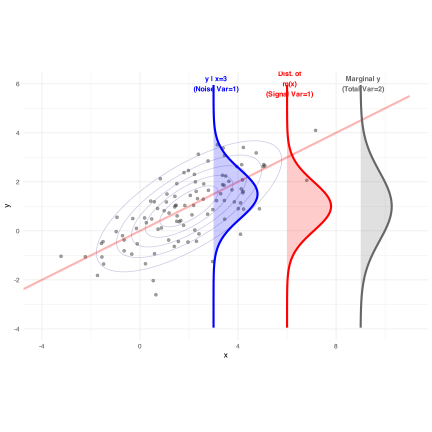
\includegraphics[keepaspectratio]{lec3-mvn_files/figure-pdf/fig-variance-decomp-scaled-1.pdf}}

}

\caption{\label{fig-variance-decomp-scaled}Illustration of Rao-Blackwell
Variance Decomposition in Bivariate Normal}

\end{figure}%

\end{example}

\begin{example}[Trivariate Normal with 2
Predictors]\protect\hypertarget{exm-trivariate}{}\label{exm-trivariate}

Let \(V = (y, x_1, x_2)' \sim N_3(\mu, \Sigma)\) with: \[
\mu = \begin{pmatrix} 1 \\ 2 \\ 3 \end{pmatrix}, \quad \Sigma = \begin{pmatrix} 10 & 3 & 4 \\ 3 & 2 & 1 \\ 4 & 1 & 4 \end{pmatrix}
\] We partition these into \(\Sigma_{yy} = 10\),
\(\Sigma_{yx} = \begin{pmatrix} 3 & 4 \end{pmatrix}\), and
\(\Sigma_{xx} = \begin{pmatrix} 2 & 1 \\ 1 & 4 \end{pmatrix}\).

\begin{enumerate}
\def\labelenumi{\arabic{enumi}.}
\item
  Finding the Regression Coefficient Matrix \(B\) \[
  \Sigma_{xx}^{-1} = \frac{1}{7} \begin{pmatrix} 4 & -1 \\ -1 & 2 \end{pmatrix} \implies B = \Sigma_{yx} \Sigma_{xx}^{-1} = \begin{pmatrix} \frac{8}{7} & \frac{5}{7} \end{pmatrix}
  \]
\item
  Finding the Conditional Mean \(m(x)\) (The Signal) \[
  m(x) = 1 + \frac{8}{7}(x_1 - 2) + \frac{5}{7}(x_2 - 3)
  \]
\item
  Variance of the Signal \(\text{Var}(m(x))\) \[
  \text{Var}(m(x)) = B \Sigma_{xx} B^T = \begin{pmatrix} \frac{8}{7} & \frac{5}{7} \end{pmatrix} \begin{pmatrix} 3 \\ 4 \end{pmatrix} = \frac{44}{7} \approx 6.29
  \]
\item
  Variance of the Noise \(\text{Var}(y|x)\) (The Residual) Using the
  Signal-Noise Decomposition: \[
  \Sigma_{y|x} = \Sigma_{yy} - \text{Var}(m(x)) = 10 - 6.29 = 3.71
  \]
\item
  Multiple Correlation Coefficient (\(R^2\)) \[
  R^2 = \frac{6.29}{10} = 0.629
  \]
\end{enumerate}

\begin{figure}

\centering{

\pandocbounded{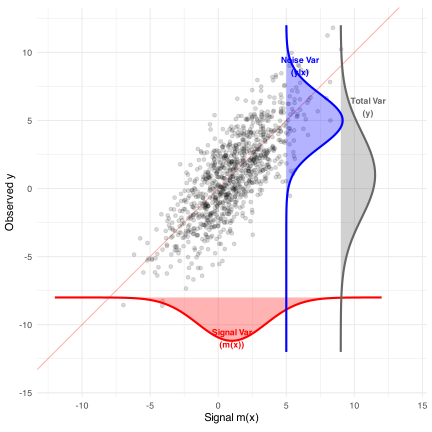
\includegraphics[keepaspectratio]{lec3-mvn_files/figure-pdf/fig-trivariate-refined-1.pdf}}

}

\caption{\label{fig-trivariate-refined}Signal-Noise Variance
Decomposition in Multivariate Normal}

\end{figure}%

\end{example}

\bookmarksetup{startatroot}

\chapter{Distribution of Quadratic
Forms}\label{distribution-of-quadratic-forms}

This chapter covers the distribution of quadratic forms (sums of
squares), which is crucial for hypothesis testing in linear models.

\section{Quadratic Forms}\label{quadratic-forms}

A quadratic form is a polynomial with terms all of degree two.

\begin{definition}[Quadratic
Form]\protect\hypertarget{def-quadratic-form}{}\label{def-quadratic-form}

Let \(y = (y_1, \dots, y_n)'\) be a random vector and \(A\) be a
symmetric \(n \times n\) matrix. The scalar quantity \(y'Ay\) is called
a \textbf{quadratic form} in \(y\).

\[
y'Ay = \sum_{i=1}^n \sum_{j=1}^n a_{ij} y_i y_j
\]

\end{definition}

\textbf{Examples:}

\begin{itemize}
\tightlist
\item
  \textbf{Squared Norm:} If \(A = I_n\), then
  \(y'I_n y = y'y = \sum y_i^2 = ||y||^2\).
\item
  \textbf{Weighted Sum of Squares:} If \(A\) is diagonal with elements
  \(\lambda_i\), then \(y'Ay = \sum \lambda_i y_i^2\).
\item
  \textbf{Projection Sum of Squares:} If \(P\) is a projection matrix,
  \(||Py||^2 = (Py)'(Py) = y'P'Py = y'Py\) (since \(P\) is symmetric and
  idempotent).
\end{itemize}

\section{Mean of Quadratic Forms}\label{mean-of-quadratic-forms}

We can find the expected value of a quadratic form without assuming
normality.

\begin{lemma}[Mean of Simplified Quadratic
Form]\protect\hypertarget{lem-simple-qf}{}\label{lem-simple-qf}

If \(y\) is a random vector with mean \(E(y) = \mu\) and covariance
matrix \(\text{Var}(y) = I_n\), then: \[
E(y'y) = \text{tr}(I_n) + \mu'\mu = n + \mu'\mu
\]

\end{lemma}

\begin{proof}
Let us decompose \(y\) into its mean and a stochastic component:
\(y = \mu + z\), where \(E(z) = 0\) and
\(\text{Var}(z) = E(zz') = I_n\). Substituting this into the quadratic
form: \[
\begin{aligned}
y'y &= (\mu + z)'(\mu + z) \\
&= \mu'\mu + \mu'z + z'\mu + z'z \\
&= \mu'\mu + 2\mu'z + z'z
\end{aligned}
\] Taking the expectation: \[
\begin{aligned}
E(y'y) &= \mu'\mu + 2\mu'E(z) + E(z'z) \\
&= \mu'\mu + 0 + E\left(\sum_{i=1}^n z_i^2\right)
\end{aligned}
\] Since \(\text{Var}(z_i) = E(z_i^2) - (E(z_i))^2 = 1 - 0 = 1\), we
have \(E(\sum z_i^2) = \sum 1 = n\). Thus, \(E(y'y) = n + \mu'\mu\).
\end{proof}

\begin{figure}

\centering{

\pandocbounded{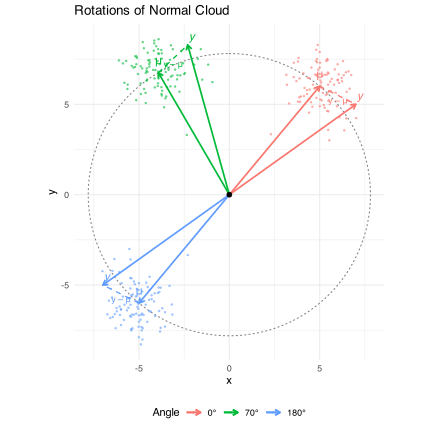
\includegraphics[keepaspectratio]{lec4-qf_files/figure-pdf/fig-qf-norm-1.pdf}}

}

\caption{\label{fig-qf-norm}Illustration of the Mean and Distribution of
Quadratic Forms}

\end{figure}%

\begin{theorem}[Mean of Quadratic
Form]\protect\hypertarget{thm-mean-qf}{}\label{thm-mean-qf}

If \(y\) is a random vector with mean \(E(y) = \mu\) and covariance
matrix \(\text{Var}(y) = \Sigma\), and \(A\) is a symmetric matrix of
constants, then:

\[
E(y'Ay) = \text{tr}(A\Sigma) + \mu'A\mu
\]

\end{theorem}

\begin{proof}
We present three methods to derive the expectation of the quadratic
form.

\textbf{Method 1: Using the Trace Trick}

Using the fact that a scalar is equal to its own trace
(\(\text{tr}(c) = c\)) and the linearity of expectation: \[
\begin{aligned}
E(y'Ay) &= E[\text{tr}(y'Ay)] \\
&= E[\text{tr}(Ayy')] \quad \text{(cyclic property of trace)} \\
&= \text{tr}(A E[yy']) \quad \text{(linearity of expectation)}
\end{aligned}
\] Recall that the covariance matrix is defined as
\(\Sigma = E[(y-\mu)(y-\mu)'] = E(yy') - \mu\mu'\). Rearranging this
gives the second moment: \(E(yy') = \Sigma + \mu\mu'\). Substituting
this back: \[
\begin{aligned}
E(y'Ay) &= \text{tr}(A(\Sigma + \mu\mu')) \\
&= \text{tr}(A\Sigma) + \text{tr}(A\mu\mu') \\
&= \text{tr}(A\Sigma) + \text{tr}(\mu'A\mu) \quad \text{(cyclic property on second term)} \\
&= \text{tr}(A\Sigma) + \mu'A\mu
\end{aligned}
\]

\textbf{Method 2: Using Scalar Summation}

We can express the quadratic form in scalar notation using the entries
of \(A=(a_{ij})\), \(\Sigma=(\sigma_{ij})\), and \(\mu=(\mu_i)\): \[
\begin{aligned}
E(y'Ay) &= E\left(\sum_{i=1}^n \sum_{j=1}^n a_{ij} y_i y_j\right) \\
&= \sum_{i=1}^n \sum_{j=1}^n a_{ij} E(y_i y_j) \\
&= \sum_{i=1}^n \sum_{j=1}^n a_{ij} (\sigma_{ij} + \mu_i \mu_j) \\
&= \sum_{i=1}^n \sum_{j=1}^n a_{ij} \sigma_{ji} + \sum_{i=1}^n \sum_{j=1}^n \mu_i a_{ij} \mu_j \quad (\text{since } \Sigma \text{ is symmetric, } \sigma_{ij}=\sigma_{ji}) \\
&= \text{tr}(A\Sigma) + \mu'A\mu
\end{aligned}
\]

\textbf{Method 3: Using Spectral Decomposition of A}

Since \(A\) is symmetric, we use its spectral decomposition
\(A = \sum_{i=1}^n \lambda_i q_i q_i'\). Substituting this into the
quadratic form: \[
y'Ay = y' \left( \sum_{i=1}^n \lambda_i q_i q_i' \right) y = \sum_{i=1}^n \lambda_i (q_i' y)^2
\] Let \(w_i = q_i' y\). This is a scalar random variable which is a
linear transformation of \(y\). Its properties are:

\begin{enumerate}
\def\labelenumi{\arabic{enumi}.}
\tightlist
\item
  \textbf{Mean:} \(E(w_i) = q_i' E(y) = q_i' \mu\).
\item
  \textbf{Variance:}
  \(\text{Var}(w_i) = \text{Var}(q_i' y) = q_i' \text{Var}(y) q_i = q_i' \Sigma q_i\).
\end{enumerate}

Using the relation \(E(w_i^2) = \text{Var}(w_i) + [E(w_i)]^2\), we have:
\[
E[(q_i' y)^2] = q_i' \Sigma q_i + (q_i' \mu)^2
\] Summing over all \(i\) weighted by \(\lambda_i\): \[
\begin{aligned}
E(y'Ay) &= \sum_{i=1}^n \lambda_i \left[ q_i' \Sigma q_i + (q_i' \mu)^2 \right] \\
&= \sum_{i=1}^n \text{tr}(\lambda_i q_i' \Sigma q_i) + \mu' \left( \sum_{i=1}^n \lambda_i q_i q_i' \right) \mu \\
&= \text{tr}\left( \Sigma \sum_{i=1}^n \lambda_i q_i q_i' \right) + \mu' A \mu \\
&= \text{tr}(\Sigma A) + \mu' A \mu
\end{aligned}
\]
\end{proof}

\begin{remark}[Geometric Interpretation via Sigma]
If we further decompose \(\Sigma = \sum_{j=1}^n \gamma_j v_j v_j'\)
(where \(\gamma_j, v_j\) are eigenvalues/vectors of \(\Sigma\)), the
trace term becomes: \[
\text{tr}(A\Sigma) = \sum_{i=1}^n \sum_{j=1}^n \lambda_i \gamma_j (q_i' v_j)^2
\] Here, \((q_i' v_j)^2 = \cos^2(\theta_{ij})\) represents the alignment
between the axes of the quadratic form (\(A\)) and the axes of the data
covariance (\(\Sigma\)). The expectation is maximized when the
eigenspaces of \(A\) and \(\Sigma\) align.
\end{remark}

\begin{corollary}[Expectation with Projection
Matrix]\protect\hypertarget{cor-projection-mean}{}\label{cor-projection-mean}

Consider the special case where:

\begin{enumerate}
\def\labelenumi{\arabic{enumi}.}
\tightlist
\item
  \(P\) is a \textbf{projection matrix} (symmetric and idempotent,
  \(P^2=P\)).
\item
  The covariance is \textbf{spherical}: \(\Sigma = \sigma^2 I_n\).
\end{enumerate}

Then the expectation simplifies to: \[
E(y'Py) = \sigma^2 r + ||P\mu||^2
\] where \(r = \text{rank}(P) = \text{tr}(P)\).

\textbf{Proof:} Using Theorem~\ref{thm-mean-qf} with \(A=P\) and
\(\Sigma=\sigma^2 I_n\):

\begin{enumerate}
\def\labelenumi{\arabic{enumi}.}
\tightlist
\item
  \textbf{Trace Term:}
  \(\text{tr}(P\Sigma) = \text{tr}(P(\sigma^2 I_n)) = \sigma^2 \text{tr}(P)\).
  Since \(P\) is idempotent, its eigenvalues are either 0 or 1, so
  \(\text{tr}(P) = \text{rank}(P) = r\).
\item
  \textbf{Mean Term:} Since \(P\) is symmetric and idempotent
  (\(P'P = P^2 = P\)), we can rewrite the quadratic form: \[
  \mu' P \mu = \mu' P' P \mu = (P\mu)' (P\mu) = ||P\mu||^2
  \]
\end{enumerate}

\end{corollary}

\begin{example}[Expectation of Sum of Squares Decomposition (i.i.d.
Case)]\protect\hypertarget{exm-mean-ss-decomposition}{}\label{exm-mean-ss-decomposition}

Consider a random vector \(y = (y_1, \dots, y_n)'\) with mean vector
\(\mu_y = \mu j_n\) and covariance \(\Sigma = \sigma^2 I_n\). We analyze
the two components of the total sum of squares by projecting \(y\) onto
the mean space (\(P_{j_n}\)) and the residual space (\(I-P_{j_n}\)).

\begin{enumerate}
\def\labelenumi{\arabic{enumi}.}
\tightlist
\item
  The Projection Vectors
\end{enumerate}

First, we write the explicit forms of the projected vectors using
\(P_{j_n} = \frac{1}{n}j_n j_n'\):

\begin{itemize}
\item
  \textbf{Mean Vector (\(P_{j_n}y\)):} Projecting \(y\) onto the column
  space of \(j_n\) replaces every element with the sample mean
  \(\bar{y}\). \[
    P_{j_n}y = \bar{y} j_n = \begin{pmatrix} \bar{y} \\ \bar{y} \\ \vdots \\ \bar{y} \end{pmatrix}
    \]
\item
  \textbf{Residual Vector (\((I-P_{j_n})y\)):} Subtracting the mean
  projection from \(y\) yields the deviations. \[
    (I-P_{j_n})y = y - \bar{y}j_n = \begin{pmatrix} y_1 - \bar{y} \\ y_2 - \bar{y} \\ \vdots \\ y_n - \bar{y} \end{pmatrix}
    \]
\end{itemize}

\begin{enumerate}
\def\labelenumi{\arabic{enumi}.}
\setcounter{enumi}{1}
\tightlist
\item
  Expectations of Squared Norms
\end{enumerate}

We now find the expectation of the squared length of these vectors using
Corollary~\ref{cor-projection-mean}.

\textbf{Part A: Sum of Squares for Mean} The quadratic form is the
squared norm of the projected mean vector: \[
y'P_{j_n}y = ||P_{j_n}y||^2 = \sum_{i=1}^n \bar{y}^2 = n\bar{y}^2
\] Applying the corollary with \(P=P_{j_n}\):

\begin{itemize}
\tightlist
\item
  \textbf{Rank:} \(\text{tr}(P_{j_n}) = 1\).
\item
  \textbf{Mean:} \(P_{j_n}\mu_y = P_{j_n}(\mu j_n) = \mu j_n\). The
  squared norm is \(n\mu^2\).
\end{itemize}

\[
E[||P_{j_n}y||^2] = \sigma^2(1) + n\mu^2
\]

\textbf{Part B: Sum of Squared Errors (SSE)} The quadratic form is the
squared norm of the residual vector: \[
y'(I-P_{j_n})y = ||(I-P_{j_n})y||^2 = \sum_{i=1}^n (y_i - \bar{y})^2
\] Applying the corollary with \(P=I-P_{j_n}\):

\begin{itemize}
\tightlist
\item
  \textbf{Rank:} \(\text{tr}(I-P_{j_n}) = n - 1\).
\item
  \textbf{Mean:}
  \((I-P_{j_n})\mu_y = \mu_y - P_{j_n}\mu_y = \mu j_n - \mu j_n = 0\).
  The squared norm is \(0\).
\end{itemize}

\[
E[||(I-P_{j_n})y||^2] = \sigma^2(n-1) + 0
\]

\textbf{Conclusion} These results confirm the standard properties:
\(E(\bar{y}^2) = \frac{\sigma^2}{n} + \mu^2\) and \(E(S^2) = \sigma^2\).

\end{example}

\begin{example}[Expectation of Total Sum of Squares (Regression
Case)]\protect\hypertarget{exm-mean-sst-regression}{}\label{exm-mean-sst-regression}

Consider now a regression setting where the mean of \(y\) depends on
covariates (e.g., \(\mu_i = \beta_0 + \beta_1 x_i\)). The mean vector
\(\mu_y\) is \textbf{not} proportional to \(j_n\). We are interested in
the expectation of the \textbf{Total Sum of Squares (SST)}.

\begin{enumerate}
\def\labelenumi{\arabic{enumi}.}
\item
  Identification The SST measures the variation of \(y\) around the
  \emph{global sample mean} \(\bar{y}\), ignoring the covariates: \[
  \text{SST} = \sum_{i=1}^n (y_i - \bar{y})^2 = y'(I - P_{j_n})y
  \] This is the same quadratic form as Part B in the previous example,
  but the underlying mean \(\mu_y\) has changed.
\item
  Calculation We apply Corollary~\ref{cor-projection-mean} with
  \(P = I - P_{j_n}\) and general \(\mu_y\):
\end{enumerate}

\begin{itemize}
\tightlist
\item
  \textbf{Rank Term:} Same as before,
  \(\text{tr}(I - P_{j_n}) = n - 1\).
\item
  \textbf{Mean Term:} The projection of the mean vector is no longer
  zero. \[
    (I - P_{j_n})\mu_y = \mu_y - \bar{\mu}j_n = \begin{pmatrix} \mu_1 - \bar{\mu} \\ \vdots \\ \mu_n - \bar{\mu} \end{pmatrix}
    \] where \(\bar{\mu} = \frac{1}{n}\sum \mu_i\) is the average of the
  true means. The squared norm is the sum of squared deviations of the
  true means: \[
    ||(I - P_{j_n})\mu_y||^2 = \sum_{i=1}^n (\mu_i - \bar{\mu})^2
    \]
\end{itemize}

\textbf{Conclusion} \[
E(\text{SST}) = (n-1)\sigma^2 + \sum_{i=1}^n (\mu_i - \bar{\mu})^2
\] This shows that in regression, the SST estimates \((n-1)\sigma^2\)
\emph{plus} the variability introduced by the regression signal (the
spread of the true means \(\mu_i\)).

\end{example}

\begin{figure}

\centering{

\pandocbounded{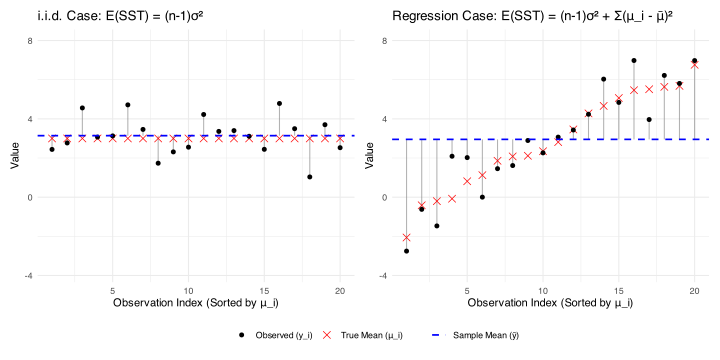
\includegraphics[keepaspectratio]{lec4-qf_files/figure-pdf/fig-sst-comparison-sorted-v2-1.pdf}}

}

\caption{\label{fig-sst-comparison-sorted-v2}Comparison of SST
components with increased variation in the true means. The vertical
lines represent the deviations \((y_i - \bar{y})\). With
\(\text{sd}(\mu_i) = 3\), the regression case (right) shows
significantly larger deviations, illustrating how the systematic spread
of the means dominates the Total Sum of Squares.}

\end{figure}%

\section{\texorpdfstring{Non-central \(\chi^2\)
Distribution}{Non-central \textbackslash chi\^{}2 Distribution}}\label{non-central-chi2-distribution}

To understand the distribution of quadratic forms under normality, we
introduce the non-central chi-square distribution.

\begin{definition}[Non-central \(\chi^2\)
Distribution]\protect\hypertarget{def-nc-chisq}{}\label{def-nc-chisq}

Let \(y \sim N_n(\mu, I_n)\). The random variable
\(V = y'y = \sum y_i^2\) follows a \textbf{non-central chi-square
distribution} with \(n\) degrees of freedom and non-centrality parameter
\(\lambda\).

\[
V \sim \chi^2(n, \lambda) \quad \text{where } \lambda = \mu'\mu = ||\mu||^2
\]

\end{definition}

\begin{tcolorbox}[enhanced jigsaw, toprule=.15mm, titlerule=0mm, left=2mm, bottomrule=.15mm, opacityback=0, colback=white, leftrule=.75mm, coltitle=black, colbacktitle=quarto-callout-important-color!10!white, colframe=quarto-callout-important-color-frame, arc=.35mm, rightrule=.15mm, breakable, bottomtitle=1mm, toptitle=1mm, title=\textcolor{quarto-callout-important-color}{\faExclamation}\hspace{0.5em}{Important}, opacitybacktitle=0.6]

\textbf{Note on NCP Definition:} Some definitions of non-central
\(\chi^2\) use \(\lambda = \frac{1}{2}\mu'\mu\). In this course, we use
\(\lambda = \mu'\mu\). With this convention, the Poisson-mixture
representation below uses Poisson(\(\lambda/2\)) weights.

\end{tcolorbox}

\subsection{\texorpdfstring{Visualizing \(\chi^2\)
Distributions}{Visualizing \textbackslash chi\^{}2 Distributions}}\label{visualizing-chi2-distributions}

Here is a plot visualizing the difference between central and
non-central Chi-square distributions.

\begin{figure}

\centering{

\pandocbounded{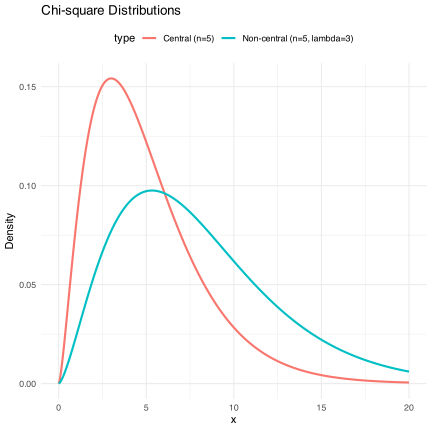
\includegraphics[keepaspectratio]{lec4-qf_files/figure-pdf/fig-plot-chisq-1.pdf}}

}

\caption{\label{fig-plot-chisq}Central vs Non-central Chi-square
Distribution}

\end{figure}%

The density of the non-central chi-square distribution shifts to the
right and becomes flatter as the non-centrality parameter \(\lambda\)
increases.

\subsection{Mean, Variance, and MGF}\label{mean-variance-and-mgf}

We summarize the key properties of the non-central chi-square
distribution.

\begin{theorem}[Properties of Non-central
Chi-square]\protect\hypertarget{thm-chisq-properties}{}\label{thm-chisq-properties}

Let \(V \sim \chi^2(n, \lambda)\). Then:

\begin{enumerate}
\def\labelenumi{\arabic{enumi}.}
\tightlist
\item
  \textbf{Mean:} \(E(V) = n + \lambda\)
\item
  \textbf{Variance:} \(\text{Var}(V) = 2n + 4\lambda\)
\item
  \textbf{Moment Generating Function (MGF):} \[
  m_V(t) = \frac{\exp\left[ -\frac{\lambda}{2} \left\{1 - \frac{1}{1-2t}\right\} \right]}{(1-2t)^{n/2}} \quad \text{for } t < 1/2
  \]
\end{enumerate}

\end{theorem}

\begin{proof}[Mean]
By definition, \(V \sim \chi^2(n, \lambda)\) is the distribution of
\(y'y\) where \(y \sim N_n(\mu, I_n)\) and the non-centrality parameter
is \(\lambda = \mu'\mu = ||\mu||^2\). Applying Lemma~\ref{lem-simple-qf}
to the random vector \(y\): \[
E(V) = E(y'y) = n + \mu'\mu = n + \lambda
\]
\end{proof}

\begin{proof}[MGF]
Since the components \(y_i\) of the vector \(y\) are independent
\(N(\mu_i, 1)\), and \(V = \sum_{i=1}^n y_i^2\), the MGF of \(V\) is the
product of the MGFs of each \(y_i^2\): \[
m_V(t) = E[e^{t \sum y_i^2}] = \prod_{i=1}^n E[e^{t y_i^2}]
\] Consider a single component \(y_i \sim N(\mu_i, 1)\). Its squared
expectation is: \[
\begin{aligned}
E[e^{t y_i^2}] &= \int_{-\infty}^{\infty} \frac{1}{\sqrt{2\pi}} e^{ty^2} e^{-\frac{1}{2}(y-\mu_i)^2} dy \\
&= \frac{1}{\sqrt{2\pi}} \int_{-\infty}^{\infty} \exp\left\{ -\frac{1}{2} \left[ (1-2t)y^2 - 2\mu_i y + \mu_i^2 \right] \right\} dy
\end{aligned}
\] Completing the square in the exponent for \(y\) (assuming
\(t < 1/2\)): \[
(1-2t)y^2 - 2\mu_i y + \mu_i^2 = (1-2t)\left(y - \frac{\mu_i}{1-2t}\right)^2 + \mu_i^2 - \frac{\mu_i^2}{1-2t}
\] The integral of the Gaussian kernel
\(\exp\{ -\frac{1}{2}(1-2t)(y - \dots)^2 \}\) yields
\(\sqrt{\frac{2\pi}{1-2t}}\). The remaining constant term is: \[
\exp\left\{ -\frac{1}{2} \left( \mu_i^2 - \frac{\mu_i^2}{1-2t} \right) \right\} = \exp\left\{ \frac{\mu_i^2}{2} \left( \frac{1}{1-2t} - 1 \right) \right\} = \exp\left\{ \frac{\mu_i^2 t}{1-2t} \right\}
\] Thus, for a single component: \[
m_{y_i^2}(t) = (1-2t)^{-1/2} \exp\left( \frac{\mu_i^2 t}{1-2t} \right)
\] Multiplying the MGFs for all \(n\) components: \[
\begin{aligned}
m_V(t) &= \prod_{i=1}^n (1-2t)^{-1/2} \exp\left( \frac{\mu_i^2 t}{1-2t} \right) \\
&= (1-2t)^{-n/2} \exp\left( \frac{t \sum \mu_i^2}{1-2t} \right)
\end{aligned}
\] Substituting \(\lambda = \sum \mu_i^2\) (so
\(\sum \mu_i^2 = \lambda\)): \[
m_V(t) = (1-2t)^{-n/2} \exp\left( \frac{\lambda t}{1-2t} \right)
\] Note that
\(\displaystyle \frac{\lambda t}{1-2t} = -\frac{\lambda}{2}\left(1 - \frac{1}{1-2t}\right)\),
which leads to the Poisson-mixture representation with
\(J \sim \text{Poisson}(\lambda/2)\).
\end{proof}

\begin{proof}[Variance]
We use the \textbf{Cumulant Generating Function},
\(K_V(t) = \ln m_V(t)\), as its derivatives yield the mean and variance
directly: \[
K_V(t) = -\frac{n}{2} \ln(1-2t) + \frac{\lambda t}{1-2t}
\] First derivative (Mean): \[
\begin{aligned}
K'_V(t) &= -\frac{n}{2} \left(\frac{-2}{1-2t}\right) + \lambda \left[ \frac{1(1-2t) - t(-2)}{(1-2t)^2} \right] \\
&= \frac{n}{1-2t} + \frac{\lambda}{(1-2t)^2}
\end{aligned}
\] Second derivative (Variance): \[
\begin{aligned}
K''_V(t) &= n(-1)(1-2t)^{-2}(-2) + \lambda(-2)(1-2t)^{-3}(-2) \\
&= \frac{2n}{(1-2t)^2} + \frac{4\lambda}{(1-2t)^3}
\end{aligned}
\] Evaluating at \(t=0\): \[
\text{Var}(V) = K''_V(0) = 2n + 4\lambda
\]
\end{proof}

\subsection{Additivity}\label{additivity}

\begin{theorem}[Additivity of
Chi-square]\protect\hypertarget{thm-chisq-additivity}{}\label{thm-chisq-additivity}

If \(v_1, \dots, v_k\) are independent random variables distributed as
\(\chi^2(n_i, \lambda_i)\), then their sum follows a chi-square
distribution:

\[
\sum_{i=1}^k v_i \sim \chi^2\left(\sum_{i=1}^k n_i, \sum_{i=1}^k \lambda_i\right)
\]

\end{theorem}

\begin{proof}
\textbf{Method 1: Using MGFs}

The moment generating function of \(v_i \sim \chi^2(n_i, \lambda_i)\)
is: \[
M_{v_i}(t) = \frac{\exp\left[-\frac{\lambda_i}{2} \left(1 - \frac{1}{1-2t}\right)\right]}{(1-2t)^{n_i/2}}
\]

Since \(v_1, \dots, v_k\) are independent, the MGF of their sum
\(V = \sum v_i\) is the product of their individual MGFs:

\[
\begin{aligned}
M_V(t) &= \prod_{i=1}^k M_{v_i}(t) \\
&= \prod_{i=1}^k \frac{\exp\left[-\frac{\lambda_i}{2} \left(1 - \frac{1}{1-2t}\right)\right]}{(1-2t)^{n_i/2}} \\
&= \frac{\exp\left[-\frac{\sum \lambda_i}{2} \left(1 - \frac{1}{1-2t}\right)\right]}{(1-2t)^{\sum n_i/2}}
\end{aligned}
\]

This is the MGF of a non-central chi-square distribution with degrees of
freedom \(\sum n_i\) and non-centrality parameter \(\sum \lambda_i\).

\textbf{Method 2: Geometric Interpretation}

Let \(v_i = ||y_i||^2\) where \(y_i \sim N_{n_i}(\mu_i, I_{n_i})\).
Since the vectors \(y_i\) are independent, we can stack them into a
larger vector \(y = (y_1', \dots, y_k')'\).

\[
y \sim N_{\sum n_i}(\mu, I_{\sum n_i}) \quad \text{where } \mu = (\mu_1', \dots, \mu_k')'
\]

The sum of squares is: \[
\sum v_i = \sum ||y_i||^2 = ||y||^2
\]

By definition, \(||y||^2\) follows a non-central chi-square distribution
with degrees of freedom equal to the dimension of \(y\) (\(\sum n_i\))
and non-centrality parameter \(\lambda = ||\mu||^2\).

\[
\lambda = \sum_{i=1}^k ||\mu_i||^2 = \sum_{i=1}^k \lambda_i
\]
\end{proof}

\subsection{Poisson Mixture
Representation}\label{poisson-mixture-representation}

\begin{theorem}[Poisson Mixture
Representation]\protect\hypertarget{thm-chisq-poisson-mixture}{}\label{thm-chisq-poisson-mixture}

Let \(v \sim \chi^2(n, \lambda)\) be a non-central chi-square random
variable. Its probability density function can be represented as a
Poisson-weighted sum of central chi-square density functions:

\[
f(v; n, \lambda) = \sum_{j=0}^{\infty} \left( \frac{e^{-\lambda/2} (\lambda/2)^j}{j!} \right) f(v; n+2j, 0)
\]

where \(f(v; \nu, 0)\) is the density of a central chi-square
distribution with \(\nu\) degrees of freedom.

\end{theorem}

\begin{proof}
We use the Moment Generating Function (MGF) approach. The MGF of a
non-central chi-square distribution \(v \sim \chi^2(n, \lambda)\) is: \[
M_v(t) = (1-2t)^{-n/2} \exp\left( \frac{\lambda}{2} \left[ \frac{1}{1-2t} - 1 \right] \right)
\]

We can expand the exponential term using the power series
\(e^x = \sum_{j=0}^\infty \frac{x^j}{j!}\): \[
\begin{aligned}
M_v(t) &= (1-2t)^{-n/2} e^{-\lambda/2} \exp\left( \frac{\lambda/2}{1-2t} \right) \\
&= e^{-\lambda/2} (1-2t)^{-n/2} \sum_{j=0}^{\infty} \frac{1}{j!} \left( \frac{\lambda/2}{1-2t} \right)^j \\
&= \sum_{j=0}^{\infty} \left( \frac{e^{-\lambda/2} (\lambda/2)^j}{j!} \right) (1-2t)^{-(n+2j)/2}
\end{aligned}
\]

Recognizing the terms:

\begin{enumerate}
\def\labelenumi{\arabic{enumi}.}
\tightlist
\item
  The term in parentheses,
  \(P(J=j) = \frac{e^{-\lambda/2} (\lambda/2)^j}{j!}\), is the
  probability mass function of a \textbf{Poisson} random variable
  \(J \sim \text{Poisson}(\lambda/2)\).
\item
  The term \((1-2t)^{-(n+2j)/2}\) is the MGF of a \textbf{central
  chi-square} distribution with \(n+2j\) degrees of freedom.
\end{enumerate}

Since the MGF of the mixture is the sum of the MGFs of the components
weighted by the mixture probabilities, the density must follow the same
mixture structure.
\end{proof}

\begin{remark}
This theorem implies a hierarchical model for generating a non-central
chi-square variable:

\begin{enumerate}
\def\labelenumi{\arabic{enumi}.}
\tightlist
\item
  Sample \(J \sim \text{Poisson}(\lambda/2)\).
\item
  Given \(J=j\), sample \(V \sim \chi^2(n+2j, 0)\).
\end{enumerate}

This is particularly useful for numerical computation, as it allows the
non-central CDF to be approximated by a finite sum of central chi-square
CDFs.
\end{remark}

\begin{figure}

\centering{

\pandocbounded{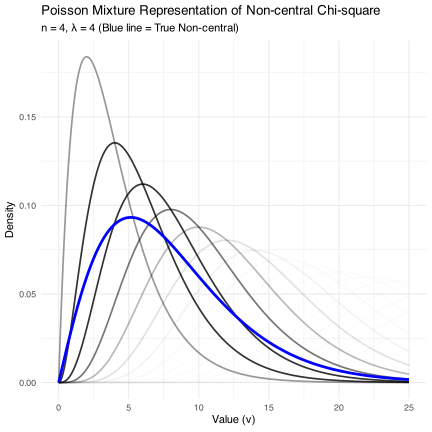
\includegraphics[keepaspectratio]{lec4-qf_files/figure-pdf/fig-chisq-poisson-mixture-fixed-1.pdf}}

}

\caption{\label{fig-chisq-poisson-mixture-fixed}The non-central
chi-square distribution as a Poisson mixture. The black curves represent
central chi-square densities with \(df = n + 2j\), with transparency
(alpha) proportional to the Poisson weight \(P(J=j)\). The solid blue
line is the true non-central chi-square density.}

\end{figure}%

\section{Distribution of Quadratic
Forms}\label{distribution-of-quadratic-forms-1}

\subsection{MGF of Quadratic Forms}\label{mgf-of-quadratic-forms}

To determine the distribution of general quadratic forms \(y'Ay\), we
look at their MGF.

\begin{theorem}[MGF of Quadratic
Form]\protect\hypertarget{thm-mgf-quad}{}\label{thm-mgf-quad}

If \(y \sim N_p(\mu, \Sigma)\), then the MGF of \(Q = y'Ay\) is:

\[
M_Q(t) = |I - 2tA\Sigma|^{-1/2} \exp\left(-\frac{1}{2} \mu' [I - (I - 2tA\Sigma)^{-1}] \Sigma^{-1} \mu\right)
\]

\end{theorem}

\subsection{Distribution of the Sum Squares of Projected Spherical
Normal}\label{distribution-of-the-sum-squares-of-projected-spherical-normal}

We will prove a simplified version of Theorem~\ref{thm-dist-quad} first.

\begin{theorem}[Distribution of Projected Spherical
Normal]\protect\hypertarget{thm-proj-matrix}{}\label{thm-proj-matrix}

If \(y \sim N_n(\mu, \sigma^2 I_n)\) and \(P_V\) is a projection matrix
onto a subspace \(V\) of dimension \(r\), then:

\[
\frac{1}{\sigma^2} y'P_V y = \frac{||P_V y||^2}{\sigma^2} \sim \chi^2\left(r, \frac{||P_V \mu||^2}{\sigma^2}\right)
\]

This holds because \(\frac{1}{\sigma^2} P_V (\sigma^2 I) = P_V\), which
is idempotent.

\end{theorem}

\begin{tcolorbox}[enhanced jigsaw, toprule=.15mm, titlerule=0mm, left=2mm, bottomrule=.15mm, opacityback=0, colback=white, leftrule=.75mm, coltitle=black, colbacktitle=quarto-callout-important-color!10!white, colframe=quarto-callout-important-color-frame, arc=.35mm, rightrule=.15mm, breakable, bottomtitle=1mm, toptitle=1mm, title=\textcolor{quarto-callout-important-color}{\faExclamation}\hspace{0.5em}{Crucial Theorem}, opacitybacktitle=0.6]

This is one of the most important theorems in the course, establishing
the fundamental conditions under which a quadratic form follows a
chi-square distribution.

\end{tcolorbox}

\begin{proof}
\textbf{When \(\sigma^2=1\)}

Let \(P_V\) be the projection matrix. We know \(P_V = QQ'\) where
\(Q = (q_1, \dots, q_r)\) is an \(n \times r\) matrix with orthonormal
columns (\(Q'Q = I_r\)).

The projection of vector \(y\) onto the subspace \(V\) can be expressed
using the orthonormal basis vectors: \[
P_V y = Q Q' y = (q_1, \dots, q_r) \begin{pmatrix} q_1' y \\ \vdots \\ q_r' y \end{pmatrix} = \sum_{i=1}^r (q_i' y) q_i
\]

The squared norm of the projection is: \[
y' P_V y = y' Q Q' y = (Q'y)' (Q'y) = ||Q'y||^2
\]

Since \(y \sim N(\mu, I_n)\), the linear transformation \(w = Q'y\)
follows: \[
w \sim N(Q'\mu, Q' I_n Q) = N(Q'\mu, I_r)
\]

Thus, \(w\) is a vector of \(r\) independent normal variables with
variance 1. The sum of squares \(||w||^2\) is by definition non-central
chi-square:

\[
||w||^2 \sim \chi^2(r, \lambda)
\] where the non-centrality parameter is: \[
\lambda = ||E(w)||^2 = ||Q'\mu||^2
\]

Note that
\(||Q'\mu||^2 = \mu' Q Q' \mu = \mu' P_V \mu = ||P_V \mu||^2\).

Thus, \(y' P_V y \sim \chi^2(r, ||P_V \mu||^2)\).

\textbf{When \(\sigma^2\not=1\)}

If \(y \sim N(\mu, \sigma^2 I_n)\), we standardize by dividing by
\(\sigma\).

Let \(w = y/\sigma\). Then \(w \sim N(\mu/\sigma, I_n)\). Applying the
previous result to \(w\):

\[
w' P_V w = \frac{y' P_V y}{\sigma^2} \sim \chi^2\left(r, \left|\left| P_V \frac{\mu}{\sigma} \right|\right|^2\right)
\] which simplifies to: \[
\frac{||P_V y||^2}{\sigma^2} \sim \chi^2\left(r, \frac{||P_V \mu||^2}{\sigma^2}\right)
\]
\end{proof}

\begin{tcolorbox}[enhanced jigsaw, toprule=.15mm, titlerule=0mm, left=2mm, bottomrule=.15mm, opacityback=0, colback=white, leftrule=.75mm, coltitle=black, colbacktitle=quarto-callout-important-color!10!white, colframe=quarto-callout-important-color-frame, arc=.35mm, rightrule=.15mm, breakable, bottomtitle=1mm, toptitle=1mm, title=\textcolor{quarto-callout-important-color}{\faExclamation}\hspace{0.5em}{Important}, opacitybacktitle=0.6]

The term \(\|P_V y\|^2\) itself is \textbf{not} a standard chi-square
variable; it is a scaled chi-square variable. Its mean is:

\[
E(\|P_V y\|^2) = \sigma^2 \left(r + \frac{\|P_V \mu\|^2}{\sigma^2}\right) = r\sigma^2 + \|P_V \mu\|^2
\]

\end{tcolorbox}

\begin{figure}[H]

{\centering \includegraphics[width=1\linewidth,height=\textheight,keepaspectratio]{lec4-qf_files/figure-pdf/plot-projection-3d-fixed-1.pdf}

}

\caption{Visualization of Projected Trivariate Normal Cloud}

\end{figure}%

\subsection{Distribution of General Quadratic
Forms}\label{distribution-of-general-quadratic-forms}

\begin{lemma}[Idempotent Matrix
Property]\protect\hypertarget{lem-idempotent-sigma}{}\label{lem-idempotent-sigma}

Let \(\Sigma\) be a positive definite matrix such that
\(\Sigma = \Sigma^{1/2}\Sigma^{1/2}\). The matrix \(A\Sigma\) is
idempotent if and only if \(\Sigma^{1/2}A\Sigma^{1/2}\) is idempotent.

\end{lemma}

\begin{proof}
\((\Rightarrow)\) Assume \(A\Sigma\) is idempotent, so
\(A\Sigma A\Sigma = A\Sigma\). Then: \[
\begin{aligned}
(\Sigma^{1/2}A\Sigma^{1/2})^2 &= \Sigma^{1/2}A(\Sigma^{1/2}\Sigma^{1/2})A\Sigma^{1/2} \\
&= \Sigma^{1/2}(A\Sigma A)\Sigma^{1/2}
\end{aligned}
\] From the assumption \(A\Sigma A\Sigma = A\Sigma\), post-multiplying
by \(\Sigma^{-1}\) gives \(A\Sigma A = A\). Substituting this back: \[
\Sigma^{1/2}(A)\Sigma^{1/2} = \Sigma^{1/2}A\Sigma^{1/2}
\]

\((\Leftarrow)\) Assume \(\Sigma^{1/2}A\Sigma^{1/2}\) is idempotent.
Then: \[
(\Sigma^{1/2}A\Sigma^{1/2})(\Sigma^{1/2}A\Sigma^{1/2}) = \Sigma^{1/2}A\Sigma^{1/2}
\] Expanding the left side: \[
\Sigma^{1/2}A(\Sigma^{1/2}\Sigma^{1/2})A\Sigma^{1/2} = \Sigma^{1/2}A\Sigma A\Sigma^{1/2}
\] Equating this to the right side: \[
\Sigma^{1/2}A\Sigma A\Sigma^{1/2} = \Sigma^{1/2}A\Sigma^{1/2}
\] Pre-multiply by \(\Sigma^{-1/2}\) and post-multiply by
\(\Sigma^{1/2}\) (which exist since \(\Sigma\) is positive definite): \[
\begin{aligned}
\Sigma^{-1/2}(\Sigma^{1/2}A\Sigma A\Sigma^{1/2})\Sigma^{1/2} &= \Sigma^{-1/2}(\Sigma^{1/2}A\Sigma^{1/2})\Sigma^{1/2} \\
I(A\Sigma A)\Sigma &= I(A)\Sigma \\
A\Sigma A\Sigma &= A\Sigma
\end{aligned}
\]
\end{proof}

\begin{lemma}[Rank
Invariance]\protect\hypertarget{lem-rank-sigma}{}\label{lem-rank-sigma}

Under the conditions of Lemma~\ref{lem-idempotent-sigma}, if \(A\Sigma\)
is idempotent, then: \[
\text{rank}(A\Sigma) = \text{rank}(\Sigma^{1/2}A\Sigma^{1/2}) = \text{tr}(A\Sigma)
\]

\end{lemma}

\begin{proof}
Since \(A\Sigma\) and \(\Sigma^{1/2}A\Sigma^{1/2}\) are both idempotent
(by Lemma~\ref{lem-idempotent-sigma}), their ranks are equal to their
traces.

Using the cyclic property of the trace operator
(\(\text{tr}(XYZ) = \text{tr}(ZXY)\)): \[
\begin{aligned}
\text{rank}(A\Sigma) &= \text{tr}(A\Sigma) \\
&= \text{tr}(A \Sigma^{1/2} \Sigma^{1/2}) \\
&= \text{tr}(\Sigma^{1/2} A \Sigma^{1/2}) \\
&= \text{rank}(\Sigma^{1/2}A\Sigma^{1/2})
\end{aligned}
\] Alternatively, notice that \(A\Sigma\) is similar to
\(\Sigma^{1/2}A\Sigma^{1/2}\): \[
A\Sigma = \Sigma^{-1/2} (\Sigma^{1/2}A\Sigma^{1/2}) \Sigma^{1/2}
\] Since similar matrices have the same rank, the equality holds.
\end{proof}

\begin{theorem}[Distribution of
y'Ay]\protect\hypertarget{thm-dist-quad}{}\label{thm-dist-quad}

Let \(y \sim N_p(\mu, \Sigma)\). Let \(A\) be a symmetric matrix of rank
\(r\). Then \(y'Ay \sim \chi^2(r, \lambda)\) with
\(\lambda = \mu' A \mu\) \textbf{if and only if} \(A\Sigma\) is
idempotent (\(A\Sigma A\Sigma = A\Sigma\)).

\textbf{Special Case (\(\Sigma = I\)):} If \(\Sigma = I\), the condition
simplifies to \(A\) being idempotent (\(A^2 = A\)).

\end{theorem}

\begin{proof}
Let \(y^* = \Sigma^{-1/2}y\), so
\(y^* \sim N_n(\Sigma^{-1/2}\mu, I_n)\). We rewrite the quadratic form:
\[y'Ay = y' \Sigma^{-1/2} (\Sigma^{1/2} A \Sigma^{1/2}) \Sigma^{-1/2} y = (y^*)' P_V y^* = \|P_V y^*\|^2\]
Since \(A\Sigma\) is idempotent, \(P_V = \Sigma^{1/2} A \Sigma^{1/2}\)
is a projection matrix with rank \(r\). By the definition of the
non-central chi-square,
\(y'Ay \sim \chi^2(r, \|P_V \Sigma^{-1/2}\mu\|^2)\). The non-centrality
parameter simplifies to \(\lambda = \mu'A\mu\).
\end{proof}

\subsection{Standardized Distance
Distribution}\label{standardized-distance-distribution}

\begin{corollary}[Standardized Distance
Distribution]\protect\hypertarget{cor-standardized-mvn}{}\label{cor-standardized-mvn}

Suppose \(y \sim N_n(\mu, \Sigma)\). Then the quadratic form
representing the standardized distance from a constant vector \(\mu_0\)
follows a non-central chi-square distribution:
\[(y-\mu_0)'\Sigma^{-1}(y-\mu_0) \sim \chi^2(n, \lambda = (\mu-\mu_0)'\Sigma^{-1}(\mu-\mu_0))\]

\end{corollary}

\begin{proof}
Let \(A = \Sigma^{-1}\). Then \(A\Sigma = \Sigma^{-1}\Sigma = I_n\),
which is clearly idempotent. Alternatively, let
\(w = \Sigma^{-1/2}(y-\mu_0)\), then
\(w \sim N_n(\Sigma^{-1/2}(\mu-\mu_0), I_n)\). By the definition of
chi-square, \(\|w\|^2 = (y-\mu_0)'\Sigma^{-1}(y-\mu_0)\) follows the
stated distribution.
\end{proof}

\begin{tcolorbox}[enhanced jigsaw, toprule=.15mm, titlerule=0mm, left=2mm, bottomrule=.15mm, opacityback=0, colback=white, leftrule=.75mm, coltitle=black, colbacktitle=quarto-callout-important-color!10!white, colframe=quarto-callout-important-color-frame, arc=.35mm, rightrule=.15mm, breakable, bottomtitle=1mm, toptitle=1mm, title=\textcolor{quarto-callout-important-color}{\faExclamation}\hspace{0.5em}{Crucial Theorem}, opacitybacktitle=0.6]

This is an important theorem we will use later.

\end{tcolorbox}

\section{Distributions of Projections of Spherical
Normal}\label{distributions-of-projections-of-spherical-normal}

\begin{theorem}[Distribution of
Projections]\protect\hypertarget{thm-proj-dist}{}\label{thm-proj-dist}

Let \(V\) be a \(k\)-dimensional subspace of \(\mathcal{R}^n\) with
projection matrix \(P_V\), and let \(y\) be a random vector in
\(\mathcal{R}^n\) with mean \(E(y)=\mu\). Then:

\begin{enumerate}
\def\labelenumi{\arabic{enumi}.}
\tightlist
\item
  \(E(P_V y) = P_V \mu\).
\item
  If \(\text{Var}(y)=\sigma^2 I_n\), then
  \(\text{Var}(P_V y) = \sigma^2 P_V\) and
  \(E(\|P_V y\|^2) = \sigma^2 k + \|P_V \mu\|^2\).
\item
  If \(y \sim N_n(\mu, \sigma^2 I_n)\), then
  \(\frac{1}{\sigma^2}\|P_V y\|^2 = \frac{1}{\sigma^2}y'P_Vy \sim \chi^2(k, \frac{1}{\sigma^2}\|P_V \mu\|^2)\).
\end{enumerate}

\end{theorem}

\begin{proof}
\leavevmode

\begin{enumerate}
\def\labelenumi{\arabic{enumi}.}
\tightlist
\item
  Since the projection operation is linear,
  \(E(P_V y) = P_V E(y) = P_V \mu\).
\item
  \(\text{Var}(P_V y) = P_V \text{Var}(y) P_V^T = P_V \sigma^2 I_n P_V = \sigma^2 P_V\).
  The expectation of the squared norm follows from the mean of a
  quadratic form:
  \(E(y'P_Vy) = \text{tr}(P_V \sigma^2 I) + \mu'P_V\mu = \sigma^2 k + \|P_V \mu\|^2\).
\item
  This is a special case of the general quadratic distribution theorem
  where \(A = \frac{1}{\sigma^2} P_V\) and \(A(\sigma^2 I) = P_V\),
  which is idempotent.
\end{enumerate}

\end{proof}

\begin{theorem}[Orthogonal
Projections]\protect\hypertarget{thm-ortho-indep}{}\label{thm-ortho-indep}

Let \(V_1, \dots, V_k\) be mutually orthogonal subspaces with dimensions
d\_i and projection matrices \(P_i\). If
\(y \sim N_n(\mu, \sigma^2 I_n)\), then:

\begin{enumerate}
\def\labelenumi{\arabic{enumi}.}
\tightlist
\item
  The projections \(\hat{y}_i = P_i y\) are independent with
  \(\hat{y}_i \sim N(P_i \mu, \sigma^2 P_i)\).
\item
  The squared norms \(\|\hat{y}_i\|^2\) are mutually independent.
\item
  \(\frac{1}{\sigma^2}\|\hat{y}_i\|^2 \sim \chi^2(d_i, \frac{1}{\sigma^2}\|P_i \mu\|^2)\).
\end{enumerate}

\end{theorem}

\begin{proof}
\leavevmode

\begin{enumerate}
\def\labelenumi{\arabic{enumi}.}
\tightlist
\item
  For \(i \ne j\), \(\text{Cov}(P_i y, P_j y) = \sigma^2 P_i P_j = 0\)
  because orthogonal projection matrices satisfy \(P_i P_j = 0\). Under
  normality, zero covariance implies independence.
\item
  Since \(\hat{y}_i\) are independent, any measurable functions of them,
  such as their squared norms, are also independent.
\item
  This follows directly from applying the projection distribution
  theorem to each independent subspace.
\end{enumerate}

\end{proof}

\subsection{Independence of Forms}\label{independence-of-forms}

\begin{theorem}[Independence
Conditions]\protect\hypertarget{thm-indep-mvn}{}\label{thm-indep-mvn}

Suppose \(y \sim N_n(\mu, \Sigma)\).

\begin{itemize}
\tightlist
\item
  \textbf{Linear and Quadratic:} \(By\) and \(y'Ay\) (where \(A\) is
  symmetric) are independent if and only if \(B\Sigma A = 0\).
\item
  \textbf{Quadratic and Quadratic:} \(y'Ay\) and \(y'By\) (where
  \(A, B\) are symmetric) are independent if and only if
  \(A\Sigma B = 0\).
\end{itemize}

\end{theorem}

\begin{proof}
If \(B\Sigma A = 0\), the normal vectors \(By\) and \(Ay\) have zero
covariance and are independent. Because \(By\) is independent of \(Ay\),
it is also independent of any measurable function of \(Ay\),
specifically \(y'Ay = \|Ay\|^2\) (if \(A\) is idempotent).
\end{proof}

\subsection{Cochran's Theorem}\label{cochrans-theorem}

\begin{theorem}[Cochran's
Result]\protect\hypertarget{thm-cochran-result}{}\label{thm-cochran-result}

Let \(y \sim N_n(\mu, \sigma^2 I)\) and \(y'y = \sum y'A_iy\). The
quadratic forms \(y^T A_i y / \sigma^2\) are mutually independent
\(\chi^2(r_i, \lambda_i)\) if and only if any one of the following
holds:

\begin{itemize}
\tightlist
\item
  Each \(A_i\) is idempotent.
\item
  \(A_i A_j = 0\) for all \(i \ne j\).
\item
  \(n = \sum r_i\).
\end{itemize}

\end{theorem}

\section{\texorpdfstring{Non-central Distributions Derived from
Non-central
\(\chi^2\)}{Non-central Distributions Derived from Non-central \textbackslash chi\^{}2}}\label{non-central-distributions-derived-from-non-central-chi2}

We begin by defining two independent Chi-squared random variables that
form the building blocks for statistical power analysis.

\begin{itemize}
\item
  \textbf{Non-central Component (\(X_1\)):}
  \(X_1 \sim \chi^2(\text{df}_1, \lambda)\). Here, \(\lambda\) is the
  non-centrality parameter, defined as the sum of squared means,
  \(\lambda = ||\mu||^2\). This is consistent with the definition used
  throughout this chapter. \emph{(Note: This definition is also used by
  R's \texttt{ncp} argument.)}
\item
  \textbf{Central Component (\(X_2\)):}
  \(X_2 \sim \chi^2(\text{df}_2)\). \(X_2\) often represents the
  \textbf{Noise Sum of Squares}, SSE\(_1\) of an adequate model, which
  is assume to follow a central \(\chi^2\),
\end{itemize}

We visualize these components as using the follow diagram.

\begin{figure}

\centering{

\pandocbounded{
\includegraphics[keepaspectratio]{lec4-qf_files/figure-pdf/fig-variance-partition-1.pdf}}

}

\caption{\label{fig-variance-partition}A diagram of two independent
\(\chi^2\) random variables}

\end{figure}%

\subsection{\texorpdfstring{The Non-central F-distribution
\(F(\text{df}_1, \text{df}_2, \lambda)\)}{The Non-central F-distribution F(\textbackslash text\{df\}\_1, \textbackslash text\{df\}\_2, \textbackslash lambda)}}\label{the-non-central-f-distribution-ftextdf_1-textdf_2-lambda}

\begin{definition}[Non-central
F]\protect\hypertarget{def-noncentral-f}{}\label{def-noncentral-f}

Let \(X_1 \sim \chi^2(\text{df}_1, \lambda)\) and
\(X_2 \sim \chi^2(\text{df}_2)\) be independent. The random variable
\(F\) follows a \textbf{non-central F-distribution}:
\[F = \frac{X_1/\text{df}_1}{X_2/\text{df}_2} \sim F(\text{df}_1, \text{df}_2, \lambda)\]

\end{definition}

\begin{itemize}
\tightlist
\item
  \textbf{Expectation:}

  \begin{itemize}
  \tightlist
  \item
    \textbf{Under \(H_0\) (\(\lambda=0\)):} Exact mean is
    \(\frac{\text{df}_2}{\text{df}_2 - 2}\) (for \(\text{df}_2 > 2\)).
  \item
    \textbf{Under \(H_1\) (\(\lambda \neq 0\)):} Approximate mean is
    \(1 + \frac{\lambda}{\text{df}_1}\).
  \end{itemize}
\end{itemize}

\begin{figure}

\centering{

\pandocbounded{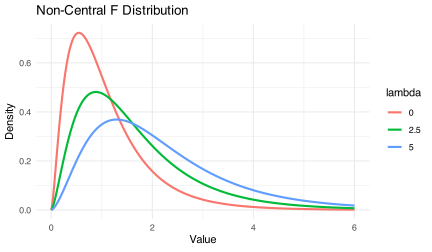
\includegraphics[keepaspectratio]{lec4-qf_files/figure-pdf/fig-nc-f-1.pdf}}

}

\caption{\label{fig-nc-f}Densities of Non-Central F (\(\lambda\) defined
as sum of squares).}

\end{figure}%

\subsection{\texorpdfstring{Type I Non-central Beta
\(\text{Beta}_1(\text{df}_1/2, \text{df}_2/2, \lambda)\)}{Type I Non-central Beta \textbackslash text\{Beta\}\_1(\textbackslash text\{df\}\_1/2, \textbackslash text\{df\}\_2/2, \textbackslash lambda)}}\label{type-i-non-central-beta-textbeta_1textdf_12-textdf_22-lambda}

\begin{definition}[Type I Non-central
Beta]\protect\hypertarget{def-noncentral-beta1}{}\label{def-noncentral-beta1}

The random variable \(B_I\) follows a \textbf{Type I non-central Beta
distribution}, defined as the signal's proportion of the total sum
(\(R^2\)):
\[B_I = \frac{X_1}{X_1 + X_2} \sim \text{Beta}_1\left(\frac{\text{df}_1}{2}, \frac{\text{df}_2}{2}, \lambda\right)\]

\end{definition}

\begin{itemize}
\tightlist
\item
  \textbf{Relationship to F:}
  \(B_I = \frac{(\text{df}_1/\text{df}_2) F}{1 + (\text{df}_1/\text{df}_2) F}\)
\item
  \textbf{Expectation:}

  \begin{itemize}
  \tightlist
  \item
    \textbf{Under \(H_0\) (\(\lambda=0\)):} Exact mean is
    \(\frac{\text{df}_1}{\text{df}_1 + \text{df}_2}\).
  \item
    \textbf{Under \(H_1\) (\(\lambda \neq 0\)):} Approximate mean is
    \(\frac{\text{df}_1 + \lambda}{\text{df}_1 + \text{df}_2 + \lambda}\).
  \end{itemize}
\end{itemize}

\begin{figure}

\centering{

\pandocbounded{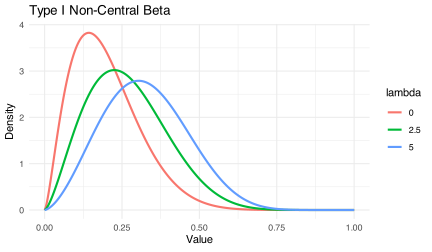
\includegraphics[keepaspectratio]{lec4-qf_files/figure-pdf/fig-nc-beta1-1.pdf}}

}

\caption{\label{fig-nc-beta1}Densities of Type I Beta (\(R^2\)).}

\end{figure}%

\subsection{\texorpdfstring{Type II Non-central Beta
\(\text{Beta}_2(\text{df}_2/2, \text{df}_1/2, \lambda)\)}{Type II Non-central Beta \textbackslash text\{Beta\}\_2(\textbackslash text\{df\}\_2/2, \textbackslash text\{df\}\_1/2, \textbackslash lambda)}}\label{type-ii-non-central-beta-textbeta_2textdf_22-textdf_12-lambda}

\begin{definition}[Type II Non-central
Beta]\protect\hypertarget{def-noncentral-beta2}{}\label{def-noncentral-beta2}

\[B_{II} = \frac{X_2}{X_1 + X_2} = 1 - B_I \sim \text{Beta}_2\left(\frac{\text{df}_2}{2}, \frac{\text{df}_1}{2}, \lambda\right)\]

\end{definition}

\begin{itemize}
\tightlist
\item
  \textbf{Relationship to F:}
  \(B_{II} = \frac{1}{1 + (\text{df}_1/\text{df}_2) F}\)
\item
  \textbf{Expectation:}

  \begin{itemize}
  \tightlist
  \item
    \textbf{Under \(H_0\) (\(\lambda=0\)):} Exact mean is
    \(\frac{\text{df}_2}{\text{df}_1 + \text{df}_2}\).
  \item
    \textbf{Under \(H_1\) (\(\lambda \neq 0\)):} Approximate mean is
    \(\frac{\text{df}_2}{\text{df}_1 + \text{df}_2 + \lambda}\).
  \end{itemize}
\end{itemize}

\begin{figure}

\centering{

\pandocbounded{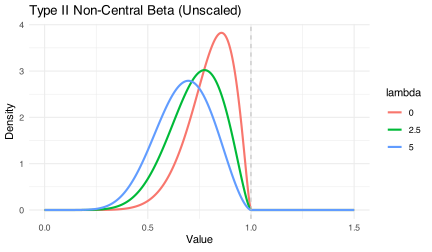
\includegraphics[keepaspectratio]{lec4-qf_files/figure-pdf/fig-beta-ii-1.pdf}}

}

\caption{\label{fig-beta-ii}Densities of Type II Beta (\(SSE/SST\)).
Support is {[}0, 1{]}.}

\end{figure}%

\subsection{\texorpdfstring{Scaled Type II Beta
\(\text{Scaled-Beta}_2(\text{df}_2/2, \text{df}_1/2, \lambda)\)}{Scaled Type II Beta \textbackslash text\{Scaled-Beta\}\_2(\textbackslash text\{df\}\_2/2, \textbackslash text\{df\}\_1/2, \textbackslash lambda)}}\label{scaled-type-ii-beta-textscaled-beta_2textdf_22-textdf_12-lambda}

\begin{definition}[Scaled Type II
Beta]\protect\hypertarget{def-scaled-beta}{}\label{def-scaled-beta}

\[S = \frac{X_2/\text{df}_2}{(X_1+X_2)/(\text{df}_1+\text{df}_2)} \sim \text{Scaled-Beta}_2\]

\end{definition}

\begin{itemize}
\tightlist
\item
  \textbf{Relationship to F:}
  \(S = \frac{\text{df}_1+\text{df}_2}{\text{df}_2 + \text{df}_1 F}\)
\item
  \textbf{Expectation:}

  \begin{itemize}
  \tightlist
  \item
    \textbf{Under \(H_0\) (\(\lambda=0\)):} Exact mean is \(1\).
  \item
    \textbf{Under \(H_1\) (\(\lambda \neq 0\)):} Approximate mean is
    \(\frac{\text{df}_1+\text{df}_2}{\text{df}_1+\text{df}_2+\lambda}\).
  \end{itemize}
\end{itemize}

\begin{figure}

\centering{

\pandocbounded{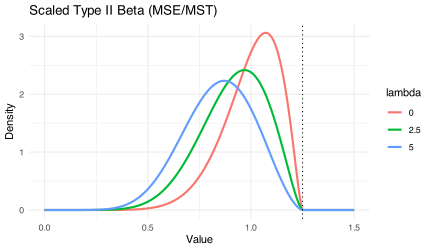
\includegraphics[keepaspectratio]{lec4-qf_files/figure-pdf/fig-scaled-beta-1.pdf}}

}

\caption{\label{fig-scaled-beta}Densities of Scaled Type II Beta
(\(MSE/MST\)).}

\end{figure}%

\subsection{\texorpdfstring{The Non-central t-distribution
\(t(\text{df}_2, \delta)\)}{The Non-central t-distribution t(\textbackslash text\{df\}\_2, \textbackslash delta)}}\label{the-non-central-t-distribution-ttextdf_2-delta}

\begin{definition}[Non-central
t]\protect\hypertarget{def-noncentral-t}{}\label{def-noncentral-t}

Let \(Z \sim N(\delta, 1)\) and \(X_2 \sim \chi^2(\text{df}_2)\) be
independent. The random variable \(T\) follows a \textbf{non-central
t-distribution}:
\[T = \frac{Z}{\sqrt{X_2/\text{df}_2}} \sim t(\text{df}_2, \delta)\]

\end{definition}

\begin{itemize}
\tightlist
\item
  \textbf{Relationship to F:} \(F = T^2\) (when \(\text{df}_1=1\)). Note
  \(\delta^2 = \lambda\).
\item
  \textbf{Expectation:}

  \begin{itemize}
  \tightlist
  \item
    \textbf{Under \(H_0\) (\(\delta=0\)):} Exact mean is \(0\).
  \item
    \textbf{Under \(H_1\) (\(\delta \neq 0\)):} Approximate mean is
    \(\delta\).
  \end{itemize}
\end{itemize}

\begin{figure}

\centering{

\pandocbounded{\includegraphics[keepaspectratio]{lec4-qf_files/figure-pdf/fig-nc-t-1.pdf}}

}

\caption{\label{fig-nc-t}Densities of Non-Central t (\(df=20\)).}

\end{figure}%

\section{Example: Inference of the Mean of Normal
Sample}\label{example-inference-of-the-mean-of-normal-sample}

Consider a random sample \(y \sim N_n(\mu j_n, \sigma^2 I_n)\). We wish
to test:

\begin{itemize}
\tightlist
\item
  \textbf{\(M_1\) (Full Model):} \(\mu\) is unknown.
\item
  \textbf{\(M_0\) (Reduced Model):} \(\mu = \mu_0\).
\end{itemize}

Let's define the transformed vector \(y^* = y - \mu_0 j_n\). Note that
\(y^* \sim N_n((\mu - \mu_0)j_n, \sigma^2 I_n)\).

\subsection{Sum of Squares and Their
Distributions}\label{sum-of-squares-and-their-distributions}

We use the projection matrix \(P_{j_n} = \frac{1}{n}j_n j_n'\) and its
complement \((I_n - P_{j_n})\) to partition the transformed vector.

\begin{itemize}
\item
  \textbf{Total SSE (\(SSE_0\) for \(M_0\)):}
  \[SSE_0 = \|I_n y^*\|^2 = \sum_{i=1}^n (Y_i - \mu_0)^2\] This follows
  a non-central distribution with \(\text{df}_{\text{total}} = n\):
  \[\frac{SSE_0}{\sigma^2} \sim \chi^2(n, \lambda) \quad \text{where } \lambda = \frac{n(\mu - \mu_0)^2}{\sigma^2}\]
\item
  \textbf{Residual SSE (\(SSE_1\) for \(M_1\)):}
  \[SSE_1 = \|(I_n - P_{j_n})y^*\|^2 = \sum_{i=1}^n (Y_i - \bar{Y})^2\]
  This captures the random noise (central component) with
  \(\text{df}_2 = n-1\): \[\frac{SSE_1}{\sigma^2} \sim \chi^2(n-1)\]
\item
  \textbf{Difference SS (\(SS_{\text{diff}}\)):}
  \[SS_{\text{diff}} = \|P_{j_n} y^*\|^2 = n(\bar{Y} - \mu_0)^2\] This
  captures the signal (non-central component) with \(\text{df}_1 = 1\):
  \[\frac{SS_{\text{diff}}}{\sigma^2} \sim \chi^2(1, \lambda)\]
\end{itemize}

\subsection{Distributions of Equivalent
Statistics}\label{distributions-of-equivalent-statistics}

We can construct five equivalent statistics to compare \(M_0\) and
\(M_1\).

\begin{itemize}
\item
  \textbf{The t-statistic (\(T\)):}
  \[T = \frac{\bar{Y} - \mu_0}{S/\sqrt{n}}\]
\item
  \textbf{The F-statistic (\(F\)):}
  \[F = \frac{n(\bar{Y} - \mu_0)^2}{S^2} = T^2\]
\item
  \textbf{The Type I Beta statistic (\(B_I\)):}
  \[B_I = \frac{SS_{\text{diff}}}{SSE_0} = \frac{n(\bar{Y} - \mu_0)^2}{\sum (Y_i - \mu_0)^2}\]
\item
  \textbf{The Type II Beta statistic (\(B_{II}\)):}
  \[B_{II} = \frac{SSE_1}{SSE_0} = \frac{\sum (Y_i - \bar{Y})^2}{\sum (Y_i - \mu_0)^2} = 1 - B_I\]
\item
  \textbf{The Scaled Type II Beta statistic (\(S_{\text{scaled}}\)):}
  \[S_{\text{scaled}} = \frac{SSE_1/(n-1)}{SSE_0/n} = \left( \frac{n}{n-1} \right) B_{II}\]
\end{itemize}

\subsection{\texorpdfstring{Expectations Under \(M_1\) and
\(M_0\)}{Expectations Under M\_1 and M\_0}}\label{expectations-under-m_1-and-m_0}

The table below contrasts the distributions and expected values of these
statistics. We assume the sample size \(n\) is large enough for the mean
of \(F\) to exist (\(n > 3\)).

\begin{itemize}
\tightlist
\item
  \textbf{Degrees of Freedom:} \(\text{df}_1 = 1\),
  \(\text{df}_2 = n-1\).
\item
  \textbf{Non-centrality:}
  \(\delta = \frac{\sqrt{n}(\mu - \mu_0)}{\sigma}\) and
  \(\lambda = \delta^2 = \frac{n(\mu - \mu_0)^2}{\sigma^2}\).
\end{itemize}

\begin{longtable}[]{@{}
  >{\raggedright\arraybackslash}p{(\linewidth - 6\tabcolsep) * \real{0.2500}}
  >{\raggedright\arraybackslash}p{(\linewidth - 6\tabcolsep) * \real{0.2500}}
  >{\raggedright\arraybackslash}p{(\linewidth - 6\tabcolsep) * \real{0.2500}}
  >{\raggedright\arraybackslash}p{(\linewidth - 6\tabcolsep) * \real{0.2500}}@{}}
\caption{Expected Values of Test Statistics Under Null and Alternative
Hypotheses}\label{tbl-expected-values}\tabularnewline
\toprule\noalign{}
\begin{minipage}[b]{\linewidth}\raggedright
Statistic
\end{minipage} & \begin{minipage}[b]{\linewidth}\raggedright
Distribution under \(H_1\) (\(\mu \neq \mu_0\))
\end{minipage} & \begin{minipage}[b]{\linewidth}\raggedright
Exact Mean under \(H_0\) (\(\mu=\mu_0\))
\end{minipage} & \begin{minipage}[b]{\linewidth}\raggedright
Approximate Mean under \(H_1\)
\end{minipage} \\
\midrule\noalign{}
\endfirsthead
\toprule\noalign{}
\begin{minipage}[b]{\linewidth}\raggedright
Statistic
\end{minipage} & \begin{minipage}[b]{\linewidth}\raggedright
Distribution under \(H_1\) (\(\mu \neq \mu_0\))
\end{minipage} & \begin{minipage}[b]{\linewidth}\raggedright
Exact Mean under \(H_0\) (\(\mu=\mu_0\))
\end{minipage} & \begin{minipage}[b]{\linewidth}\raggedright
Approximate Mean under \(H_1\)
\end{minipage} \\
\midrule\noalign{}
\endhead
\bottomrule\noalign{}
\endlastfoot
\textbf{\(T\)} & \(t(n-1, \delta)\) & \(0\) &
\(\frac{\sqrt{n}(\mu - \mu_0)}{\sigma}\) \\
\textbf{\(F\)} & \(F(1, n-1, \lambda)\) & \(\frac{n-1}{n-3} \approx 1\)
& \(1 + \frac{n(\mu - \mu_0)^2}{\sigma^2}\) \\
\textbf{\(B_I\)} &
\(\text{Beta}_1\left(\frac{1}{2}, \frac{n-1}{2}, \lambda\right)\) &
\(\frac{1}{n}\) &
\(\frac{1/n + \frac{(\mu - \mu_0)^2}{\sigma^2}}{1 + \frac{(\mu - \mu_0)^2}{\sigma^2}}\) \\
\textbf{\(B_{II}\)} &
\(\text{Beta}_2\left(\frac{n-1}{2}, \frac{1}{2}, \lambda\right)\) &
\(\frac{n-1}{n}\) &
\(\frac{(n-1)/n}{1 + \frac{(\mu - \mu_0)^2}{\sigma^2}}\) \\
\textbf{\(S_{\text{scaled}}\)} &
\(\text{Scaled-Beta}_2\left(\frac{n-1}{2}, \frac{1}{2}, \lambda\right)\)
& \(1\) & \(\frac{1}{1 + \frac{(\mu - \mu_0)^2}{\sigma^2}}\) \\
\end{longtable}

\textbf{Key Interpretation:} All statistics are functionally driven by
the signal energy. Notably, for \textbf{\(S_{\text{scaled}}\)}, the
sample size \(n\) cancels out in the approximate mean. This makes it a
direct measure of the ratio between Noise Variance and Total Variance
(Noise + Signal) in the population distributions, connected to the
Rao-Blackwell decomposition of variances.

\bookmarksetup{startatroot}

\chapter{Inference for A Multiple Linear Regression
Model}\label{inference-for-a-multiple-linear-regression-model}

\begin{center}\rule{0.5\linewidth}{0.5pt}\end{center}

\section{Linear Models and Least Square
Estimator}\label{linear-models-and-least-square-estimator}

\subsection{Assumptions in Linear
Models}\label{assumptions-in-linear-models}

Suppose that on a random sample of \(n\) units (patients, animals,
trees, etc.) we observe a response variable \(Y\) and explanatory
variables \(X_{1},...,X_{k}\). Our data are then
\((y_{i},x_{i1},...,x_{ik})\), \(i=1,...,n\), or in vector/matrix form
\(y, x_{1},...,x_{k}\) where \(y=(y_{1},...,y_{n})\) and
\(x_{j}=(x_{1j},...,x_{nj})^{T}\) or \(y, X\) where
\(X=(x_{1},...,x_{k})\).

Either by design or by conditioning on their observed values,
\(x_{1},...,x_{k}\) are regarded as vectors of known constants. The
linear model in its classical form makes the following assumptions:

\textbf{Assumptions on Linear Models}

\begin{itemize}
\item
  \textbf{A1. (Additive Error)} \(y=\mu+e\) where
  \(e=(e_{1},...,e_{n})^{T}\) is an unobserved random vector with
  \(E(e)=0\). This implies that \(\mu=E(y)\) is the unknown mean of
  \(y\).
\item
  \textbf{A2. (Linearity)}
  \(\mu=\beta_{1}x_{1}+\cdot\cdot\cdot+\beta_{k}x_{k}=X\beta\) where
  \(\beta_{1},...,\beta_{k}\) are unknown parameters. This assumption
  says that \(E(y)=\mu\in\text{Col}(X)\) (lies in the column space of
  \(X\)); i.e., it is a linear combination of explanatory vectors
  \(x_{1},...,x_{k}\) with coefficients the unknown parameters in
  \(\beta=(\beta_{1},...,\beta_{k})^{T}\). Note that it is linear in
  \(\beta_{1},...,\beta_{k}\), not necessarily in the \(x\)'s.
\item
  \textbf{A3. (Independence)} \(e_{1},...,e_{n}\) are independent random
  variables (and therefore so are \(y_{1},...,y_{n})\).
\item
  \textbf{A4. (Homoscedasticity)} \(e_{1},...,e_{n}\) all have the same
  variance \(\sigma^{2}\); that is,
  \(\text{Var}(e_{1})=\cdot\cdot\cdot=\text{Var}(e_{n})=\sigma^{2}\)
  which implies
  \(\text{Var}(y_{1})=\cdot\cdot\cdot=\text{Var}(y_{n})=\sigma^{2}\).
\item
  \textbf{A5. (Normality)} \(e\sim N_{n}(0,\sigma^{2}I_{n})\).
\end{itemize}

\subsection{Matrix Formulation}\label{matrix-formulation}

The model can be written algebraically as:
\[y_{i}=\beta_{0}+\beta_{1}x_{i1}+\beta_{2}x_{i2}+\cdot\cdot\cdot+\beta_{k}x_{ik}, \quad i=1,...,n\]

Or in matrix notation: \[
\begin{pmatrix}
y_{1}\\
y_{2}\\
\vdots\\
y_{n}
\end{pmatrix}
=
\begin{pmatrix}
1 & x_{11} & x_{12} & \cdot\cdot\cdot & x_{1k}\\
1 & x_{21} & x_{22} & \cdot\cdot\cdot & x_{2k}\\
\vdots & \vdots & \vdots & \vdots & \vdots\\
1 & x_{n1} & x_{n2} & \cdot\cdot\cdot & x_{nk}
\end{pmatrix}
\begin{pmatrix}
\beta_{0}\\
\beta_{1}\\
\vdots\\
\beta_{k}
\end{pmatrix}
+
\begin{pmatrix}
e_{1}\\
e_{2}\\
\vdots\\
e_{n}
\end{pmatrix}
\]

This is expressed compactly as: \[y=X\beta+e\] where \(X\) is the design
matrix, and \(e \sim N_n(0, \sigma^2 I)\). Alternatively:
\[y=\beta_{0}j_{n}+\beta_{1}x_{1}+\cdot\cdot\cdot+\beta_{k}x_{k}+e\]

Taken together, all five assumptions can be stated more succinctly as:
\[y\sim N_{n}(X\beta,\sigma^{2}I)\] with the mean vector
\(\mu_{y}=X\beta\in \text{Col}(X)\).

\begin{tcolorbox}[enhanced jigsaw, toprule=.15mm, titlerule=0mm, left=2mm, bottomrule=.15mm, opacityback=0, colback=white, leftrule=.75mm, coltitle=black, colbacktitle=quarto-callout-important-color!10!white, colframe=quarto-callout-important-color-frame, arc=.35mm, rightrule=.15mm, breakable, bottomtitle=1mm, toptitle=1mm, title=\textcolor{quarto-callout-important-color}{\faExclamation}\hspace{0.5em}{Coefficients and Variance of Reduced Models}, opacitybacktitle=0.6]

The effect of a parameter and the magnitude of the error variance depend
upon what other explanatory variables are present in the model. For
example, the coefficients \(\beta_{0}, \beta_{1}\) and error standard
deviation \(\sigma\) in the model:
\[y=\beta_{0}j_{n}+\beta_{1}x_{1}+\beta_{2}x_{2}+e, \quad \text{Var}(e) = \sigma^2 I\]
will typically be different than \(\beta_{0}^{*}, \beta_{1}^{*}\) and
\(\sigma^*\) in the model:
\[y=\beta_{0}^{*}j_{n}+\beta_{1}^{*}x_{1}+e^*, \quad \text{Var}(e^*) = (\sigma^*)^2 I\]
In this context, \(\beta_0^*\) and \(\beta_1^*\) are the
population-projected coefficients of the full model. Furthermore,
\(\sigma^*\) will typically be larger than \(\sigma\), as the error term
\(e^*\) absorbs the variation previously explained by \(x_2\).

\end{tcolorbox}

\begin{tcolorbox}[enhanced jigsaw, toprule=.15mm, titlerule=0mm, left=2mm, bottomrule=.15mm, opacityback=0, colback=white, leftrule=.75mm, coltitle=black, colbacktitle=quarto-callout-important-color!10!white, colframe=quarto-callout-important-color-frame, arc=.35mm, rightrule=.15mm, breakable, bottomtitle=1mm, toptitle=1mm, title=\textcolor{quarto-callout-important-color}{\faExclamation}\hspace{0.5em}{Important}, opacitybacktitle=0.6]

We will first consider the case that \(\text{rank}(X)=k+1\).

\end{tcolorbox}

\subsection{\texorpdfstring{Least Squares Estimator of \(\beta\) and
Fitted Value
\(\hat Y\)}{Least Squares Estimator of \textbackslash beta and Fitted Value \textbackslash hat Y}}\label{least-squares-estimator-of-beta-and-fitted-value-hat-y}

\begin{definition}[Least Squares
Estimator]\protect\hypertarget{def-least-squares}{}\label{def-least-squares}

The \textbf{Least Squares Estimator (LSE)} of \(\beta\), denoted as
\(\hat{\beta}\), is the vector that minimizes the Sum of Squared Errors
(SSE), which measures the discrepancy between the observed responses
\(y\) and the fitted values \(X\hat{\beta}\). \[
Q(\beta) = \sum_{i=1}^n (y_i - x_i^T \beta)^2 = (y - X\beta)'(y - X\beta)
\]

\end{definition}

\begin{theorem}[Least Squares
Estimator]\protect\hypertarget{thm-leastsquare}{}\label{thm-leastsquare}

Consider the linear model \(y = X\beta + e\), where \(X\) is of full
column rank. The Ordinary Least Squares (OLS) estimator \(\hat{\beta}\)
is given by the closed-form solution:

\[\hat{\beta} = (X'X)^{-1}X'y\]

Consequently, the vector of fitted values \(\hat{y}\) is the orthogonal
projection of \(y\) onto \(\text{Col}(X)\):

\[\hat{y} = X\hat{\beta} = Hy\]

where \(H = X(X'X)^{-1}X'\) is the orthogonal projection matrix (hat
matrix).

\end{theorem}

\begin{proof}
The derivation relies on the geometry of orthogonal projections.

\textbf{1. Obtaining the Fitted Values \(\hat{y}\)}

In the linear model, the systematic component \(E[y]\) is constrained to
lie in the column space of \(X\), denoted as \(\text{Col}(X)\). We seek
the vector in \(\text{Col}(X)\) that is ``closest'' to the observed data
\(y\). This vector is the \textbf{orthogonal projection} of \(y\) onto
\(\text{Col}(X)\), denoted as \(\hat{y}\). Using the projection matrix
\(H = X(X'X)^{-1}X'\), we have:

\[\hat{y} = Hy = X(X'X)^{-1}X' y\]

\textbf{2. Obtaining \(\hat{\beta}\) by Solving \(X\beta = \hat{y}\)}

Since \(\hat{y}\) is a projection onto \(\text{Col}(X)\), the system
\(X\hat{\beta} = \hat{y}\) is consistent. To isolate \(\hat{\beta}\), we
pre-multiply both sides by \((X'X)^{-1}X'\):

\[
\begin{aligned}
(X'X)^{-1}X' (X\hat{\beta}) &= (X'X)^{-1}X' \hat{y} \\
\underbrace{(X'X)^{-1}(X'X)}_{I} \hat{\beta} &= (X'X)^{-1}X' \hat{y} \\
\hat{\beta} &= (X'X)^{-1}X' \hat{y}
\end{aligned}
\]

Finally, we express the estimator in terms of the observed \(y\).
Because \(\hat{y}\) is an orthogonal projection, the residual
\(y - \hat{y}\) is orthogonal to the columns of \(X\), implying
\(X'\hat{y} = X'y\). Substituting this into the equation above yields
the result:

\[\hat{\beta} = (X'X)^{-1}X'y\]
\end{proof}

\subsection{\texorpdfstring{Properties of the Estimator
\(\hat \beta\)}{Properties of the Estimator \textbackslash hat \textbackslash beta}}\label{properties-of-the-estimator-hat-beta}

\begin{theorem}[Unbiasedness of
\(\hat \beta\)]\protect\hypertarget{thm-unbiased}{}\label{thm-unbiased}

If \(E(y)=X\beta\), then \(\hat{\beta}\) is an unbiased estimator for
\(\beta\).

\end{theorem}

\begin{proof}
\[
\begin{aligned}
E(\hat{\beta}) &= E[(X^{\prime}X)^{-1}X^{\prime}y] \\
&= (X^{\prime}X)^{-1}X^{\prime}E(y) \quad \text{[using linearity of expectation]} \\
&= (X^{\prime}X)^{-1}X^{\prime}X\beta \\
&= \beta
\end{aligned}
\]
\end{proof}

\begin{theorem}[Variance of
\(\hat \beta\)]\protect\hypertarget{thm-covariance}{}\label{thm-covariance}

If \(\text{Var}(y)=\sigma^{2}I\), the covariance matrix for
\(\hat{\beta}\) is given by \(\sigma^{2}(X^{\prime}X)^{-1}\).

\end{theorem}

\begin{proof}
\[
\begin{aligned}
\text{Var}(\hat{\beta}) &= \text{Var}[(X^{\prime}X)^{-1}X^{\prime}y] \\
&= (X^{\prime}X)^{-1}X^{\prime}\text{Var}(y)[(X^{\prime}X)^{-1}X^{\prime}]^{\prime} \quad \text{[using } \text{Var}(Ay) = A \text{Var}(y) A'] \\
&= (X^{\prime}X)^{-1}X^{\prime}(\sigma^{2}I)X(X^{\prime}X)^{-1} \\
&= \sigma^{2}(X^{\prime}X)^{-1}X^{\prime}X(X^{\prime}X)^{-1} \\
&= \sigma^{2}(X^{\prime}X)^{-1}
\end{aligned}
\]
\end{proof}

\textbf{Note:} These theorems require no assumption of normality.

\section{Best Linear Unbiased Estimator
(BLUE)}\label{best-linear-unbiased-estimator-blue}

\begin{theorem}[Gauss-Markov
Theorem]\protect\hypertarget{thm-gauss-markov}{}\label{thm-gauss-markov}

If \(E(y)=X\beta\) and \(\text{Var}(y)=\sigma^{2}I\), the least-squares
estimators \(\hat{\beta}_{j}, j=0,1,...,k\) have minimum variance among
all linear unbiased estimators.

\end{theorem}

\begin{proof}
We consider a linear estimator \(Ay\) of \(\beta\) and seek the matrix
\(A\) for which \(Ay\) is a minimum variance unbiased estimator.

\textbf{1. Unbiasedness Condition:} In order for \(Ay\) to be an
unbiased estimator of \(\beta\), we must have \(E(Ay)=\beta\). Using the
assumption \(E(y)=X\beta\), this is expressed as:
\[E(Ay) = A E(y) = AX\beta = \beta\] which implies the condition
\(AX=I_{k+1}\) since the relationship must hold for any \(\beta\).

\textbf{2. Minimizing Variance:} The covariance matrix for the estimator
\(Ay\) is:
\[\text{Var}(Ay) = A \text{Var}(y) A' = A(\sigma^2 I) A' = \sigma^2 AA'\]
We need to choose \(A\) (subject to \(AX=I\)) so that the diagonal
elements of \(AA'\) are minimized.

To relate \(Ay\) to \(\hat{\beta}=(X'X)^{-1}X'y\), we define
\(\hat{A} = (X'X)^{-1}X'\) and write \(A = (A - \hat{A}) + \hat{A}\).
Then: \[AA' = [(A - \hat{A}) + \hat{A}] [(A - \hat{A}) + \hat{A}]'\]
Expanding this, the cross terms vanish because
\((A - \hat{A})\hat{A}' = A\hat{A}' - \hat{A}\hat{A}'\). Note that
\(\hat{A}\hat{A}' = (X'X)^{-1}X'X(X'X)^{-1} = (X'X)^{-1}\). Also,
\(A\hat{A}' = A X (X'X)^{-1} = I (X'X)^{-1} = (X'X)^{-1}\) (since
\(AX=I\)). Thus, \((A - \hat{A})\hat{A}' = 0\).

The expansion simplifies to:
\[AA' = (A - \hat{A})(A - \hat{A})' + \hat{A}\hat{A}'\] The matrix
\((A - \hat{A})(A - \hat{A})'\) is positive semidefinite, meaning its
diagonal elements are non-negative. To minimize the diagonal of \(AA'\),
we must set \(A - \hat{A} = 0\), which implies \(A = \hat{A}\).

Thus, the minimum variance estimator is:
\[Ay = (X'X)^{-1}X'y = \hat{\beta}\]
\end{proof}

\subsection{Notes on Gauss-markov}\label{notes-on-gauss-markov}

\begin{enumerate}
\def\labelenumi{\arabic{enumi}.}
\item
  \textbf{Distributional Generality:} The remarkable feature of the
  Gauss-Markov theorem is that it holds for \emph{any} distribution of
  \(y\); normality is not required. The only assumptions used are
  linearity (\(E(y)=X\beta\)) and homoscedasticity
  (\(\text{Var}(y)=\sigma^2 I\)).
\item
  \textbf{Extension to All Linear Combinations:} The theorem extends
  beyond just the parameter vector \(\beta\) to any linear combination
  of the parameters.
\item
  \textbf{Scaling Invariance:} The predictions made by the model are
  invariant to the scaling of the explanatory variables.
\end{enumerate}

\begin{corollary}[BLUE for All Linear
Combinations]\protect\hypertarget{cor-linear-combo}{}\label{cor-linear-combo}

If \(E(y)=X\beta\) and \(\text{Var}(y)=\sigma^{2}I\), the best linear
unbiased estimator of the scalar \(a'\beta\) is \(a'\hat{\beta}\), where
\(\hat{\beta}\) is the least-squares estimator.

\end{corollary}

\begin{proof}
Let \(\tilde{\beta} = Ay\) be any other linear unbiased estimator of
\(\beta\). The variance of the linear combination \(a'\tilde{\beta}\)
is: \[
\frac{1}{\sigma^2}\text{Var}(a'\tilde{\beta}) = \frac{1}{\sigma^2}\text{Var}(a'Ay) = a'AA'a
\] From the proof of the Gauss-Markov theorem, we established that
\(AA' = (A-\hat{A})(A-\hat{A})' + (X'X)^{-1}\) where
\(\hat{A} = (X'X)^{-1}X'\). Substituting this into the variance
equation: \[
a'AA'a = a'(A-\hat{A})(A-\hat{A})'a + a'(X'X)^{-1}a
\] The term \(a'(A-\hat{A})(A-\hat{A})'a\) is a quadratic form with a
positive semidefinite matrix, so it is always non-negative. Therefore:
\[
a'AA'a \ge a'(X'X)^{-1}a = \frac{1}{\sigma^2}\text{Var}(a'\hat{\beta})
\] The variance is minimized when \(A=\hat{A}\) (specifically when the
first term is zero), proving that \(a'\hat{\beta}\) has the minimum
variance among all linear unbiased estimators.
\end{proof}

\begin{theorem}[Scaling Explanatory
Variables]\protect\hypertarget{thm-scaling}{}\label{thm-scaling}

If \(x=(1,x_{1},...,x_{k})'\) and \(z=(1,c_{1}x_{1},...,c_{k}x_{k})'\),
then the fitted values are identical:
\(\hat{y} = \hat{\beta}'x = \hat{\beta}_{z}'z\).

\end{theorem}

\begin{proof}
Let \(D = \text{diag}(1, c_1, ..., c_k)\) such that the design matrix is
transformed to \(Z = XD\). The LSE for the transformed data is: \[
\begin{aligned}
\hat{\beta}_z &= (Z'Z)^{-1}Z'y = [(XD)'(XD)]^{-1}(XD)'y \\
&= D^{-1}(X'X)^{-1}(D')^{-1}D'X'y \\
&= D^{-1}(X'X)^{-1}X'y = D^{-1}\hat{\beta}
\end{aligned}
\] . Then, the prediction is: \[
\hat{\beta}_z' z = (D^{-1}\hat{\beta})' (Dx) = \hat{\beta}' (D^{-1})' D x = \hat{\beta}'x
\] .
\end{proof}

\subsection{Limitations: Restriction to Unbiased
Estimators}\label{limitations-restriction-to-unbiased-estimators}

It is crucial to recognize that the Gauss-Markov theorem only guarantees
optimality within the class of \textbf{linear} and \textbf{unbiased}
estimators.

\begin{itemize}
\tightlist
\item
  \textbf{Assumption Sensitivity:} If the assumptions of linearity
  (\(E(y)=X\beta\)) and homoscedasticity (\(\text{Var}(y)=\sigma^2 I\))
  do not hold, \(\hat{\beta}\) may be biased or may have a larger
  variance than other estimators.
\item
  \textbf{Unbiasedness Constraint:} The theorem does not compare
  \(\hat{\beta}\) to biased estimators. It is possible for a biased
  estimator (e.g., shrinkage estimators) to have a smaller Mean Squared
  Error (MSE) than the BLUE by accepting some bias to significantly
  reduce variance. The LSE is only ``best'' (minimum variance) among
  those estimators that satisfy the unbiasedness constraint.
\end{itemize}

\section{Estimator of Error Variance}\label{estimator-of-error-variance}

We estimate \(\sigma^{2}\) by the residual mean square:

\begin{definition}[Residual Variance
Estimator]\protect\hypertarget{def-s2}{}\label{def-s2}

\[s^{2} = \frac{1}{n-k-1} \sum_{i=1}^{n}(y_{i}-x_{i}'\hat{\beta})^{2} = \frac{\text{SSE}}{n-k-1}\]
where \(\text{SSE} = (y-X\hat{\beta})'(y-X\hat{\beta})\).

\end{definition}

Alternatively, SSE can be written as:
\[\text{SSE} = y'y - \hat{\beta}'X'y\] This is often useful for
computation (\(y'y\) is the total sum of squares of the raw data).

\subsection{\texorpdfstring{Unbiasedness of
\(s^2\)}{Unbiasedness of s\^{}2}}\label{unbiasedness-of-s2}

\begin{theorem}[Unbiasedness of
s-squared]\protect\hypertarget{thm-unbiased-s2}{}\label{thm-unbiased-s2}

If \(s^{2}\) is defined as above, and if \(E(y)=X\beta\) and
\(\text{Var}(y)=\sigma^{2}I\), then \(E(s^{2})=\sigma^{2}\).

\end{theorem}

\begin{proof}
We use the Hat Matrix \(H = X(X'X)^{-1}X'\), which projects \(y\) onto
\(\text{Col}(X)\). Thus, \(\hat{y} = Hy\). The residuals are
\(y - \hat{y} = (I - H)y\). The Sum of Squared Errors is:
\[\text{SSE} = \|(I-H)y\|^2 = y'(I-H)'(I-H)y\] Since \(H\) is symmetric
and idempotent, \((I-H)\) is also symmetric and idempotent. Thus:
\[\text{SSE} = y'(I-H)y\]

To find the expectation, we use the trace trick for quadratic forms:
\(E[y'Ay] = \text{tr}(A\text{Var}(y)) + E[y]'A E[y]\). \[
\begin{aligned}
E(\text{SSE}) &= E[y'(I-H)y] \\
&= \text{tr}((I-H)\sigma^2 I) + (X\beta)'(I-H)(X\beta) \\
&= \sigma^2 \text{tr}(I-H) + \beta'X'(I-H)X\beta
\end{aligned}
\] \textbf{Trace Term:}
\(\text{tr}(I_n - H) = \text{tr}(I_n) - \text{tr}(H) = n - (k+1)\),
since
\(\text{tr}(H) = \text{tr}(X(X'X)^{-1}X') = \text{tr}((X'X)^{-1}X'X) = \text{tr}(I_{k+1}) = k+1\).

\textbf{Non-centrality Term:} Since \(HX = X\), we have \((I-H)X = 0\).
Therefore, the second term vanishes: \(\beta'X'(I-H)X\beta = 0\).

Combining these: \[E(\text{SSE}) = \sigma^2(n - k - 1)\] Dividing by the
degrees of freedom \((n-k-1)\), we get \(E(s^2) = \sigma^2\).
\end{proof}

\section{Distributions Under
Normality}\label{distributions-under-normality}

If we add Assumption A5 (\(y \sim N_n(X\beta, \sigma^2 I)\)), we can
derive the exact sampling distributions.

\begin{corollary}[Estimated Covariance of
Beta]\protect\hypertarget{cor-cov-beta}{}\label{cor-cov-beta}

An unbiased estimator of \(\text{Cov}(\hat{\beta})\) is given by:
\[\widehat{\text{Cov}}(\hat{\beta}) = s^{2}(X'X)^{-1}\]

\end{corollary}

\begin{theorem}[Sampling
Distributions]\protect\hypertarget{thm-sampling-dist}{}\label{thm-sampling-dist}

Under assumptions A1-A5:

\begin{enumerate}
\def\labelenumi{\arabic{enumi}.}
\tightlist
\item
  \(\hat{\beta} \sim N_{k+1}(\beta, \sigma^{2}(X'X)^{-1})\).
\item
  \((n-k-1)s^{2}/\sigma^{2} \sim \chi^{2}(n-k-1)\).
\item
  \(\hat{\beta}\) and \(s^{2}\) are independent.
\end{enumerate}

\end{theorem}

\begin{proof}
\textbf{Part (i):} Since \(\hat{\beta} = (X'X)^{-1}X'y\) is a linear
transformation of the normal vector \(y\), it is also normally
distributed. We already established its mean and variance in
Theorem~\ref{thm-unbiased} and Theorem~\ref{thm-covariance}.

\textbf{Part (ii):} We showed \(\text{SSE} = y'(I-H)y\). Since \((I-H)\)
is idempotent with rank \(n-k-1\), and \((I-H)X\beta = 0\), by the
theory of quadratic forms in normal variables,
\(\text{SSE}/\sigma^2 \sim \chi^2(n-k-1)\).

\textbf{Part (iii):} \(\hat{\beta}\) depends on \(Hy\) (or \(X'y\)),
while \(s^2\) depends on \((I-H)y\). Since \(H(I-H) = H - H^2 = 0\), the
linear forms defining the estimator and the residuals are orthogonal.
For normal vectors, zero covariance implies independence.
\end{proof}

\section{Maximum Likelihood Estimator
(MLE)}\label{maximum-likelihood-estimator-mle}

\begin{theorem}[MLE for Linear
Regression]\protect\hypertarget{thm-mle}{}\label{thm-mle}

If \(y \sim N_n(X\beta, \sigma^2 I)\), the Maximum Likelihood Estimators
are: \[
\hat{\beta}_{\text{MLE}} = (X'X)^{-1}X'y
\] \[
\hat{\sigma}^2_{\text{MLE}} = \frac{1}{n}(y - X\hat{\beta})'(y - X\hat{\beta}) = \frac{\text{SSE}}{n}
\]

\end{theorem}

\begin{proof}
The log-likelihood function is:
\[ \ln L(\beta, \sigma^2) = -\frac{n}{2}\ln(2\pi) - \frac{n}{2}\ln(\sigma^2) - \frac{1}{2\sigma^2}(y - X\beta)'(y - X\beta) \]
Maximizing this with respect to \(\beta\) is equivalent to minimizing
the quadratic term \((y - X\beta)'(y - X\beta)\), which yields the Least
Squares Estimator. Differentiating with respect to \(\sigma^2\) and
setting to zero yields \(\hat{\sigma}^2 = \text{SSE}/n\).
\end{proof}

\textbf{Note:} The MLE for \(\sigma^2\) is biased (denominator \(n\)),
whereas \(s^2\) is unbiased (denominator \(n-k-1\)).

\section{Linear Models in Centered
Form}\label{linear-models-in-centered-form}

The regression model can be written in a centered form by subtracting
the means of the explanatory variables:
\[y_{i}=\alpha+\beta_{1}(x_{i1}-\overline{x}_{1})+\beta_{2}(x_{i2}-\overline{x}_{2})+\cdot\cdot\cdot+\beta_{k}(x_{ik}-\overline{x}_{k})+e_{i}\]
for \(i=1,...,n\), where the intercept term is adjusted:
\[\alpha=\beta_{0}+\beta_{1}\overline{x}_{1}+\beta_{2}\overline{x}_{2}+\cdot\cdot\cdot+\beta_{k}\overline{x}_{k}\]
and \(\overline{x}_{j}=\frac{1}{n}\sum_{i=1}^{n}x_{ij}\).

\subsection{Matrix Formulation}\label{matrix-formulation-1}

In matrix form, the equivalence between the original model and the
centered model is:
\[y = X\beta + e = (j_n, X_c)\begin{pmatrix} \alpha \\ \beta_{1} \end{pmatrix} + e\]
where \(\beta_{1}=(\beta_{1},...,\beta_{k})^{T}\) represents the slope
coefficients, and \(X_c\) is the centered design matrix:
\[X_c = (I - P_{j_n})X_1\] Here, \(X_1\) consists of the original
columns of \(X\) excluding the intercept column.

To see the structure of \(X_c\), we first calculate the projection of
the data onto the intercept space, \(P_{j_n}X_1\): \[
\begin{aligned}
P_{j_n}X_1 &= \frac{1}{n}j_n j_n' X_1 \\
&= \begin{pmatrix} 1/n & 1/n & \cdots & 1/n \\ 1/n & 1/n & \cdots & 1/n \\ \vdots & \vdots & \ddots & \vdots \\ 1/n & 1/n & \cdots & 1/n \end{pmatrix} \begin{pmatrix} x_{11} & x_{12} & \cdots & x_{1k} \\ x_{21} & x_{22} & \cdots & x_{2k} \\ \vdots & \vdots & \ddots & \vdots \\ x_{n1} & x_{n2} & \cdots & x_{nk} \end{pmatrix} \\
&= \begin{pmatrix} \bar{x}_1 & \bar{x}_2 & \cdots & \bar{x}_k \\ \bar{x}_1 & \bar{x}_2 & \cdots & \bar{x}_k \\ \vdots & \vdots & \ddots & \vdots \\ \bar{x}_1 & \bar{x}_2 & \cdots & \bar{x}_k \end{pmatrix}
\end{aligned}
\] This results in a matrix where every row is the vector of column
means. Subtracting this from \(X_1\) gives \(X_c\): \[
\begin{aligned}
X_c &= X_1 - P_{j_n}X_1 \\
&= \begin{pmatrix} x_{11} & x_{12} & \cdots & x_{1k} \\ x_{21} & x_{22} & \cdots & x_{2k} \\ \vdots & \vdots & \ddots & \vdots \\ x_{n1} & x_{n2} & \cdots & x_{nk} \end{pmatrix} - \begin{pmatrix} \bar{x}_1 & \bar{x}_2 & \cdots & \bar{x}_k \\ \bar{x}_1 & \bar{x}_2 & \cdots & \bar{x}_k \\ \vdots & \vdots & \ddots & \vdots \\ \bar{x}_1 & \bar{x}_2 & \cdots & \bar{x}_k \end{pmatrix} \\
&= \begin{pmatrix} x_{11} - \bar{x}_1 & x_{12} - \bar{x}_2 & \cdots & x_{1k} - \bar{x}_k \\ x_{21} - \bar{x}_1 & x_{22} - \bar{x}_2 & \cdots & x_{2k} - \bar{x}_k \\ \vdots & \vdots & \ddots & \vdots \\ x_{n1} - \bar{x}_1 & x_{n2} - \bar{x}_2 & \cdots & x_{nk} - \bar{x}_k \end{pmatrix}
\end{aligned}
\]

\subsection{Estimation in Centered
Form}\label{estimation-in-centered-form}

Because the column space of the intercept \(j_n\) is orthogonal to the
columns of \(X_c\) (since columns of \(X_c\) sum to zero), the
cross-product matrix becomes block diagonal: \[
\begin{pmatrix} j_n' \\ X_c' \end{pmatrix} (j_n, X_c) = \begin{pmatrix} j_n'j_n & j_n'X_c \\ X_c'j_n & X_c'X_c \end{pmatrix} = \begin{pmatrix} n & 0 \\ 0 & X_c'X_c \end{pmatrix}
\]

\begin{theorem}[Centered
Estimators]\protect\hypertarget{thm-centered-estimators}{}\label{thm-centered-estimators}

The least squares estimators for the centered parameters are: \[
\begin{pmatrix} \hat{\alpha} \\ \hat{\beta}_{1} \end{pmatrix} = \begin{pmatrix} n & 0 \\ 0 & X_c'X_c \end{pmatrix}^{-1} \begin{pmatrix} j_n'y \\ X_c'y \end{pmatrix} = \begin{pmatrix} \bar{y} \\ (X_c'X_c)^{-1}X_c'y \end{pmatrix}
\] Thus:

\begin{enumerate}
\def\labelenumi{\arabic{enumi}.}
\tightlist
\item
  \(\hat{\alpha} = \bar{y}\) (The sample mean of \(y\)).
\item
  \(\hat{\beta}_{1} = S_{xx}^{-1}S_{xy}\), using the sample covariance
  notations.
\end{enumerate}

\end{theorem}

Recovering the original intercept:
\[ \hat{\beta}_0 = \hat{\alpha} - \hat{\beta}_1 \bar{x}_1 - \dots - \hat{\beta}_k \bar{x}_k = \bar{y} - \hat{\beta}_{1}'\bar{x} \]

\section{Decomposition of Sum of
Squares}\label{decomposition-of-sum-of-squares}

We partition the total variation based on the orthogonal subspaces.

\begin{definition}[Sum of Squares
Components]\protect\hypertarget{def-ss-components}{}\label{def-ss-components}

The total variation is decomposed as
\(\text{SST} = \text{SSR} + \text{SSE}\).

\begin{enumerate}
\def\labelenumi{\arabic{enumi}.}
\item
  \textbf{Total Sum of Squares (SST):} The squared length of the
  centered response vector.
  \[\text{SST} = \|y - \bar{y}j_n\|^2 = \|(I - P_{j_n})y\|^2\]
\item
  \textbf{Regression Sum of Squares (SSR):} The variation explained by
  the regressors \(X_c\).
  \[\text{SSR} = \|\hat{y} - \bar{y}j_n\|^2 = \|P_{X_c}y\|^2 = \hat{\beta}_1' X_c' X_c \hat{\beta}_1\]
\item
  \textbf{Sum of Squared Errors (SSE):} The residual variation.
  \[\text{SSE} = \|y - \hat{y}\|^2 = \|(I - H)y\|^2\]
\end{enumerate}

\end{definition}

\subsection{\texorpdfstring{3D Visualization of Decomposition of
\(y\)}{3D Visualization of Decomposition of y}}\label{d-visualization-of-decomposition-of-y}

We partition the total variation in \(y\) based on the orthogonal
subspaces.

\begin{enumerate}
\def\labelenumi{\arabic{enumi}.}
\tightlist
\item
  \textbf{Space of the Mean:} \(L(j_n)\), spanned by the intercept
  vector \(j_n\).
\item
  \textbf{Space of the Regressors:} \(L(X_c)\), spanned by the centered
  predictors \(X_c\).
\item
  \textbf{Error Space:} \(\text{Col}(X)^\perp\), orthogonal to the model
  space.
\end{enumerate}

The vector \(y\) can be decomposed into three orthogonal components:
\[y = \bar{y}j_n + P_{X_c}y + (y - \hat{y})\] Visually, this corresponds
to projecting the vector \(y\) onto three orthogonal axes.

\textbf{Interactive Visualization:}

We generate a cloud of 100 observations of \(y\) from
\(N(\mu, \sigma=1)\) where \(\mu = (5,5,0)\). The projections onto the
Model Plane (\(z=0\)) are highlighted in \textbf{red}, and the
projections onto the error axis (\(z\)) are in \textbf{yellow}.

\subsubsection{Effect Exists (signal)}

\begin{figure}[H]

{\centering \includegraphics[width=1\linewidth,height=\textheight,keepaspectratio]{figs/geometry-3d-signal.png}

}

\caption{Scenario 1: Significant regression effect (\(\beta_1
ot= 0\)). The mean vector projects significantly onto the predictor
space.}

\end{figure}%

\subsubsection{No Effect (noise)}

\begin{figure}[H]

{\centering \includegraphics[width=1\linewidth,height=\textheight,keepaspectratio]{figs/geometry-3d-noise.png}

}

\caption{Scenario 2: No regression effect (\(\beta_1 = 0\)). The mean
vector lies purely on the intercept axis.}

\end{figure}%

\subsection{A Diagram to Show Decomposition of Sum of
Squares}\label{a-diagram-to-show-decomposition-of-sum-of-squares}

The decomposition of the total variation is visualized below. The total
deviation (Orange) is the vector sum of the regression deviation (Green)
and the residual error (Red).

\begin{figure}

\centering{

\pandocbounded{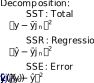
\includegraphics[keepaspectratio]{lec5-est_files/figure-pdf/fig-ss-decomposition-legend-v2-1.pdf}}

}

\caption{\label{fig-ss-decomposition-legend-v2}Geometric Decomposition:
SST = SSR + SSE}

\end{figure}%

\subsection{Distribution of Sum of
Squares}\label{distribution-of-sum-of-squares}

We apply the general theory of projections to the specific components
defined in Definition~\ref{def-ss-components}.

\begin{theorem}[Distribution of Sum of
Squares]\protect\hypertarget{thm-distribution-ss-v2}{}\label{thm-distribution-ss-v2}

Let \(y \sim N(\mu, \sigma^2 I_n)\), where \(\mu \in \text{Col}(X)\).
Consider the decomposition defined by the projection matrices
\(P_{X_c}\) and \(M = I - H\).

\begin{itemize}
\item
  \textbf{Independence:} The quadratic forms \(\text{SSR}\) and
  \(\text{SSE}\) are statistically independent because the subspaces
  \(L(X_c)\) and \(\text{Col}(X)^\perp\) are orthogonal.
\item
  \textbf{Distribution of SSE:} The scaled sum of squared errors follows
  a central Chi-squared distribution:
  \[ \frac{\text{SSE}}{\sigma^2} = \frac{\|(I - H)y\|^2}{\sigma^2} \sim \chi^2(n-k-1) \]
  \textbf{Mean:} \[ E[\text{SSE}] = \sigma^2(n-k-1) \]
\item
  \textbf{Distribution of SSR:} The scaled regression sum of squares
  follows a \textbf{non-central} Chi-squared distribution:
  \[ \frac{\text{SSR}}{\sigma^2} = \frac{\|P_{X_c}y\|^2}{\sigma^2} \sim \chi^2(k, \lambda) \]
  \textbf{Mean:} \[ E[\text{SSR}] = \sigma^2 k + \|P_{X_c}\mu\|^2 \]
\end{itemize}

\textbf{Non-centrality Parameter (\(\lambda\)):}
\[ \lambda = \frac{1}{\sigma^2} \|P_{X_c} \mu\|^2 \] where
\[\|P_{X_c} \mu\|^2 = \|X_c \beta_1\|^2 = (X_c \beta_1)' (X_c \beta_1) = \beta_1' X_c' X_c \beta_1\]

\end{theorem}

\begin{proof}
We apply Theorem~\ref{thm-proj-dist} to the specific projection matrices
identified in the definitions.

\begin{itemize}
\item
  \textbf{For SSE (Error Space):} \(\text{SSE}\) is defined by the
  projection matrix \(P_V = I - H\).

  \begin{itemize}
  \tightlist
  \item
    \textbf{Dimension:} The rank of \((I - H)\) is
    \(n - \text{rank}(X) = n - (k+1) = n - k - 1\).
  \item
    \textbf{Non-centrality:} Since \(\mu \in \text{Col}(X)\), the
    projection onto the orthogonal complement is zero:
    \(\|(I - H)\mu\|^2 = 0\). Thus, \(\lambda = 0\).
  \item
    \textbf{Expectation:} Using Part 2 of Theorem~\ref{thm-proj-dist}
    (\(E(\|P_V y\|^2) = \sigma^2 \text{rank}(P_V) + \|P_V \mu\|^2\)):
    \[ E[\text{SSE}] = \sigma^2(n-k-1) + 0 = \sigma^2(n-k-1) \]
  \end{itemize}
\item
  \textbf{For SSR (Regression Space):} \(\text{SSR}\) is defined by the
  projection matrix \(P_V = P_{X_c}\).

  \begin{itemize}
  \item
    \textbf{Dimension:} The rank of \(P_{X_c}\) is \((k+1) - 1 = k\).
  \item
    \textbf{Non-centrality:} The projection of \(\mu\) onto \(L(X_c)\)
    is \(P_{X_c}\mu\).
    \[ \lambda = \frac{1}{2\sigma^2} \|P_{X_c} \mu\|^2 \]
  \item
    \textbf{Expectation:} Using Part 2 of Theorem~\ref{thm-proj-dist}:
    \[ E[\text{SSR}] = \sigma^2 k + \|P_{X_c}\mu\|^2 \]
  \end{itemize}

  This shows that while \(E[\text{SSE}]\) depends only on the noise
  variance and sample size, \(E[\text{SSR}]\) is inflated by the
  magnitude of the true regression signal \(\|P_{X_c}\mu\|^2\).
\end{itemize}

\end{proof}

\section{F-test for Testing Overall Regression
Effect}\label{f-test-for-testing-overall-regression-effect}

We wish to test whether the regression model provides any explanatory
power beyond the simple intercept-only model.

\textbf{Hypotheses:}

\begin{itemize}
\item
  \textbf{Null Hypothesis (\(H_0\)):}
  \(\beta_1 = \beta_2 = \dots = \beta_k = 0\) (No regression effect).
  This implies \(\mu \in \text{span}(j_n)\) and the true signal variance
  \(\|X_c\beta_1\|^2 = 0\).
\item
  \textbf{Alternative Hypothesis (\(H_1\)):} At least one
  \(\beta_j \neq 0\).
\end{itemize}

\subsection*{The F-statistic}\label{the-f-statistic}
\addcontentsline{toc}{subsection}{The F-statistic}

We construct the test statistic using the ratio of the Mean Squares
defined previously:

\[F = \frac{\text{MSR}}{\text{MSE}} = \frac{\text{SSR}/k}{\text{SSE}/(n-k-1)}\]

\subsection*{\texorpdfstring{Understanding \(F\) via
Expectations}{Understanding F via Expectations}}\label{understanding-f-via-expectations}
\addcontentsline{toc}{subsection}{Understanding \(F\) via Expectations}

The logic of the F-test is transparent when we examine the expected
values of the numerator and denominator:

\[
\begin{aligned}
E[\text{MSE}] &= \sigma^2 \\
E[\text{MSR}] &= \sigma^2 + \frac{\|X_c \beta_1\|^2}{k}
\end{aligned}
\]

\begin{itemize}
\tightlist
\item
  \textbf{If \(H_0\) is true:} The signal term is zero. Both Mean
  Squares estimate \(\sigma^2\) unbiasedly. We expect \(F \approx 1\).
\item
  \textbf{If \(H_1\) is true:} The numerator includes the positive term
  \(\frac{\|X_c \beta_1\|^2}{k}\). We expect \(F > 1\).
\end{itemize}

Therefore, we reject \(H_0\) for sufficiently large values of \(F\).
Specifically, we reject at level \(\alpha\) if
\(F_{obs} > F_{\alpha}(k, n-k-1)\).

\subsection{Distributional Theory}\label{distributional-theory}

To derive the exact sampling distribution, we rely on the independence
of the sums of squares (from Theorem~\ref{thm-distribution-ss-v2}) and
the definition of the non-central F-distribution given in
\textbf{Definition~\ref{def-noncentral-f}}.

\begin{theorem}[Distribution of Regression
F-Statistic]\protect\hypertarget{thm-regression-f-dist}{}\label{thm-regression-f-dist}

Under the assumption of normality, the regression F-statistic follows a
\textbf{non-central F-distribution}:

\[ F \sim F(k, n-k-1, \lambda) \]

The non-centrality parameter \(\lambda\) is determined by the ratio of
the signal sum of squares to the error variance:
\[ \lambda = \frac{\|X_c \beta_1\|^2}{\sigma^2} \]

\textbf{Special Cases:}

\begin{enumerate}
\def\labelenumi{\arabic{enumi}.}
\tightlist
\item
  \textbf{Under \(H_1\) (Signal exists):} \(\lambda > 0\), so \(F\)
  follows the non-central distribution.
\item
  \textbf{Under \(H_0\) (No signal):}
  \(\beta_1 = 0 \implies \lambda = 0\). The distribution collapses to
  the \textbf{central F-distribution}: \[ F \sim F(k, n-k-1) \]
\end{enumerate}

\end{theorem}

\begin{proof}
We identify the components from Definition~\ref{def-noncentral-f}:

\begin{enumerate}
\def\labelenumi{\arabic{enumi}.}
\tightlist
\item
  \textbf{Numerator (\(X_1\)):} Let \(X_1 = \text{SSR}/\sigma^2\). From
  Theorem~\ref{thm-distribution-ss-v2}, \(X_1 \sim \chi^2(k, \lambda)\).
\item
  \textbf{Denominator (\(X_2\)):} Let \(X_2 = \text{SSE}/\sigma^2\).
  From Theorem~\ref{thm-distribution-ss-v2}, \(X_2 \sim \chi^2(n-k-1)\).
\item
  \textbf{Independence:} \(X_1\) and \(X_2\) are independent.
\end{enumerate}

Substituting these into the F-statistic: \[
F = \frac{\text{MSR}}{\text{MSE}} = \frac{(\text{SSR}/\sigma^2)/k}{(\text{SSE}/\sigma^2)/(n-k-1)} = \frac{X_1/k}{X_2/(n-k-1)}
\] By definition Definition~\ref{def-noncentral-f}, this ratio follows
\(F(k, n-k-1, \lambda)\).
\end{proof}

\subsection{Visualization of the Rejection
Region}\label{visualization-of-the-rejection-region}

The following plot illustrates the central F-distribution (valid under
\(H_0\)) for \(k=3\) predictors and \(n=20\) observations
(\(df_1 = 3, df_2 = 16\)). An observed statistic of \(F=2\) is marked,
with the p-value represented by the shaded tail area.

\begin{figure}

\centering{

\pandocbounded{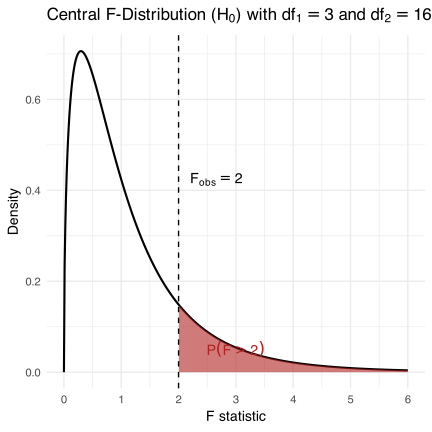
\includegraphics[keepaspectratio]{lec5-est_files/figure-pdf/fig-f-dist-example-1.pdf}}

}

\caption{\label{fig-f-dist-example}Probability Density Function of F(3,
16) under H0. The shaded region represents the p-value.}

\end{figure}%

\section{\texorpdfstring{Raw Coefficient of Determination
(\(R^2\))}{Raw Coefficient of Determination (R\^{}2)}}\label{raw-coefficient-of-determination-r2}

\subsection{Definition}\label{definition}

The \(R^2\) statistic measures the proportion of total variation
explained by the regression model.

\begin{definition}[R-Squared]\protect\hypertarget{def-r2}{}\label{def-r2}

\[R^2 = \frac{\text{SSR}}{\text{SST}} = 1 - \frac{\text{SSE}}{\text{SST}}\]
Since \(0 \le \text{SSE} \le \text{SST}\), it follows that
\(0 \le R^2 \le 1\).

\end{definition}

\subsection{Expectation and Bias}\label{expectation-and-bias}

To understand the bias in \(R^2\), it is more illuminating to analyze
the expectation of the \textbf{unexplained variance} (\(1 - R^2\)). This
term represents the ratio of error sum of squares to the total sum of
squares:

\[ E[1 - R^2] = E\left[ \frac{\text{SSE}}{\text{SST}} \right] \]

Using the first-order approximation \(E[X/Y] \approx E[X]/E[Y]\), we
examine the numerator and denominator separately:

\[
\begin{aligned}
E[\text{SSE}] &= \sigma^2(n-k-1) \\
E[\text{SST}] &= \sigma^2(n-1) + \sigma^2\lambda = \sigma^2 \left( (n-1) + \frac{\|X_c \beta_1\|^2}{\sigma^2} \right)
\end{aligned}
\]

Substituting these back, we approximate the expected unexplained
fraction:

\[ E[1 - R^2] \approx \frac{\sigma^2(n-k-1)}{\sigma^2 \left( (n-1) + \frac{\|X_c \beta_1\|^2}{\sigma^2} \right)} = \frac{n-k-1}{(n-1) + \frac{\|X_c \beta_1\|^2}{\sigma^2}} \]

\textbf{Behavior under Null Hypothesis (\(H_0\)):} When there is no true
signal (\(\beta_1 = 0\)), the term
\(\frac{\|X_c \beta_1\|^2}{\sigma^2}\) vanishes. The expected proportion
of unexplained variance becomes:

\[ E[1 - R^2 | H_0] \approx \frac{n-k-1}{n-1} \]

\begin{tcolorbox}[enhanced jigsaw, toprule=.15mm, titlerule=0mm, left=2mm, bottomrule=.15mm, opacityback=0, colback=white, leftrule=.75mm, coltitle=black, colbacktitle=quarto-callout-note-color!10!white, colframe=quarto-callout-note-color-frame, arc=.35mm, rightrule=.15mm, breakable, bottomtitle=1mm, toptitle=1mm, title=\textcolor{quarto-callout-note-color}{\faInfo}\hspace{0.5em}{Note}, opacitybacktitle=0.6]

This result reveals the source of the bias:

\begin{enumerate}
\def\labelenumi{\arabic{enumi}.}
\tightlist
\item
  Ideally, if predictors are noise, the model should explain nothing,
  and \(E[1-R^2]\) should be \(1\).
\item
  Instead, the expected error ratio is \textbf{less than 1},
  specifically scaled by \(\frac{n-k-1}{n-1}\).
\item
  This scaling factor is exactly what the \textbf{Adjusted R-squared
  (\(R^2_a\))} attempts to correct by multiplying the observed ratio by
  the inverse \(\frac{n-1}{n-k-1}\).
\end{enumerate}

\end{tcolorbox}

\subsection{Exact Distribution}\label{exact-distribution}

The \(R^2\) statistic follows the Type I Non-central Beta distribution
derived from the ratio of independent Chi-squared variables.

\begin{theorem}[Distribution of
R-Squared]\protect\hypertarget{thm-r2-dist}{}\label{thm-r2-dist}

\[ R^2 \sim \text{Beta}_1\left( \frac{k}{2}, \frac{n-k-1}{2}, \lambda \right) \]
where \(\text{df}_1 = k\) and \(\text{df}_2 = n-k-1\).

\end{theorem}

\section{\texorpdfstring{Adjusted R-squared
(\(R^2_a\))}{Adjusted R-squared (R\^{}2\_a)}}\label{adjusted-r-squared-r2_a}

To correct for the inflation of \(R^2\) due to model complexity (\(k\)),
we introduce the Adjusted \(R^2\). This statistic penalizes the sum of
squares by their degrees of freedom:

\[ R^2_a = 1 - \frac{\text{SSE}/(n-k-1)}{\text{SST}/(n-1)} = 1 - \frac{\text{MSE}}{\text{MST}} = 1 - (1 - R^2) \frac{n-1}{n-k-1} \]

\textbf{Expectation:}

Under \(H_0\), since \(E[\text{MSE}] = E[\text{MST}] = \sigma^2\), the
estimator is asymptotically unbiased:

\[ E[R^2_a | H_0] \approx 0 \]

\textbf{Variance and Stability:}

While \(R^2_a\) corrects the bias, it introduces instability. The
variance of \(R^2_a\) under \(H_0\) can be derived from the variance of
the Beta distribution:

\[ \text{Var}(R^2_a | H_0) = \left( \frac{n-1}{n-k-1} \right)^2 \text{Var}(R^2 | H_0) \]

Substituting \(\text{Var}(R^2 | H_0) = \frac{2k(n-k-1)}{(n-1)^2(n+1)}\),
we obtain:

\[ \text{Var}(R^2_a | H_0) = \frac{2k}{(n-k-1)(n+1)} \]

\textbf{Key Insight:}

As the model complexity \(k\) increases relative to \(n\):

\begin{enumerate}
\def\labelenumi{\arabic{enumi}.}
\tightlist
\item
  The denominator \((n-k-1)\) shrinks.
\item
  The variance \(\text{Var}(R^2_a)\) explodes.
\end{enumerate}

This implies that for high-dimensional models (large \(k/n\)), \(R^2_a\)
becomes an extremely noisy estimator, often yielding large negative
values even for null models.

\section{\texorpdfstring{Population Proportion of Signals
(\(\rho^2\))}{Population Proportion of Signals (\textbackslash rho\^{}2)}}\label{population-proportion-of-signals-rho2}

The formula for the expected Adjusted \(R^2\) reveals a deep connection
to the decomposition of variance in population quantities. Recall the
Rao-Blackwell theorem (or Law of Total Variance), which decomposes the
total variance of a single observation \(Y_i\) into the expected
conditional variance (noise) and the variance of the conditional
expectation (signal). Let \(\sigma^2_\mu\) denote the signal variance
and \(\sigma^2\) denote the noise variance:

\[ \text{Var}(Y_i) = E[\text{Var}(Y_i|x_{(i)})] + \text{Var}(E[Y_i|x_{(i)}]) \]
\[ \sigma^2_Y = \sigma^2 + \sigma^2_\mu \]

In our derived expectation for \(R^2_a\):
\[ E[R^2_a] \approx \frac{\frac{\|X_c\beta_1\|^2}{n-1}}{\sigma^2 + \frac{\|X_c\beta_1\|^2}{n-1}} \]

The term in the numerator, \(\frac{\|X_c\beta_1\|^2}{n-1}\), is
precisely the \textbf{sample variance of the true means} \(\mu_i\). Let
\(\mu = X\beta\). We can expand the centered signal vector
\(X_c\beta_1\) to see this explicitly. Since \(\mu \in \text{Col}(X)\),
we know \(H\mu = \mu\):

\[
X_c\beta_1 = P_{X_c} \mu = (H - P_{j_n})\mu = H\mu - P_{j_n}\mu = \mu - \bar{\mu}j_n = 
\begin{pmatrix} 
\mu_1 - \bar{\mu} \\ 
\mu_2 - \bar{\mu} \\ 
\vdots \\ 
\mu_n - \bar{\mu} 
\end{pmatrix}
\]

This vector represents the deviation of each observation's true mean
from the grand mean. Consequently, the squared norm divided by degrees
of freedom is:
\[ \frac{\|X_c\beta_1\|^2}{n-1} = \frac{\sum_{i=1}^n (\mu_i - \bar{\mu})^2}{n-1} = \sigma^2_\mu \]

Thus, \(R^2_a\) is therefore an unbiased estimator for the
\textbf{proportion of variance explained by the signal} in the
population:
\[ E[R^2_a] \approx \frac{\sigma^2_\mu}{\sigma^2 + \sigma^2_\mu}\]

We will denote this `parameter' by \(\rho^2\):

\[ \rho^2 = 1 - \frac{\sigma^2}{\sigma^2_Y} = \frac{\sigma^2_\mu}{\sigma^2_Y} \]

\begin{remark}
In the fixed covariate framework, the `parameter' \(\rho^2\) is a
function of the specific design matrix \(X\), the coefficients
\(\beta\), and the sample size \(n\). If we assume the \(x_i\) are
random draws from a population, then as \(n \to \infty\),
\(\sigma^2_\mu\) converges to \(\text{Var}(x^T\beta)\) (where \(x\) is a
random vector), and \(\rho^2\) converges to the true population
proportion of variance explained.
\end{remark}

\begin{tcolorbox}[enhanced jigsaw, toprule=.15mm, titlerule=0mm, left=2mm, bottomrule=.15mm, opacityback=0, colback=white, leftrule=.75mm, coltitle=black, colbacktitle=quarto-callout-important-color!10!white, colframe=quarto-callout-important-color-frame, arc=.35mm, rightrule=.15mm, breakable, bottomtitle=1mm, toptitle=1mm, title=\textcolor{quarto-callout-important-color}{\faExclamation}\hspace{0.5em}{MSR Is Not a Variance Estimator}, opacitybacktitle=0.6]

\begin{itemize}
\item
  Observing that \(E[\text{MST}] \approx \sigma^2 + \sigma^2_\mu\) and
  \(E[\text{MSE}] = \sigma^2\), we can see that the difference
  \(\text{MST} - \text{MSE}\) provides a direct method-of-moments
  estimator for the variance of the signal itself (\(\sigma^2_\mu\)).
\item
  It is important to recognize that the commonly used \textbf{Mean
  Square Regression (MSR)}, defined as \(\text{SSR}/k\), is \textbf{not}
  an estimator of the signal variance. Because
  \(E[\text{MSR}] = \sigma^2 + \frac{\|X_c\beta_1\|^2}{k}\), it scales
  with the sample size \(n\) (via the squared norm) rather than
  converging to a population parameter. MSR is designed for hypothesis
  testing (detecting \emph{existence} of signal), not for estimating the
  \emph{magnitude} of the signal variance.
\end{itemize}

\end{tcolorbox}

\section{\texorpdfstring{Relationship between \(R^2\) and \(F\)
Test}{Relationship between R\^{}2 and F Test}}\label{relationship-between-r2-and-f-test}

The \(F\)-statistic for the overall regression effect is a monotonic
function of the coefficient of determination. We can express \(F\)
directly in terms of both the standard \(R^2\) and the adjusted
\(R^2_a\), as well as relate its expected value to the population
variance components.

\begin{enumerate}
\def\labelenumi{\arabic{enumi}.}
\item
  \textbf{Expressing \(F\) via Standard \(R^2\):} Since
  \(R^2 = \text{SSR}/\text{SST}\) and
  \(1 - R^2 = \text{SSE}/\text{SST}\), we can substitute these into the
  definition of \(F\): \[
  F = \frac{\text{SSR}/k}{\text{SSE}/(n-k-1)} = \frac{(R^2 \cdot \text{SST}) / k}{((1 - R^2) \cdot \text{SST}) / (n - k - 1)} = \frac{R^2}{1 - R^2} \cdot \frac{n - k - 1}{k}
  \]
\item
  \textbf{Expressing \(F\) via Adjusted \(R^2_a\):} The relationship
  becomes structurally identical to the population expectation if we use
  the estimated Signal-to-Noise Ratio. Since
  \(\frac{R^2_a}{1 - R^2_a} = \frac{\hat{\sigma}^2_\mu}{\hat{\sigma}^2}\),
  we have: \[
  F = 1 + \frac{n-1}{k} \left( \frac{R^2_a}{1 - R^2_a} \right)
  \] This form highlights that \(F\) starts at a baseline of 1 (pure
  noise) and increases proportional to the estimated signal strength.
\item
  \textbf{Expected Value of \(F\) as a function of \(\sigma^2_\mu\) and
  \(\sigma^2\):} Using the population signal variance \(\sigma^2_\mu\)
  and noise variance \(\sigma^2\), the expected value of the
  \(F\)-statistic (using the first-order approximation
  \(E[F] \approx E[\text{MSR}]/E[\text{MSE}]\)) is: \[
  E[F] \approx 1 + \frac{n-1}{k} \left( \frac{\sigma^2_\mu}{\sigma^2} \right)
  \] The exact mean, derived from the non-central \(F\) distribution,
  is: \[
  E[F] = \frac{n-k-1}{n-k-3} \left( 1 + \frac{n-1}{k} \frac{\sigma^2_\mu}{\sigma^2} \right), \quad \text{for } n-k-1 > 3
  \]
\end{enumerate}

\section{\texorpdfstring{Confidence Interval of Population
\(\rho^2\)}{Confidence Interval of Population \textbackslash rho\^{}2}}\label{confidence-interval-of-population-rho2}

While \(R^2_a\) provides a point estimate, we can construct an exact
confidence interval for \(\rho^2\) by exploiting the distribution of the
\(F\)-statistic.

\textbf{1. The link between \(\lambda\) and \(\rho^2\):}

Recall that the \(F\)-statistic follows a non-central distribution
\(F(k, n-k-1, \lambda)\). The non-centrality parameter \(\lambda\) is
directly related to the population \(\rho^2\). Using the variance
decomposition derived above:

\[ \lambda = \frac{\|X_c \beta_1\|^2}{\sigma^2} = (n-1) \left( \frac{\sigma^2_\mu}{\sigma^2} \right) \]

Substituting the signal-to-noise ratio
\(\frac{\sigma^2_\mu}{\sigma^2} = \frac{\rho^2}{1-\rho^2}\), we obtain a
one-to-one mapping between \(\lambda\) and \(\rho^2\):

\[ \lambda(\rho^2) = (n-1) \left( \frac{\rho^2}{1-\rho^2} \right) \]

To recover \(\rho^2\) from \(\lambda\), we invert the mapping:

\[ \rho^2(\lambda) = \frac{\lambda}{\lambda + n - 1} \]

\textbf{2. Inverting the Test Statistic:}

We find a confidence interval \([\lambda_L, \lambda_U]\) for \(\lambda\)
by ``inverting'' the observed \(F\)-statistic (\(F_{obs}\)). We search
for two specific non-central F-distributions: one where \(F_{obs}\) cuts
off the upper \(\alpha/2\) tail, and one where it cuts off the lower
\(\alpha/2\) tail.

\begin{itemize}
\tightlist
\item
  \textbf{Lower Bound (\(\lambda_L\)):} The non-centrality parameter
  such that \(F_{obs}\) is the \(1-\alpha/2\) quantile.
\item
  \textbf{Upper Bound (\(\lambda_U\)):} The non-centrality parameter
  such that \(F_{obs}\) is the \(\alpha/2\) quantile.
\end{itemize}

This concept is illustrated in the figure below.

\begin{figure}

\centering{

\pandocbounded{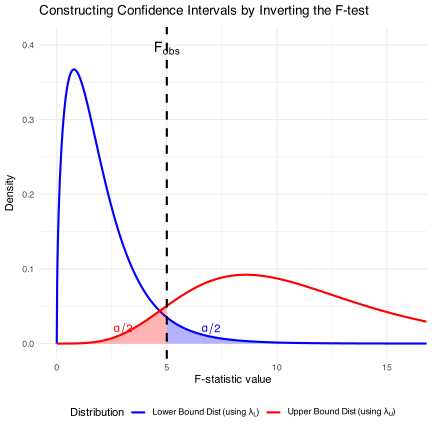
\includegraphics[keepaspectratio]{lec5-est_files/figure-pdf/fig-ci-inversion-1.pdf}}

}

\caption{\label{fig-ci-inversion}Illustration of constructing a
confidence interval for the non-centrality parameter \(\lambda\) by
inverting the F-test. The observed \(F_{obs}\) (dashed line) is the
\(97.5^{th}\) percentile of the distribution defined by the lower bound
\(\lambda_L\) (blue), and the \(2.5^{th}\) percentile of the
distribution defined by the upper bound \(\lambda_U\) (red). The shaded
areas each represent \(\alpha/2\).}

\end{figure}%

\textbf{3. The Interval for \(\rho^2\):}

Once \([\lambda_L, \lambda_U]\) are found numerically, we map them back
to the population \(R^2\) scale using the inverse relationship:

\[ \rho^2 = \frac{\lambda}{\lambda + (n-1)} \]

This produces an exact confidence interval \([\rho^2_L, \rho^2_U]\) for
the proportion of variance explained by the model in the population.

\section{\texorpdfstring{An Animation for Illustrating \(R^2_a\) Under
\(H_0\) and
\(H_1\)}{An Animation for Illustrating R\^{}2\_a Under H\_0 and H\_1}}\label{an-animation-for-illustrating-r2_a-under-h_0-and-h_1}

We simulate a dataset with \(n=30\) observations and consider a sequence
of nested models adding groups of predictors.

\textbf{Predictor Groups:}

\begin{enumerate}
\def\labelenumi{\arabic{enumi}.}
\tightlist
\item
  \textbf{Group 1 (\(k=1\)):} Add \(x_1\). (Signal under \(H_1\)).
\item
  \textbf{Group 2 (\(k=6\)):} Add \(x_2, \dots, x_6\) (Noise).
\item
  \textbf{Group 3 (\(k=11\)):} Add \(x_7, \dots, x_{11}\) (Noise).
\item
  \textbf{Group 4 (\(k=20\)):} Add \(x_{12}, \dots, x_{20}\) (Noise).
\end{enumerate}

\subsubsection{\texorpdfstring{Null Hypothesis
(\(H_0\))}{Null Hypothesis (H\_0)}}

Under \(H_0\), the true coefficient for \(x_1\) is \(\beta_1 = 0\). All
predictors are noise.

\begin{figure}[H]

{\centering \includegraphics[width=2.33in,height=\textheight,keepaspectratio]{figs/rss-h0-v6.png}

}

\caption{Simulation under H0: As predictors are added (pure noise),
standard R-squared increases while Adjusted R-squared and MSE remain
stable.}

\end{figure}%

\subsubsection{\texorpdfstring{Alternative Hypothesis
(\(H_1\))}{Alternative Hypothesis (H\_1)}}

Under \(H_1\), \(x_1\) is a true predictor (\(\beta_1 = 2\)). The
subsequent groups (\(x_2 \dots x_{20}\)) remain noise.

\begin{figure}[H]

{\centering \includegraphics[width=2.33in,height=\textheight,keepaspectratio]{figs/rss-h1-v6.png}

}

\caption{Simulation under H1: Adjusted R-squared correctly identifies
the signal at k=1, then penalizes the subsequent noise predictors.}

\end{figure}%

\section{A Data Example with House Price
Valuation}\label{a-data-example-with-house-price-valuation}

A real estate agency wants to refine their pricing model. They regress
the selling price of houses (\(y\)) on five predictors (\(X\)): Size,
Age, Bedrooms, Garage Capacity, and Lawn Size.

We assume the data has been collected and saved to
\texttt{house\_prices\_5pred.csv}.

\subsection{Visualize the Data}\label{visualize-the-data}

First, we load the dataset. We display the first 10 rows for PDF output,
or a full paged table for HTML.

\begin{longtable}[]{@{}rrrrrr@{}}
\caption{First 10 rows of House Prices}\tabularnewline
\toprule\noalign{}
Price & Size & Age & Beds & Garage & Lawn \\
\midrule\noalign{}
\endfirsthead
\toprule\noalign{}
Price & Size & Age & Beds & Garage & Lawn \\
\midrule\noalign{}
\endhead
\bottomrule\noalign{}
\endlastfoot
497808 & 3092 & 4 & 3 & 2 & 426 \\
364297 & 1802 & 26 & 5 & 0 & 88 \\
610217 & 2701 & 22 & 4 & 1 & 403 \\
536122 & 2745 & 38 & 4 & 0 & 437 \\
347259 & 2143 & 18 & 2 & 1 & 141 \\
343784 & 2754 & 49 & 5 & 1 & 186 \\
379522 & 2039 & 53 & 4 & 0 & 451 \\
341432 & 1758 & 43 & 5 & 1 & 832 \\
515913 & 3191 & 19 & 4 & 0 & 276 \\
292732 & 1298 & 17 & 2 & 2 & 804 \\
\end{longtable}

\subsection{Fit the Model}\label{fit-the-model}

We will solve for the coefficients \(\hat{\beta}\) using three distinct
methods.

\subsubsection*{Method 1: Naive Matrix
Formula}\label{method-1-naive-matrix-formula}
\addcontentsline{toc}{subsubsection}{Method 1: Naive Matrix Formula}

This method solves the normal equations directly on the raw data:
\(\hat{\beta} = (X^{\prime}X)^{-1}X^{\prime}y\).

\begin{verbatim}
Matrix X'X (Cross-products of predictors):
\end{verbatim}

\begin{verbatim}
          Intercept      Size     Age   Beds Garage     Lawn
Intercept        60    136483    1674    206     80    29392
Size         136483 343078981 3738402 469757 177877 63939128
Age            1674   3738402   63528   5874   2353   827130
Beds            206    469757    5874    776    281    98738
Garage           80    177877    2353    281    196    41915
Lawn          29392  63939128  827130  98738  41915 19306096
\end{verbatim}

\begin{verbatim}

Matrix X'y (Cross-products with response):
\end{verbatim}

\begin{verbatim}
                 [,1]
Intercept    25884407
Size      63115001244
Age         694594579
Beds         89683035
Garage       34067413
Lawn      12402228016
\end{verbatim}

\begin{verbatim}

Solved Coefficients (Beta):
\end{verbatim}

\begin{verbatim}
     Intercept     Size       Age     Beds   Garage    Lawn
[1,]    113186 129.3434 -1218.352 12664.16 875.1155 27.2443
\end{verbatim}

\subsubsection*{Method 2: Centralized
Formula}\label{method-2-centralized-formula}
\addcontentsline{toc}{subsubsection}{Method 2: Centralized Formula}

This method reduces multicollinearity issues. Formula:
\(\hat{\beta}_{\text{slope}} = (X_c^{\prime}X_c)^{-1}X_c^{\prime}y_c\).

\begin{verbatim}
Matrix X_c'X_c (Centered Sum of Squares):
\end{verbatim}

\begin{verbatim}
           Size    Age  Beds Garage     Lawn
Size   32618826 -69474  1165  -4100 -2919344
Age      -69474  16823   127    121     7093
Beds       1165    127    69      6    -2175
Garage    -4100    121     6     89     2726
Lawn   -2919344   7093 -2175   2726  4907935
\end{verbatim}

\begin{verbatim}

Matrix X_c'y_c (Centered Cross-products):
\end{verbatim}

\begin{verbatim}
             [,1]
Size   4235309234
Age     -27580376
Beds       813238
Garage    -445130
Lawn   -277680160
\end{verbatim}

\begin{verbatim}

Solved Coefficients (Beta):
\end{verbatim}

\begin{verbatim}
     Intercept     Size       Age     Beds   Garage    Lawn
[1,]    113186 129.3434 -1218.352 12664.16 875.1155 27.2443
\end{verbatim}

\subsubsection*{\texorpdfstring{Method 3: Using R's \texttt{lm}
Function}{Method 3: Using R's lm Function}}\label{method-3-using-rs-lm-function}
\addcontentsline{toc}{subsubsection}{Method 3: Using R's \texttt{lm}
Function}

This is the standard approach for practitioners.

\begin{verbatim}

Call:
lm(formula = Price ~ ., data = df)

Residuals:
    Min      1Q  Median      3Q     Max 
-135178  -36006    1710   26401  111967 

Coefficients:
              Estimate Std. Error t value Pr(>|t|)    
(Intercept) 113185.971  35675.435   3.173  0.00249 ** 
Size           129.343      8.927  14.490  < 2e-16 ***
Age          -1218.352    386.414  -3.153  0.00264 ** 
Beds         12664.157   6064.435   2.088  0.04150 *  
Garage         875.115   5316.490   0.165  0.86987    
Lawn            27.244     23.243   1.172  0.24629    
---
Signif. codes:  0 '***' 0.001 '**' 0.01 '*' 0.05 '.' 0.1 ' ' 1

Residual standard error: 49360 on 54 degrees of freedom
Multiple R-squared:  0.8161,    Adjusted R-squared:  0.799 
F-statistic: 47.92 on 5 and 54 DF,  p-value: < 2.2e-16
\end{verbatim}

\subsection{Visualization of Fitted Values vs
Mean}\label{visualization-of-fitted-values-vs-mean}

We define \(\hat{y}_0\) as the vector of the mean of \(y\)
(\(\bar{y}\)). We plot the actual \(y\) against our fitted model
\(\hat{y}\), using a green line to represent the ``Null Model''
(\(\hat{y}_0\)).

\emph{Note: Axes have been set so that X = Predicted Value and Y =
Actual Value.}

\pandocbounded{\includegraphics[keepaspectratio]{lec5-est_files/figure-pdf/plot-y-vs-yhat-1.pdf}}

\textbf{Question:}

\[ \bar y = \bar{\hat{y}} ?\]

\subsection{Computing Sums of Squares (SSE, SST,
SSR)}\label{computing-sums-of-squares-sse-sst-ssr}

We compare different methods to calculate the sources of variation.

\subsubsection{1. Naive Sum of Squared
Errors}\label{naive-sum-of-squared-errors}

This uses the standard summation definitions: \(\sum (Difference)^2\).

\begin{itemize}
\tightlist
\item
  \textbf{SST (Total):} Variation of \(y\) around \(\hat{y}_0\) (Mean).
\item
  \textbf{SSR (Regression):} Variation of \(\hat{y}\) around
  \(\hat{y}_0\) (Mean).
\item
  \textbf{SSE (Error):} Variation of \(y\) around \(\hat{y}\) (Model).
\end{itemize}

\begin{verbatim}
Naive Calculation:
\end{verbatim}

\begin{verbatim}
SST: 358921762209  SSR: 282617820807  SSE: 76303941402 
\end{verbatim}

\subsubsection{2. Pythagorean Shortcut (Vector
Lengths)}\label{pythagorean-shortcut-vector-lengths}

Based on the geometry of least squares, we can treat the variables as
vectors. Because the vectors are orthogonal, we can use squared lengths
(dot products with themselves).

Formula: \(SSR = ||\hat{y}||^2 - ||\hat{y}_0||^2\)

\begin{verbatim}
Pythagorean Calculation:
\end{verbatim}

\begin{verbatim}
SST: 358921762209  SSR: 282617820807  SSE: 76303941402 
\end{verbatim}

\subsubsection{Matrix Algebra Shortcuts}\label{matrix-algebra-shortcuts}

These formulas use the \(\beta\) and \(X\) matrices directly. This is
computationally efficient for large datasets.

\begin{itemize}
\tightlist
\item
  Formula A (Centered with \(y_c\)):
  \(SSR = \hat{\beta}_c^{\prime} X_c^{\prime} y_c\)
\item
  Formula B (Alternative with \(y\)):
  \(SSR = \hat{\beta}_c^{\prime} X_c^{\prime} y\)
\item
  Formula C (Uncentered):
  \(SSR = \hat{\beta}^{\prime} X^{\prime} y - n\bar{y}^2\)
\end{itemize}

\begin{longtable}[]{@{}
  >{\raggedright\arraybackslash}p{(\linewidth - 4\tabcolsep) * \real{0.3521}}
  >{\raggedright\arraybackslash}p{(\linewidth - 4\tabcolsep) * \real{0.4648}}
  >{\raggedleft\arraybackslash}p{(\linewidth - 4\tabcolsep) * \real{0.1831}}@{}}
\caption{Demonstration of SSR Formula Equivalence}\tabularnewline
\toprule\noalign{}
\begin{minipage}[b]{\linewidth}\raggedright
Metric
\end{minipage} & \begin{minipage}[b]{\linewidth}\raggedright
Formula
\end{minipage} & \begin{minipage}[b]{\linewidth}\raggedleft
Value
\end{minipage} \\
\midrule\noalign{}
\endfirsthead
\toprule\noalign{}
\begin{minipage}[b]{\linewidth}\raggedright
Metric
\end{minipage} & \begin{minipage}[b]{\linewidth}\raggedright
Formula
\end{minipage} & \begin{minipage}[b]{\linewidth}\raggedleft
Value
\end{minipage} \\
\midrule\noalign{}
\endhead
\bottomrule\noalign{}
\endlastfoot
SSR (Centered \(X_c,y_c\)) & \(\hat{\beta}_c' X_c' y_c\) &
282617820807 \\
SSR (Centered \(X_c\)) & \(\hat{\beta}_c' X_c' y\) & 282617820807 \\
SSR (Uncentered) & \(\hat{\beta}' X' y - n\bar{y}^2\) & 282617820807 \\
\end{longtable}

\subsection{Analysis of Variance
(ANOVA)}\label{analysis-of-variance-anova}

We now evaluate the sources of variation to test the overall model
significance.

\subsubsection*{1. Computing Sums of
Squares}\label{computing-sums-of-squares}
\addcontentsline{toc}{subsubsection}{1. Computing Sums of Squares}

We calculate the following components:

\begin{itemize}
\tightlist
\item
  Total Sum of Squares: \(\text{SST} = \sum (y_i - \bar{y})^2\)
\item
  Regression Sum of Squares:
  \(\text{SSR} = \sum (\hat{y}_i - \bar{y})^2\)
\item
  Sum of Squared Errors: \(\text{SSE} = \sum (y_i - \hat{y}_i)^2\)
\end{itemize}

\begin{verbatim}
SST: 715333529746  SSR: 583756306788  SSE: 131577222958 
\end{verbatim}

\subsubsection*{2. Manual ANOVA
Construction}\label{manual-anova-construction}
\addcontentsline{toc}{subsubsection}{2. Manual ANOVA Construction}

We build the table manually using the sums of squares and degrees of
freedom. We calculate the Mean Squares and the F-statistic:

\begin{itemize}
\tightlist
\item
  \(\text{MSR} = \text{SSR} / k\)
\item
  \(\text{MSE} = \text{SSE} / (n - k - 1)\)
\item
  \(\text{MST} = \text{SST} / (n - 1)\)
\item
  \(F = \text{MSR} / \text{MSE}\)
\end{itemize}

\begin{longtable}[]{@{}
  >{\raggedright\arraybackslash}p{(\linewidth - 10\tabcolsep) * \real{0.2794}}
  >{\raggedleft\arraybackslash}p{(\linewidth - 10\tabcolsep) * \real{0.0441}}
  >{\raggedleft\arraybackslash}p{(\linewidth - 10\tabcolsep) * \real{0.1912}}
  >{\raggedleft\arraybackslash}p{(\linewidth - 10\tabcolsep) * \real{0.1912}}
  >{\raggedleft\arraybackslash}p{(\linewidth - 10\tabcolsep) * \real{0.1765}}
  >{\raggedleft\arraybackslash}p{(\linewidth - 10\tabcolsep) * \real{0.1176}}@{}}
\caption{Manual ANOVA Table}\tabularnewline
\toprule\noalign{}
\begin{minipage}[b]{\linewidth}\raggedright
Source
\end{minipage} & \begin{minipage}[b]{\linewidth}\raggedleft
DF
\end{minipage} & \begin{minipage}[b]{\linewidth}\raggedleft
SS
\end{minipage} & \begin{minipage}[b]{\linewidth}\raggedleft
MS
\end{minipage} & \begin{minipage}[b]{\linewidth}\raggedleft
F\_Statistic
\end{minipage} & \begin{minipage}[b]{\linewidth}\raggedleft
P\_Value
\end{minipage} \\
\midrule\noalign{}
\endfirsthead
\toprule\noalign{}
\begin{minipage}[b]{\linewidth}\raggedright
Source
\end{minipage} & \begin{minipage}[b]{\linewidth}\raggedleft
DF
\end{minipage} & \begin{minipage}[b]{\linewidth}\raggedleft
SS
\end{minipage} & \begin{minipage}[b]{\linewidth}\raggedleft
MS
\end{minipage} & \begin{minipage}[b]{\linewidth}\raggedleft
F\_Statistic
\end{minipage} & \begin{minipage}[b]{\linewidth}\raggedleft
P\_Value
\end{minipage} \\
\midrule\noalign{}
\endhead
\bottomrule\noalign{}
\endlastfoot
Regression (Model) & 5 & 583756306788 & 116751261358 & 16.8591 & 0 \\
Error (Residual) & 19 & 131577222958 & 6925116998 & NA & NA \\
Total & 24 & 715333529746 & 29805563739 & NA & NA \\
\end{longtable}

\subsubsection*{\texorpdfstring{3. Standard R Output
(\texttt{anova})}{3. Standard R Output (anova)}}\label{standard-r-output-anova}
\addcontentsline{toc}{subsubsection}{3. Standard R Output
(\texttt{anova})}

We display the standard \texttt{summary()} which provides the
coefficients, t-tests, and the overall F-statistic found at the bottom.
We also show \texttt{anova()} which gives the sequential sum of squares.

\begin{verbatim}

ANOVA comparing intercept-only model to fitted model:
\end{verbatim}

\begin{verbatim}
Analysis of Variance Table

Model 1: Price ~ 1
Model 2: Price ~ Size + Age + Beds + Garage + Lawn
  Res.Df        RSS Df  Sum of Sq      F    Pr(>F)    
1     59 7.1533e+11                                   
2     54 1.3158e+11  5 5.8376e+11 47.915 < 2.2e-16 ***
---
Signif. codes:  0 '***' 0.001 '**' 0.01 '*' 0.05 '.' 0.1 ' ' 1
\end{verbatim}

\begin{verbatim}
Analysis of Variance Table

Response: Price
          Df     Sum Sq    Mean Sq  F value    Pr(>F)    
Size       1 5.4992e+11 5.4992e+11 225.6914 < 2.2e-16 ***
Age        1 2.0657e+10 2.0657e+10   8.4777  0.005216 ** 
Beds       1 9.5872e+09 9.5872e+09   3.9346  0.052396 .  
Garage     1 2.4151e+08 2.4151e+08   0.0991  0.754107    
Lawn       1 3.3476e+09 3.3476e+09   1.3739  0.246291    
Residuals 54 1.3158e+11 2.4366e+09                       
---
Signif. codes:  0 '***' 0.001 '**' 0.01 '*' 0.05 '.' 0.1 ' ' 1
\end{verbatim}

\subsection{Coefficient of Determination and Variance
Decomposition}\label{coefficient-of-determination-and-variance-decomposition}

We calculate \(R^2\) and Adjusted \(R^2\), and then present them in a
\textbf{Variance Decomposition Table}.

\subsubsection*{1. Calculation}\label{calculation}
\addcontentsline{toc}{subsubsection}{1. Calculation}

We calculate the coefficients of determination:

\begin{itemize}
\tightlist
\item
  Standard \(R^2 = 1 - \frac{\text{SSE}}{\text{SST}}\)
\item
  Adjusted \(R^2_a = 1 - \frac{\text{MSE}}{\text{MST}}\)
\end{itemize}

\begin{verbatim}
Standard R^2:   0.8161 
\end{verbatim}

\begin{verbatim}
Adjusted R^2:   0.7677 
\end{verbatim}

\subsubsection*{2. Variance Decomposition
Table}\label{variance-decomposition-table}
\addcontentsline{toc}{subsubsection}{2. Variance Decomposition Table}

This table extends standard ANOVA. While ANOVA focuses on \textbf{Mean
Squares (MS)} for hypothesis testing (is \(MSR > MSE\)?), this table
focuses on \textbf{Variance Components (\(\hat{\sigma}^2\))} for
estimation (how much variance is Signal vs.~Noise?). We estimate the
variance components as follows:

\begin{itemize}
\item
  Signal Variance: \(\hat{\sigma}^2_\mu = \text{MST} - \text{MSE}\)
\item
  Noise Variance: \(\hat{\sigma}^2 = \text{MSE}\)
\item
  Total Variance: \(\hat{\sigma}^2_Y = \text{MST}\)
\item
  \textbf{Signal Variance (\(\hat{\sigma}^2_\mu\)):} Estimated by
  \(MST - MSE\). (Note: \(MSR\) is biased and overestimates signal).
\item
  \textbf{Noise Variance (\(\hat{\sigma}^2\)):} Estimated by \(MSE\).
\item
  \textbf{Total Variance (\(\hat{\sigma}^2_Y\)):} Estimated by \(MST\).
\end{itemize}

\begin{longtable}[]{@{}
  >{\raggedright\arraybackslash}p{(\linewidth - 10\tabcolsep) * \real{0.1899}}
  >{\raggedleft\arraybackslash}p{(\linewidth - 10\tabcolsep) * \real{0.0380}}
  >{\raggedleft\arraybackslash}p{(\linewidth - 10\tabcolsep) * \real{0.1646}}
  >{\raggedleft\arraybackslash}p{(\linewidth - 10\tabcolsep) * \real{0.1519}}
  >{\raggedleft\arraybackslash}p{(\linewidth - 10\tabcolsep) * \real{0.3165}}
  >{\raggedleft\arraybackslash}p{(\linewidth - 10\tabcolsep) * \real{0.1392}}@{}}
\caption{Variance Decomposition Table: Estimating Signal
vs.~Noise}\tabularnewline
\toprule\noalign{}
\begin{minipage}[b]{\linewidth}\raggedright
Component
\end{minipage} & \begin{minipage}[b]{\linewidth}\raggedleft
DF
\end{minipage} & \begin{minipage}[b]{\linewidth}\raggedleft
SS
\end{minipage} & \begin{minipage}[b]{\linewidth}\raggedleft
MS
\end{minipage} & \begin{minipage}[b]{\linewidth}\raggedleft
Value (\(\hat{\sigma}^2\))
\end{minipage} & \begin{minipage}[b]{\linewidth}\raggedleft
Proportion
\end{minipage} \\
\midrule\noalign{}
\endfirsthead
\toprule\noalign{}
\begin{minipage}[b]{\linewidth}\raggedright
Component
\end{minipage} & \begin{minipage}[b]{\linewidth}\raggedleft
DF
\end{minipage} & \begin{minipage}[b]{\linewidth}\raggedleft
SS
\end{minipage} & \begin{minipage}[b]{\linewidth}\raggedleft
MS
\end{minipage} & \begin{minipage}[b]{\linewidth}\raggedleft
Value (\(\hat{\sigma}^2\))
\end{minipage} & \begin{minipage}[b]{\linewidth}\raggedleft
Proportion
\end{minipage} \\
\midrule\noalign{}
\endhead
\bottomrule\noalign{}
\endlastfoot
Signal (Model) & 5 & 583756306788 & NA & 22880446742 & 0.7677 \\
Noise (Error) & 19 & 131577222958 & 6925116998 & 6925116998 & 0.2323 \\
Total (Y) & 24 & 715333529746 & 29805563739 & 29805563739 & 1.0000 \\
\end{longtable}

\subsection{\texorpdfstring{Confidence Interval for Population \(R^2\)
(\(\rho^2\))}{Confidence Interval for Population R\^{}2 (\textbackslash rho\^{}2)}}\label{confidence-interval-for-population-r2-rho2}

We construct a 95\% confidence interval for the population proportion of
variance explained (\(\rho^2\)).

\subsubsection*{1. Manual Inversion
Method}\label{manual-inversion-method}
\addcontentsline{toc}{subsubsection}{1. Manual Inversion Method}

We solve for the non-centrality parameters \(\lambda_L\) and
\(\lambda_U\) such that our observed \(F_{obs}\) corresponds to the
appropriate quantiles.

\begin{verbatim}
Manual Calculation:
\end{verbatim}

\begin{verbatim}
95% CI for Population Rho^2: [ 0.53 ,  0.8616 ]
\end{verbatim}

\subsubsection*{\texorpdfstring{2. Using R Package
\texttt{MBESS}}{2. Using R Package MBESS}}\label{using-r-package-mbess}
\addcontentsline{toc}{subsubsection}{2. Using R Package \texttt{MBESS}}

The \texttt{MBESS} package automates this procedure. We use
\texttt{Random.Predictors\ =\ FALSE} to match the fixed-predictor
assumption used in our manual calculation.

\begin{verbatim}
$Lower.Conf.Limit.R2
[1] 0.5300075

$Prob.Less.Lower
[1] 0.025

$Upper.Conf.Limit.R2
[1] 0.8615512

$Prob.Greater.Upper
[1] 0.025
\end{verbatim}

\section{Underfitting and
Overfitting}\label{underfitting-and-overfitting}

We compare the properties of two competing estimators for the mean
response vector \(\mu = E[y]\).

\subsection{Notation and Setup}\label{notation-and-setup}

We consider the general linear model: \[
y = X\beta + e = X_1\beta_1 + X_2\beta_2 + e
\] where \(X_1\) is \(n \times p_1\), \(X_2\) is \(n \times p_2\), and
\(\text{Var}(e) = \sigma^2 I\).

We distinguish between two estimation approaches based on this model:

\textbf{1. Full Model (\(M_1\))} We estimate \(\beta\) without
restrictions. The estimator projects \(y\) onto the full column space
\(\text{Col}(X)\). \[
\begin{aligned}
P_1 &= X(X^T X)^{-1}X^T & (\text{Projection onto } \text{Col}(X)) \\
\hat{y}_1 &= P_1 y & (\text{Unrestricted Estimator})
\end{aligned}
\]

\textbf{2. Reduced Model (\(M_0\))} We estimate \(\beta\) subject to the
constraint: \[
M_0: \beta_2 = 0
\] This effectively reduces the model to \(y = X_1\beta_1 + e\),
projecting \(y\) onto the subspace \(\text{Col}(X_1)\). \[
\begin{aligned}
P_0 &= X_1(X_1^T X_1)^{-1}X_1^T & (\text{Projection onto } \text{Col}(X_1)) \\
\hat{y}_0 &= P_0 y & (\text{Restricted Estimator})
\end{aligned}
\]

\textbf{Key Geometric Property:} Since the constraint \(\beta_2=0\)
restricts the estimation to a subspace
(\(\text{Col}(X_1) \subset \text{Col}(X)\)), we have the nesting
property: \[
P_1 P_0 = P_0 \quad \text{and} \quad P_1 - P_0 \text{ is a projection matrix.}
\]

\subsection{Case 1: Underfitting}\label{case-1-underfitting}

\textbf{The Truth:} The Full Model (\(M_1\)) is correct. \[
y = X_1\beta_1 + X_2\beta_2 + e, \quad \beta_2 \neq 0
\] The true mean is \(\mu = X_1\beta_1 + X_2\beta_2\).

We analyze the properties of the \textbf{Reduced Estimator}
\(\hat{y}_0\) (from \(M_0\)) compared to the correct Full Estimator
\(\hat{y}_1\) (from \(M_1\)).

\begin{theorem}[Bias-Variance Tradeoff in
Underfitting]\protect\hypertarget{thm-underfitting}{}\label{thm-underfitting}

When \(M_1\) is true:

\begin{enumerate}
\def\labelenumi{\arabic{enumi}.}
\tightlist
\item
  \textbf{Bias:} The estimator \(\hat{y}_0\) is \textbf{biased}, while
  \(\hat{y}_1\) is unbiased.
  \[ \text{Bias}(\hat{y}_0) = -(I - P_0) X_2 \beta_2 \]
\item
  \textbf{Variance:} The estimator \(\hat{y}_0\) has \textbf{smaller
  variance} (matrix difference is positive semidefinite).
  \[ \text{Var}(\hat{y}_1) - \text{Var}(\hat{y}_0) = \sigma^2 (P_1 - P_0) \ge 0 \]
\end{enumerate}

\end{theorem}

\begin{proof}
\textbf{Part 1 (Bias):} \[
\begin{aligned}
E[\hat{y}_0] &= P_0 E[y] = P_0(X_1\beta_1 + X_2\beta_2) \\
&= X_1\beta_1 + P_0 X_2 \beta_2 \quad (\text{Since } P_0 X_1 = X_1)
\end{aligned}
\] The bias is: \[
\text{Bias} = E[\hat{y}_0] - \mu = (X_1\beta_1 + P_0 X_2 \beta_2) - (X_1\beta_1 + X_2\beta_2) = -(I - P_0)X_2\beta_2
\]

\textbf{Part 2 (Variance):} \[
\text{Var}(\hat{y}_1) = \sigma^2 P_1, \quad \text{Var}(\hat{y}_0) = \sigma^2 P_0
\] The difference is \(\sigma^2(P_1 - P_0)\). Since
\(\text{Col}(X_1) \subset \text{Col}(X)\), the difference \(P_1 - P_0\)
projects onto the orthogonal complement of \(\text{Col}(X_1)\) within
\(\text{Col}(X)\). It is idempotent and positive semidefinite.
\end{proof}

\textbf{Remark: Scalar Variance and Coefficients}

From the matrix inequality above, we can state that for any arbitrary
vector \(a\), the scalar variance of the linear combination
\(a^T \hat{y}\) is always smaller in the reduced model: \[
\text{Var}(a^T \hat{y}_0) \le \text{Var}(a^T \hat{y}_1)
\]

We can extend this property to the regression coefficients
\(\hat{\beta}\). Since \(\hat{y} = X\hat{\beta}\), we can recover the
coefficients from the fitted values using the left pseudo-inverse:

\[
\begin{aligned}
(X^T X)^{-1}X^T (X\hat{\beta}) &= (X^T X)^{-1}X^T \hat{y} \\
\underbrace{(X^T X)^{-1}(X^T X)}_{I} \hat{\beta} &= (X^T X)^{-1}X^T \hat{y}
\end{aligned}
\]

\begin{corollary}[Variance of
Coefficients]\protect\hypertarget{cor-beta-variance}{}\label{cor-beta-variance}

Because \(\hat{\beta}\) is a linear transformation of \(\hat{y}\), the
variance reduction in \(\hat{y}_0\) propagates to the coefficients.

For any specific coefficient \(\beta_j\) included in the reduced model
(i.e., \(\beta_j \in \beta_1\)), the variance of the estimator is
smaller in the reduced model than in the full model:
\[ \text{Var}(\hat{\beta}_{j, reduced}) \le \text{Var}(\hat{\beta}_{j, full}) \]

\end{corollary}

\textbf{Conclusion:} Using \(M_0\) when \(M_1\) is true introduces bias
but reduces variance for both the fitted values and the estimated
coefficients.

\subsection{Case 2: Overfitting}\label{case-2-overfitting}

\textbf{The Truth:} The Reduced Model (\(M_0\)) is correct. \[
y = X_1\beta_1 + e \quad (\text{i.e., } \beta_2 = 0)
\] The true mean is \(\mu = X_1\beta_1\).

We analyze the properties of the \textbf{Full Estimator} \(\hat{y}_1\)
(from \(M_1\)) compared to the correct Reduced Estimator \(\hat{y}_0\)
(from \(M_0\)).

\begin{theorem}[Variance Inflation in
Overfitting]\protect\hypertarget{thm-overfitting}{}\label{thm-overfitting}

When \(M_0\) is true:

\begin{enumerate}
\def\labelenumi{\arabic{enumi}.}
\tightlist
\item
  \textbf{Bias:} Both estimators are \textbf{unbiased}.
  \[ E[\hat{y}_1] = \mu \quad \text{and} \quad E[\hat{y}_0] = \mu \]
\item
  \textbf{Variance:} The estimator \(\hat{y}_1\) has
  \textbf{unnecessarily higher variance}.
  \[ \text{Var}(\hat{y}_1) \ge \text{Var}(\hat{y}_0) \]
\end{enumerate}

\end{theorem}

\begin{proof}
\textbf{Part 1 (Bias):} Since \(\mu = X_1\beta_1\): \[
E[\hat{y}_1] = P_1 X_1\beta_1 = X_1\beta_1 = \mu \quad (\text{Since } X_1 \in \text{Col}(X))
\] \[
E[\hat{y}_0] = P_0 X_1\beta_1 = X_1\beta_1 = \mu \quad (\text{Since } X_1 \in \text{Col}(X_1))
\]

\textbf{Part 2 (Variance):} As shown in Case 1, the difference is
\(\sigma^2(P_1 - P_0)\). The cost of overfitting is purely variance
inflation. The total variance (trace) increases by the number of
unnecessary parameters (\(p_2\)): \[
\text{tr}(\text{Var}(\hat{y}_1)) - \text{tr}(\text{Var}(\hat{y}_0)) = \sigma^2 (\text{tr}(P_1) - \text{tr}(P_0)) = \sigma^2 (p_{full} - p_{reduced}) = \sigma^2 p_2
\]
\end{proof}

\textbf{Conclusion:} Using \(M_1\) when \(M_0\) is true offers no
benefit in bias but strictly increases estimation variance.

\bookmarksetup{startatroot}

\chapter{Generalized Inverses}\label{generalized-inverses}

\section{Motivation}\label{motivation-1}

Consider the linear system \(X\beta = y\). In \(\mathbb{R}^2\), if
\(X = [x_1, x_2]\) is invertible, the solution is unique:
\(\beta = X^{-1}y\). This satisfies \(X(X^{-1}y) = y\).However, if \(X\)
is not square or not invertible (e.g., \(X\) is \(2 \times 3\)),
\(X\beta = y\) does not have a unique solution. We seek a matrix \(G\)
such that \(\beta = Gy\) provides a solution whenever \(y \in C(X)\)
(the column space of X). Substituting \(\beta = Gy\) into the equation
\(X\beta = y\): \[
X(Gy) = y \quad \forall y \in C(X)
\] Since any \(y \in C(X)\) can be written as \(Xw\) for some vector
\(w\): \[
XGXw = Xw \quad \forall w
\] This implies the defining condition: \[
XGX = X
\]

\section{Definition of Generalized
Inverse}\label{definition-of-generalized-inverse}

\begin{definition}[Generalized
Inverse]\protect\hypertarget{def-gen-inverse}{}\label{def-gen-inverse}

Let \(X\) be an \(n \times p\) matrix. A matrix \(X^-\) of size
\(p \times n\) is called a \textbf{generalized inverse} of \(X\) if it
satisfies: \[
XX^-X = X
\]

\end{definition}

\begin{example}[Examples of Generalized
Inverse]\protect\hypertarget{exm-ginverse}{}\label{exm-ginverse}

~

\begin{itemize}
\item
  \textbf{Example 1: Diagonal Matrix} If
  \(X = \text{diag}(\lambda_1, \lambda_2, 0, 0)\), we can write it in
  matrix form as: \[
    X = \begin{pmatrix}
    \lambda_1 & 0 & 0 & 0 \\
    0 & \lambda_2 & 0 & 0 \\
    0 & 0 & 0 & 0 \\
    0 & 0 & 0 & 0
    \end{pmatrix}
    \] A generalized inverse is obtained by inverting the non-zero
  elements: \[
    X^- = \begin{pmatrix}
    \lambda_1^{-1} & 0 & 0 & 0 \\
    0 & \lambda_2^{-1} & 0 & 0 \\
    0 & 0 & 0 & 0 \\
    0 & 0 & 0 & 0
    \end{pmatrix}
    \]
\item
  \textbf{Example 2: Row Vector} Let \(X = (1, 2, 3)\). One possible
  generalized inverse is a column vector where the first element is the
  reciprocal of the first non-zero element of \(X\) (which is \(1\)),
  and others are zero: \[
    X^- = \begin{pmatrix} 1 \\ 0 \\ 0 \end{pmatrix}
    \] \textbf{Verification:} \[
    XX^-X = (1, 2, 3) \begin{pmatrix} 1 \\ 0 \\ 0 \end{pmatrix} (1, 2, 3) = (1) \cdot (1, 2, 3) = (1, 2, 3) = X
    \] Other valid generalized inverses include
  \(\begin{pmatrix} 0 \\ 1/2 \\ 0 \end{pmatrix}\) or
  \(\begin{pmatrix} 0 \\ 0 \\ 1/3 \end{pmatrix}\).
\item
  \textbf{Example 3: Rank Deficient Matrix} Let
  \(A = \begin{pmatrix} 2 & 2 & 3 \\ 1 & 0 & 1 \\ 3 & 2 & 4 \end{pmatrix}\).
  Note that Row 3 = Row 1 + Row 2, so Rank\((A) = 2\).

  \textbf{Solution:} A generalized inverse can be found by locating a
  non-singular \(2 \times 2\) submatrix, inverting it, and padding the
  rest with zeros. Let's take the top-left minor
  \(M = \begin{pmatrix} 2 & 2 \\ 1 & 0 \end{pmatrix}\). The inverse is
  \(M^{-1} = \frac{1}{-2}\begin{pmatrix} 0 & -2 \\ -1 & 2 \end{pmatrix} = \begin{pmatrix} 0 & 1 \\ 0.5 & -1 \end{pmatrix}\).

  Placing this in the corresponding position in \(A^-\) and setting the
  rest to 0: \[
    A^- = \begin{pmatrix} 0 & 1 & 0 \\ 0.5 & -1 & 0 \\ 0 & 0 & 0 \end{pmatrix}
    \]

  \textbf{Verification (\(AA^-A = A\)):} First, compute \(AA^-\): \[
    AA^- = \begin{pmatrix} 2 & 2 & 3 \\ 1 & 0 & 1 \\ 3 & 2 & 4 \end{pmatrix} \begin{pmatrix} 0 & 1 & 0 \\ 0.5 & -1 & 0 \\ 0 & 0 & 0 \end{pmatrix} = \begin{pmatrix} 1 & 0 & 0 \\ 0 & 1 & 0 \\ 1 & 1 & 0 \end{pmatrix}
    \] Then multiply by \(A\): \[
    (AA^-)A = \begin{pmatrix} 1 & 0 & 0 \\ 0 & 1 & 0 \\ 1 & 1 & 0 \end{pmatrix} \begin{pmatrix} 2 & 2 & 3 \\ 1 & 0 & 1 \\ 3 & 2 & 4 \end{pmatrix} = \begin{pmatrix} 2 & 2 & 3 \\ 1 & 0 & 1 \\ 3 & 2 & 4 \end{pmatrix} = A
    \]
\end{itemize}

\end{example}

\section{A Procedure to Find a Generalized
Inverse}\label{a-procedure-to-find-a-generalized-inverse}

If we can partition \(X\) (possibly after permuting rows/columns) such
that \(R_{11}\) is a non-singular rank \(r\) submatrix:

\[
X = \begin{pmatrix} R_{11} & R_{12} \\ R_{21} & R_{22} \end{pmatrix}
\]

Then a generalized inverse is:

\[
X^- = \begin{pmatrix} R_{11}^{-1} & 0 \\ 0 & 0 \end{pmatrix}
\]

\textbf{Verification:}

\[
\begin{aligned}
XX^-X &= \begin{pmatrix} R_{11} & R_{12} \\ R_{21} & R_{22} \end{pmatrix} \begin{pmatrix} R_{11}^{-1} & 0 \\ 0 & 0 \end{pmatrix} \begin{pmatrix} R_{11} & R_{12} \\ R_{21} & R_{22} \end{pmatrix} \\
&= \begin{pmatrix} I_r & 0 \\ R_{21}R_{11}^{-1} & 0 \end{pmatrix} \begin{pmatrix} R_{11} & R_{12} \\ R_{21} & R_{22} \end{pmatrix} \\
&= \begin{pmatrix} R_{11} & R_{12} \\ R_{21} & R_{21}R_{11}^{-1}R_{12} \end{pmatrix}
\end{aligned}
\] Note that since rank\((X) = \text{rank}(R_{11})\), the rows of
\([R_{21}, R_{22}]\) are linear combinations of \([R_{11}, R_{12}]\),
implying \(R_{22} = R_{21}R_{11}^{-1}R_{12}\). Thus, \(XX^-X = X\).

\textbf{An Algorithm for Finding a Generalized Inverse}

A systematic procedure to find a generalized inverse \(A^-\) for any
matrix \(A\):

\begin{enumerate}
\def\labelenumi{\arabic{enumi}.}
\tightlist
\item
  Find any non-singular \(r \times r\) submatrix \(C\), where \(r\) is
  the rank of \(A\). It is not necessary for the elements of \(C\) to
  occupy adjacent rows and columns in \(A\).
\item
  Find \(C^{-1}\) and \((C^{-1})'\).
\item
  Replace the elements of \(C\) in \(A\) with the elements of
  \((C^{-1})'\).
\item
  Replace all other elements in \(A\) with zeros.
\item
  Transpose the resulting matrix.
\end{enumerate}

\textbf{Matrix Visual Representation} \[
\underset{\text{Original } A}{\begin{pmatrix}
\times & \otimes & \times & \otimes \\
\times & \otimes & \times & \otimes \\
\times & \times & \times & \times
\end{pmatrix}}
\xrightarrow[\text{with } (C^{-1})']{\text{Replace } C}
\underset{\text{Intermediate}}{\begin{pmatrix}
\times & \triangle & \times & \triangle \\
\times & \triangle & \times & \triangle \\
\times & \times & \times & \times
\end{pmatrix}}
\xrightarrow[\text{Result}]{\text{Transpose}}
\underset{\text{Final } A^-}{\begin{pmatrix}
\times & \times & \times \\
\square & \square & \times \\
\times & \times & \times \\
\square & \square & \times
\end{pmatrix}}
\]

\textbf{Legend:}

\begin{itemize}
\tightlist
\item
  \(\otimes\): Elements of submatrix \(C\)
\item
  \(\triangle\): Elements of \((C^{-1})'\)
\item
  \(\square\): Elements of \(C^{-1}\) (after transposition)
\item
  \(\times\): Other elements (replaced by 0 in the final calculation)
\end{itemize}

\section{Moore-Penrose Inverse}\label{moore-penrose-inverse}

The Moore-Penrose inverse (denoted \(X^+\)) is a unique generalized
inverse defined via Singular Value Decomposition (SVD).

If \(X\) has SVD: \[
X = U \begin{pmatrix} \Lambda_r & 0 \\ 0 & 0 \end{pmatrix} V'
\]

Then the Moore-Penrose inverse is: \[
X^+ = V \begin{pmatrix} \Lambda_r^{-1} & 0 \\ 0 & 0 \end{pmatrix} U'
\]

where \(\Lambda_r = \text{diag}(\lambda_1, \dots, \lambda_r)\) contains
the singular values. Unlike standard generalized inverses, \(X^+\) is
unique.

\textbf{Verification:}

We verify that \(X^+\) satisfies the condition \(XX^+X = X\).

\begin{enumerate}
\def\labelenumi{\arabic{enumi}.}
\item
  \textbf{Substitute definitions:} \[
  XX^+X = \left[ U \begin{pmatrix} \Lambda_r & 0 \\ 0 & 0 \end{pmatrix} V' \right] \left[ V \begin{pmatrix} \Lambda_r^{-1} & 0 \\ 0 & 0 \end{pmatrix} U' \right] \left[ U \begin{pmatrix} \Lambda_r & 0 \\ 0 & 0 \end{pmatrix} V' \right]
  \]
\item
  \textbf{Apply orthogonality:} Recall that \(V'V = I\) and \(U'U = I\).
  \[
  = U \begin{pmatrix} \Lambda_r & 0 \\ 0 & 0 \end{pmatrix} \underbrace{(V'V)}_{I} \begin{pmatrix} \Lambda_r^{-1} & 0 \\ 0 & 0 \end{pmatrix} \underbrace{(U'U)}_{I} \begin{pmatrix} \Lambda_r & 0 \\ 0 & 0 \end{pmatrix} V'
  \]
\item
  \textbf{Multiply diagonal matrices:} \[
  = U \left[ \begin{pmatrix} \Lambda_r & 0 \\ 0 & 0 \end{pmatrix} \begin{pmatrix} \Lambda_r^{-1} & 0 \\ 0 & 0 \end{pmatrix} \begin{pmatrix} \Lambda_r & 0 \\ 0 & 0 \end{pmatrix} \right] V'
  \] Since
  \(\Lambda_r \Lambda_r^{-1} \Lambda_r = I \cdot \Lambda_r = \Lambda_r\):
  \[
  = U \begin{pmatrix} \Lambda_r & 0 \\ 0 & 0 \end{pmatrix} V' = X
  \]
\end{enumerate}

\section{Solving Linear Systems with Generalized
Inverse}\label{solving-linear-systems-with-generalized-inverse}

We apply generalized inverses to solve systems of linear equations
\(X\beta = c\) where \(X\) is \(n \times p\).

\begin{definition}[Consistency and
Solution]\protect\hypertarget{def-consistency}{}\label{def-consistency}

The system \(X\beta = c\) is consistent if and only if
\(c \in \text{Col}(X)\) (the column space of \(X\)). If consistent,
\(\beta = X^- c\) is a solution.

\end{definition}

\textbf{Proof:} If the system is consistent, there exists some \(b\)
such that \(Xb = c\). Using the definition \(XX^-X = X\): \[
X(X^- c) = X(X^- X b) = (XX^-X)b = Xb = c
\] Thus, \(X^-c\) is a solution. Note that the solution is not unique if
\(X\) is not full rank.

\begin{example}[Examples of Solutions of Linear System with Generalized
Inverse]\protect\hypertarget{exm-gi-sol-ls}{}\label{exm-gi-sol-ls}

~

\begin{itemize}
\item
  \textbf{Example 1: Underdetermined System}

  Let \(X = \begin{pmatrix} 1 & 2 & 3 \end{pmatrix}\) and we want to
  solve \(X\beta = 4\).

  \textbf{Solution 1:} Using the generalized inverse
  \(X^- = \begin{pmatrix} 1 \\ 0 \\ 0 \end{pmatrix}\): \[
  \beta = X^- \cdot 4 = \begin{pmatrix} 1 \\ 0 \\ 0 \end{pmatrix} 4 = \begin{pmatrix} 4 \\ 0 \\ 0 \end{pmatrix}
  \] \textbf{Verification:} \[
  X\beta = \begin{pmatrix} 1 & 2 & 3 \end{pmatrix} \begin{pmatrix} 4 \\ 0 \\ 0 \end{pmatrix} = 1(4) + 2(0) + 3(0) = 4 \quad \checkmark
  \]

  \textbf{Solution 2:} Using another generalized inverse
  \(X^- = \begin{pmatrix} 0 \\ 0 \\ 1/3 \end{pmatrix}\): \[
  \beta = X^- \cdot 4 = \begin{pmatrix} 0 \\ 0 \\ 1/3 \end{pmatrix} 4 = \begin{pmatrix} 0 \\ 0 \\ 4/3 \end{pmatrix}
  \] \textbf{Verification:} \[
  X\beta = \begin{pmatrix} 1 & 2 & 3 \end{pmatrix} \begin{pmatrix} 0 \\ 0 \\ 4/3 \end{pmatrix} = 0 + 0 + 3(4/3) = 4 \quad \checkmark
  \]
\item
  \textbf{Example 2: Overdetermined System}

  Let \(X = \begin{pmatrix} 1 \\ 2 \\ 3 \end{pmatrix}\). Solve
  \(X\beta = \begin{pmatrix} 2 \\ 4 \\ 6 \end{pmatrix} = c\). Here
  \(c = 2X\), so the system is consistent. Since \(X\) is a column
  vector, \(\beta\) is a scalar.

  \textbf{Solution:} Using the generalized inverse
  \(X^- = \begin{pmatrix} 1 & 0 & 0 \end{pmatrix}\): \[
  \beta = X^- c = \begin{pmatrix} 1 & 0 & 0 \end{pmatrix} \begin{pmatrix} 2 \\ 4 \\ 6 \end{pmatrix} = 1(2) + 0(4) + 0(6) = 2
  \] \textbf{Verification:} \[
  X\beta = \begin{pmatrix} 1 \\ 2 \\ 3 \end{pmatrix} (2) = \begin{pmatrix} 2 \\ 4 \\ 6 \end{pmatrix} = c \quad \checkmark
  \]
\end{itemize}

\end{example}

\section{\texorpdfstring{Least Squares for Non-full-rank \(X\) with
Generalized
Inverse}{Least Squares for Non-full-rank X with Generalized Inverse}}\label{least-squares-for-non-full-rank-x-with-generalized-inverse}

\subsection{\texorpdfstring{Projection Matrix with Generalized Inverse
of
\(X'X\)}{Projection Matrix with Generalized Inverse of X\textquotesingle X}}\label{projection-matrix-with-generalized-inverse-of-xx}

For the normal equations \((X'X)\beta = X'y\), a solution is given by:
\[
\hat{\beta} = (X'X)^- X'y
\] The fitted values are \[\hat{y} = X\hat{\beta} = X(X'X)^- X'y.\] This
\(\hat{y}\) represents the unique orthogonal projection of \(y\) onto
\(\text{Col}(X)\).

\subsection{Invariance and Uniqueness of ``the'' Projection
Matrix}\label{invariance-and-uniqueness-of-the-projection-matrix}

\begin{theorem}[Transpose Property of Generalized
Inverses]\protect\hypertarget{thm-transpose}{}\label{thm-transpose}

\((X^-)'\) is a version of \((X')^-\). That is, \((X^-)'\) is a
generalized inverse of \(X'\).

\end{theorem}

\begin{proof}
By definition, a generalized inverse \(X^-\) satisfies the property: \[
X X^- X = X
\]

To verify that \((X^-)'\) is a generalized inverse of \(X'\), we need to
show that it satisfies the condition \(A G A = A\) where \(A = X'\) and
\(G = (X^-)'\).

\begin{enumerate}
\def\labelenumi{\arabic{enumi}.}
\item
  Start with the fundamental definition: \[
  X X^- X = X
  \]
\item
  Take the transpose of both sides of the equation: \[
  (X X^- X)' = X'
  \]
\item
  Apply the reverse order law for transposes, \((ABC)' = C' B' A'\): \[
  X' (X^-)' X' = X'
  \]
\end{enumerate}

Since substituting \((X^-)'\) into the generalized inverse equation for
\(X'\) yields \(X'\), \((X^-)'\) is a valid generalized inverse of
\(X'\).
\end{proof}

\begin{lemma}[Invariance of Generalized Least
Squares]\protect\hypertarget{lem-invariance}{}\label{lem-invariance}

For any version of the generalized inverse \((X'X)^-\), the matrix
\(X'(X'X)^- X'\) is invariant and equals \(X'\). \[
X'X(X'X)^- X' = X'
\]

\end{lemma}

\textbf{Proof (using Projection):} Let \(P = X(X'X)^- X'\). This is the
projection matrix onto \(\text{Col}(X)\). By definition of projection,
\(Px = x\) for any \(x \in \text{Col}(X)\). Since columns of \(X\) are
in \(\text{Col}(X)\), \(PX = X\). Taking the transpose:
\((PX)' = X' \implies X'P' = X'\). Since projection matrices are
symmetric (\(P=P'\)), \(X'P = X'\). Substituting \(P\):
\(X' X (X'X)^- X' = X'\).

\textbf{Proof (Direct Matrix Manipulation):} Decompose
\(y = X\beta + e\) where \(e \perp \text{Col}(X)\) (i.e., \(X'e = 0\)).
\[
\begin{aligned}
X'X(X'X)^- X' y &= X'X(X'X)^- X' (X\beta + e) \\
&= X'X(X'X)^- X'X\beta + X'X(X'X)^- X'e
\end{aligned}
\] Using the property \(A A^- A = A\) (where \(A=X'X\)), the first term
becomes \(X'X\beta\). The second term is 0 because \(X'e = 0\). Thus,
the expression simplifies to
\(X'X\beta = X'(X\beta) = X'\hat{y}_{\text{proj}}\). This implies the
operator acts as \(X'\).

\begin{theorem}[Properties of Projection Matrix
\(P\)]\protect\hypertarget{thm-proj-properties}{}\label{thm-proj-properties}

Let \(P = X(X'X)^- X'\). This matrix has the following properties:

\begin{enumerate}
\def\labelenumi{\arabic{enumi}.}
\item
  \textbf{Symmetry:} \(P = P'\).
\item
  \textbf{Idempotence:} \(P^2 = P\). \[
  P^2 = X(X'X)^- X' X(X'X)^- X' = X(X'X)^- (X'X (X'X)^- X')
  \] Using the identity from Lemma~\ref{lem-invariance}
  (\(X'X(X'X)^- X' = X'\)), this simplifies to: \[
  X(X'X)^- X' = P
  \]
\item
  \textbf{Uniqueness:} \(P\) is unique and invariant to the choice of
  the generalized inverse \((X'X)^-\).
\end{enumerate}

\end{theorem}

\begin{proof}
\textbf{Proof of Uniqueness:}

Let \(A\) and \(B\) be two different generalized inverses of \(X'X\).
Define \(P_A = X A X'\) and \(P_B = X B X'\). From
Lemma~\ref{lem-invariance}, we know that \(X' P_A = X'\) and
\(X' P_B = X'\).

Subtracting these two equations: \[
X' (P_A - P_B) = 0
\] Taking the transpose, we get \((P_A - P_B) X = 0\). This implies that
the columns of the difference matrix \(D = P_A - P_B\) are orthogonal to
the columns of \(X\) (i.e., \(D \perp \text{Col}(X)\)).

However, by definition, the columns of \(P_A\) and \(P_B\) (and thus
\(D\)) are linear combinations of the columns of \(X\) (i.e.,
\(D \in \text{Col}(X)\)).

The only matrix that lies \emph{in} the column space of \(X\) but is
also \emph{orthogonal} to the column space of \(X\) is the zero matrix.
Therefore: \[
P_A - P_B = 0 \implies P_A = P_B
\]
\end{proof}

\section{\texorpdfstring{The Left Inverse View: Recovering
\(\hat{\beta}\) from
\(\hat{y}\)}{The Left Inverse View: Recovering \textbackslash hat\{\textbackslash beta\} from \textbackslash hat\{y\}}}\label{the-left-inverse-view-recovering-hatbeta-from-haty}

While the geometric properties of the linear model are most naturally
established via the unique orthogonal projection \(\hat{y}\), we require
a functional mapping---a statistical ``bridge''---to translate the
distribution of these fitted values back into the parameter space of
\(\hat{\beta}\). This bridge is provided by the generalized left
inverse.

\subsection{The Generalized Left
Inverse}\label{the-generalized-left-inverse}

To recover the parameter estimates directly from the fitted values, we
define the generalized left inverse, denoted as \(X_{\text{left}}^-\),
such that:

\[
\hat{\beta} = X_{\text{left}}^- \hat{y}
\]

A standard choice for this operator, derived from the normal equations,
is:

\[
X_{\text{left}}^- = (X' X)^- X'
\]

When \(X\) is full-rank, the \(X_{\text{left}}^-\) is unique, which is
given by

\[
X_{\text{left}}^- = (X' X)^{-1} X'
\]

\subsection{Verification of the Inverse
Property}\label{verification-of-the-inverse-property}

To verify that \(X_{\text{left}}^-\) acts as a valid generalized inverse
of \(X\), it must satisfy the condition \(X X_{\text{left}}^- X = X\).
Substituting our definition:

\[
X \underbrace{\left[ (X' X)^- X' \right]}_{X_{\text{left}}^-} X = X (X' X)^- (X' X)
\]

Using the property of generalized inverses for symmetric matrices where
\((X' X)(X' X)^- X' = X'\), the transpose of this identity gives
\(X (X' X)^- (X' X) = X\). Thus, the condition holds:

\[
X X_{\text{left}}^- X = X
\]

\subsection{Recovering the Estimator}\label{recovering-the-estimator}

We can now demonstrate that applying this left inverse to the fitted
values \(\hat{y}\) yields the standard solution to the normal equations.

Substituting the projection formula \(\hat{y} = X(X' X)^- X' y\):

\[
\begin{aligned}
X_{\text{left}}^- \hat{y} &= \left[ (X' X)^- X' \right] \left[ X(X' X)^- X' y \right] \\
&= (X' X)^- \underbrace{(X' X) (X' X)^- (X' X)}_{\text{Property } A A^- A = A} (X' X)^- X' y
\end{aligned}
\]

Simplifying using the generalized inverse property \(A^- A A^- = A^-\)
(where \(A = X' X\)):

\[
\begin{aligned}
X_{\text{left}}^- \hat{y} &= \underbrace{(X' X)^- (X' X) (X' X)^-}_{(X' X)^-} X' y \\
&= (X' X)^- X' y
\end{aligned}
\]

Thus, we recover the standard estimator used in the normal equations:

\[
\mathbf{\hat{\beta} = (X' X)^- X' y}
\]

\section{Non-full-rank Least Squares with QR
Decomposition}\label{non-full-rank-least-squares-with-qr-decomposition}

When \(X\) has rank \(r < p\) (where \(X\) is \(n \times p\)), we can
derive the least squares estimator using partitioned matrices.

Assume the first \(r\) columns of \(X\) are linearly independent. We can
partition \(X\) as: \[
X = Q (R_1, R_2)
\] where \(Q\) is an \(n \times r\) matrix with orthogonal columns
(\(Q'Q = I_r\)), \(R_1\) is an \(r \times r\) non-singular matrix, and
\(R_2\) is \(r \times (p-r)\).

The normal equations are: \[
X'X\beta = X'y \implies \begin{pmatrix} R_1' \\ R_2' \end{pmatrix} Q' Q (R_1, R_2) \beta = \begin{pmatrix} R_1' \\ R_2' \end{pmatrix} Q'y
\] Simplifying (\(Q'Q = I_r\)): \[
\begin{pmatrix} R_1'R_1 & R_1'R_2 \\ R_2'R_1 & R_2'R_2 \end{pmatrix} \beta = \begin{pmatrix} R_1'Q'y \\ R_2'Q'y \end{pmatrix}
\]

\subsection{Constructing a Solution by Solving Normal
Equations}\label{constructing-a-solution-by-solving-normal-equations}

One specific generalized inverse of \(X'X\) can be found by focusing on
the non-singular block \(R_1'R_1\): \[
(X'X)^- = \begin{pmatrix} (R_1'R_1)^{-1} & 0 \\ 0 & 0 \end{pmatrix}
\]

Using this generalized inverse, the estimator \(\hat{\beta}\) becomes:
\[
\hat{\beta} = (X'X)^- X'y = \begin{pmatrix} (R_1'R_1)^{-1} & 0 \\ 0 & 0 \end{pmatrix} \begin{pmatrix} R_1'Q'y \\ R_2'Q'y \end{pmatrix}
\] \[
\hat{\beta} = \begin{pmatrix} (R_1'R_1)^{-1} R_1' Q'y \\ 0 \end{pmatrix} = \begin{pmatrix} R_1^{-1} Q'y \\ 0 \end{pmatrix}
\]

The fitted values are: \[
\hat{y} = X\hat{\beta} = Q(R_1, R_2) \begin{pmatrix} R_1^{-1} Q'y \\ 0 \end{pmatrix} = Q R_1 R_1^{-1} Q'y = QQ'y
\] This confirms that \(\hat{y}\) is the projection of \(y\) onto the
column space of \(Q\) (which is the same as the column space of \(X\)).

\subsection{\texorpdfstring{Constructing a Solution by Solving
Reparametrized
\(\beta\)}{Constructing a Solution by Solving Reparametrized \textbackslash beta}}\label{constructing-a-solution-by-solving-reparametrized-beta}

We can view the model as: \[
y = Q(R_1, R_2)\beta + \epsilon = Qb + \epsilon
\] where \(b = R_1\beta_1 + R_2\beta_2\).

Since the columns of \(Q\) are orthogonal, the least squares estimate
for \(b\) is simply: \[
\hat{b} = (Q'Q)^{-1}Q'y = Q'y
\]

To find \(\beta\), we solve the underdetermined system: \[
R_1\beta_1 + R_2\beta_2 = \hat{b} = Q'y
\]

\textbf{Solution 1:} Set \(\beta_2 = 0\). Then: \[
R_1\beta_1 = Q'y \implies \hat{\beta}_1 = R_1^{-1}Q'y
\] This yields the same result as the generalized inverse method above:
\(\hat{\beta} = \begin{pmatrix} R_1^{-1}Q'y \\ 0 \end{pmatrix}\).

\textbf{Solution 2:} Using the generalized inverse of
\(R = (R_1, R_2)\): \[
R^- = \begin{pmatrix} R_1^{-1} \\ 0 \end{pmatrix}
\] \[
\hat{\beta} = R^- Q'y = \begin{pmatrix} R_1^{-1}Q'y \\ 0 \end{pmatrix}
\] This demonstrates that finding a solution to the normal equations
using \((X'X)^-\) is equivalent to solving the reparameterized system
\(b = R\beta\).




\end{document}
